\documentclass[12pt]{externals/ucsddissertation/ucsddissertation}
% mathptmx is a Times Roman look-alike (don't use the times package)
% It isn't clear if Times is required. The OGS manual lists several
% "standard fonts" but never says they need to be used.
\usepackage{mathptmx}
\usepackage[NoDate]{currvita}
\usepackage{array}
\usepackage{tabularx}
\usepackage{booktabs}
\usepackage{ragged2e}
\usepackage{microtype}
\usepackage[breaklinks=true,pdfborder={0 0 0}]{hyperref}
\usepackage{graphicx}
\AtBeginDocument{%
	\settowidth\cvlabelwidth{\cvlabelfont 0000--0000}%
}

% OGS recommends increasing the margins slightly.
\increasemargins{.1in}

% These are just for testing/examples, delete them
\usepackage{trace}
%\usepackage{showframe} % This package was just to see page margins
\usepackage[english]{babel}
\usepackage{blindtext}
\overfullrule5pt

\def\tritonsort{TritonSort\xspace}
\def\themis{Themis\xspace}

% -- STAGE NAME DEFINITIONS --

\def\Reader{Reader\xspace}
\def\Readerbf{\textbf{Reader}\xspace}
\def\reader{reader\xspace}
\def\readers{readers\xspace}

\def\Mapper{Mapper\xspace}
\def\Mapperbf{\textbf{Mapper}\xspace}
\def\mapper{mapper\xspace}
\def\mappers{mappers\xspace}

\def\Sender{Sender\xspace}
\def\Senderbf{\textbf{Sender}\xspace}
\def\sender{sender\xspace}
\def\senders{senders\xspace}

\def\Receiver{Receiver\xspace}
\def\Receiverbf{\textbf{Receiver}\xspace}
\def\receiver{receiver\xspace}
\def\receivers{receivers\xspace}

\def\Demux{Demux\xspace}
\def\Demuxbf{\textbf{Demux}\xspace}
\def\demux{demux\xspace}
\def\demuxes{demuxes\xspace}

\def\Chainer{Chainer\xspace}
\def\Chainerbf{\textbf{Chainer}\xspace}
\def\chainer{chainer\xspace}
\def\chainers{chainers\xspace}

\def\Coalescer{Coalescer\xspace}
\def\Coalescerbf{\textbf{Coalescer}\xspace}
\def\coalescer{coalescer\xspace}
\def\coalescers{coalescers\xspace}

\def\Writer{Writer\xspace}
\def\Writerbf{\textbf{Writer}\xspace}
\def\writer{writer\xspace}
\def\writers{writers\xspace}

\def\ByteStreamConverter{Byte Stream Converter\xspace}
\def\ByteStreamConverterbf{\textbf{Byte Stream Converter}\xspace}
\def\bytestreamconverter{byte stream converter\xspace}
\def\bytestreamconverters{byte stream converters\xspace}

\def\Sorter{Sorter\xspace}
\def\Sorterbf{\textbf{Sorter}\xspace}
\def\sorter{sorter\xspace}
\def\sorters{sorters\xspace}

\def\Reducer{Reducer\xspace}
\def\Reducerbf{\textbf{Reducer}\xspace}
\def\reducer{reducer\xspace}
\def\reducers{reducers\xspace}

% -- END STAGE NAME DEFINITIONS --

\def\map{\texttt{map}\xspace}
\def\reduce{\texttt{reduce}\xspace}


% ---

% Required information
\title{I/O-Efficient Data-Intensive Processing}
\author{Alexander Rasmussen}
\degree{Computer Science and Engineering}{Doctor of Philosophy}
% Each member of the committee should be listed as Professor Foo Bar.
% If Professor is not the correct title for one, then titles should be
% omitted entirely.
\chair{Professor Amin Vahdat}
% Your committee members (other than the chairs) must be in alphabetical order
\committee{Professor Alin Deutsch}
\committee{Professor Tara Javidi}
\committee{Professor Bill Lin}
\committee{Professor Geoffrey Voelker}
\degreeyear{2013}

\newcommand{\kvpair}[2]{{\tt <#1, #2>}}

% Start the document
\begin{document}
% Begin with frontmatter and so forth
\frontmatter
\maketitle
\makecopyright
\makesignature

\begin{epigraph}
\vskip0pt plus.5fil
\setsinglespacing
{\flushright
Speed provides the one genuinely modern pleasure.
\vskip\baselineskip
\textit{Aldous Huxley}\par}
\vfil
{\flushright
Obviously, the highest type of efficiency is that which \\can utilize existing material to the best advantage.
\vskip\baselineskip
\textit{Jawaharlal Nehru}\par}
\vfil
{\flushright
Efficiency is doing things right; effectiveness is doing the right things.
\vskip\baselineskip
\textit{Peter Drucker}\par}
\vfil
\end{epigraph}


% Next comes the table of contents, list of figures, list of tables,
% etc. If you have code listings, you can use \listoflistings (or
% \lstlistoflistings) to have it be produced here as well. Same with
% \listofalgorithms.
\tableofcontents
\listoffigures
\listoftables

% Your fancy acks here. Keep in mind you need to ack each paper you
% use. See the examples here. In addition, each chapter ack needs to
% be repeated at the end of the relevant chapter.
\begin{acknowledgements}

First and foremost, thanks to my parents. Throughout the past six years, being
close to home was a great source of comfort. I love you both, and could not
have asked for better parents.

I would like to acknowledge Professor Amin Vahdat for his support as the chair
of my committee, and for his advice and patience throughout this whole
process.

I would also like to acknowledge George Porter, whose herculean efforts in
co-authorship, cluster management, grant writing and advising have helped
both myself and so many others.

This dissertation would not have been possible without the hard work and
support of my co-authors, whose contributions I would like to acknowledge
individually. Mike Conley was heavily involved in both the TritonSort and
Themis efforts, and wrote Themis' constraint-based memory management system and
the current record-setting MinuteSort implementation. His determination and
enthusiasm were valuable beyond expression.  Harsha Madhyastha was involved
from the earliest days of the TritonSort effort, and was present for the first
successful sort. Radhika Niranjan Mysore put a lot of work into the initial
Heaper-Merger version of the TritonSort architecture, and contributed
significantly to MinuteSort. Alexander Pucher wrote the first iteration of our
radix sort code, and helped me write what would become the final version of
TritonSort in a single, crazed 48-hour push. Rishi Kapoor handled the mammoth
port of CloudBurst to Themis with exceptional graciousness and tenacity. Terry
Lam wrote Themis' PageRank implementation and input generators, and served as
our first real user, helping to make Themis more robust.

Most computer science departments dream of having a system administrator as
deeply knowledgeable, accommodating, and hospitable as Brian Kantor. Thank you
for fighting the never-ending battle against entropy and keeping everything
running through innumerable deadlines.

Chris Nyberg, Mehul Shah and Naga Govindaraju provided conscientious and
patient shepherding of TritonSort through the sort benchmark validation
process. Thanks for keeping us honest and giving us a target to hit. I never
got to meet Jim Gray, but the sort benchmark that he pioneered has had a
profound impact on this phase of my life.

Joe Hellerstein gave me the exposure to computer science research that
convinced me to go to graduate school, the recommendation letter that helped
get me in, and the startup opportunity that got me out. Along the way, he
provided feedback on papers and a great deal of valuable advice.

The work in this dissertation was funded by the National Science Foundation and
generous donations from Cisco and NetApp. Special thanks to Landon Curt Noll
for being our advocate inside Cisco for so many years.

I have been fortunate to make many new friends while at UCSD, and to keep in
touch with friends from Berkeley, Monrovia High and before. Thanking each of
you properly would double the length of this dissertation. You are all
wonderful people, and I couldn't have finished this without you. I am so
incredibly fortunate to have all of you in my life.

Chapter~\ref{chapter:tritonsort} contains material as it appears in the
Proceedings of the USENIX Symposium on Networked Systems Design and
Implementation (NSDI) 2011. Rasmussen, Alexander; Porter, George; Conley,
Michael; Madhyastha, Harsha; Niranjan Mysore, Radhika; Pucher, Alexander;
Vahdat, Amin. The dissertation author was the primary investigator and author
of this paper.


Chapter~\ref{chapter:themis} contains material as it appears in the Proceedings
of the ACM Symposium on Cloud Computing (SoCC) 2012. ``Themis: An I/O-Efficient
MapReduce''. Rasmussen, Alexander; Conley, Michael; Kapoor, Rishi; Lam, Vinh
The; Porter, George; Vahdat, Amin. The dissertation author was the primary
investigator and author of this paper.


Chapter~\ref{chapter:fault_tolerance} contains material submitted for
publication as ``I/O-Efficient Fault Tolerance for MapReduce''. Rasmussen,
Alexander; Porter, George; Vahdat, Amin. The dissertation author was the
primary investigator and author of this paper.


\end{acknowledgements}


% Stupid vita goes next
\begin{vita}
\noindent
\begin{cv}{}
\begin{cvlist}{}
\item[2007] Bachelor of Science, University of California, Berkeley
\item[2010] Masters of Science, University of California, San Diego
\item[2013] Doctor of Philosophy, University of California, San Diego
\end{cvlist}
\end{cv}

\publications
\noindent``Themis: An I/O-Efficient MapReduce'' ACM Symposium on Cloud
Computing, October 2012.

\noindent``TritonSort: A Balanced Large-Scale Sorting System'' USENIX Symposium
on Networked Systems Design and Implementation, April 2011.

\noindent``Short Paper: Improving the Responsiveness of Internet Services with
Automatic Cache Placement'' European Conference in Computer Systems, April 2009.

\end{vita}


% Put your maximum 350 word abstract here.
\begin{dissertationabstract}
There is a growing need for scalable, data-intensive processing platforms to
analyze and filter large volumes of data. The effectiveness of these systems is
measured by the quantity and quality of data that they can process in a
reasonable amount of time; thus, these systems have very high I/O and storage
requirements.

Existing systems are very effective at scaling to large cluster
sizes. Unfortunately, there exists a significant gap between the performance
these systems provide and the underlying capacity of the hardware
infrastructure on which they are deployed.

In this dissertation, I endeavor to bridge this performance gap by focusing on
efficient I/O as a first-class architectural concern. In particular, I present
two systems, TritonSort and Themis. TritonSort is a high-performance
large-scale sorting system capable of sorting 100TB of data on a modestly-sized
cluster at about 82\% of that cluster's peak hardware performance. Themis is a
successor system to TritonSort that supports the popular MapReduce programming
paradigm and can run a wide spectrum of MapReduce jobs at nearly the speed at
which TritonSort can sort. I conclude with the implementation of a fault
tolerance scheme for Themis that provides proportional fault tolerance without
imposing additional rounds of I/O during common-case operation.
\end{dissertationabstract}


% This is where the main body of your dissertation goes!
\mainmatter
\chapter{Introduction}

The quantity of data the world generates and stores is growing at a staggering
pace. Online retailers like Amazon.com log users' purchase histories and
interactions with their websites in order to target advertising to their
particular interests. Walmart handles more than a million customer transactions
per hour, and the size of its customer database is estimated at 2.5
petabytes~\cite{economist-data-data-everywhere}. Search engines like Google
construct complex indices over the entire public Internet, which is estimated
to consist of at least 6.9 billion pages~\cite{worldwidewebsize}. Facebook's
users upload more than 300 million photos per
day~\cite{jay-parikh-slideshow}. Scientific instruments like the Australian
Square Kilometer Array, the Large Hadron Collider and the Pan-STARRS array of
telescopes can generate petabytes of data per day~\cite{fourth-paradigm}.

Capturing this data, while a technically challenging feat in and of itself, is
not enough. To be useful, this large volume of data must be analyzed,
aggregated, filtered, and explored. This is no easy task. The aforementioned
data sets are but a few examples of a new class of ``big data'' -- data sets
that are so large and complex that they become difficult to process using
existing techniques and technologies.

In recent years, a range of large-scale, data-intensive systems have been
developed to attempt to tackle the analysis of ``big data'' workloads. These
systems typically approach a given data analysis task by breaking the task into
logically separable pieces and then distributing those pieces across a cluster
of tens to tens of thousands of computers.

\chapter{Background}
\label{chapter:background}

\chapter{Related Work}
\label{chapter:related}

\section{Large-Scale Sorting Systems}

The Datamation sorting benchmark\cite{datamation} initially measured the
elapsed time to sort one million records from disk to disk. As hardware has
improved, the number of records required by the benchmark has grown to its
current level of 100TB.  Over the years, numerous authors have reported the
performance of their sorting systems, and we benefit from their
insights\cite{DEMSort, TokuSampleSort, SCS, nowsort, NSort, alphaSort}.  We
differ from previous sort benchmark holders in that we focus on maximizing both
aggregate throughput and per-node efficiency.

NOWSort\cite{nowsort} was the first of the aforementioned sorting systems to
run on a shared-nothing cluster.  NOWSort employs a two-phase pipeline that
generates multiple sorted runs in the first phase and merges them together in
the second phase, a technique shared by DEMSort\cite{DEMSort}.  An evaluation
of NOWSort done in 1998\cite{balance98} found that its performance was
limited by I/O bus bandwidth and poor instruction locality.  Modern PCI buses
and multi-core processors have largely eliminated these concerns; in practice,
\tritonsort is bottlenecked by disk bandwidth.


\section{Achieving Per-Resource Balance}

Achieving per-resource balance in a large-scale data processing system is the
subject of a large volume of previous research dating back at least as far as
1970.  Among the more well-known guidelines for building such systems are the
Amdahl/Case rules of thumb for building balanced systems~\cite{amdahlcase} and
Gray and Putzolu's ``five-minute rule''~\cite{fiveminuterule} for trading off
memory and I/O capacity.  These guidelines have been re-evaluated and refreshed
as hardware capabilities have increased.

\section{Architectural Influences}

The staged, pipelined dataflow architecture used in both TritonSort and Themis
is inspired in part by SEDA\cite{seda}, a staged, event-driven software
architecture that decouples worker stages by interposing queues between them.
Other DISC systems such as Dryad~\cite{dryad} export a similar model, although
Dryad has fault-tolerance and data redundancy capabilities that TritonSort and
Themis do not currently implement.

Many of our design decisions are informed by lessons learned from parallel
database systems.  Gamma\cite{gamma} was one of the first parallel database
systems to be deployed on a shared-nothing cluster.  To maximize throughput,
Gamma employs horizontal partitioning to allow separable queries to be
performed across many nodes in parallel, an approach that is similar in many
respects to our use of logical disks.  TritonSort's \sender-\receiver pair is
similar to the exchange operator first introduced by Volcano\cite{volcano} in
that it abstracts data partitioning, flow control, parallelism and data
distribution from the rest of the system.

\section{Fault Tolerance Techniques}

There is a large continuum of fault tolerance options between task-level and
job-level fault tolerance.  Percolator~\cite{percolator} provides
ACID-compliant transactions with snapshot-isolation semantics on its
multi-petabyte document repository. Checkpointing and rollback is another
popular form of fault tolerance; we refer the reader
to~\cite{Elnozahy:2002:SRP:568522.568525} for a survey of different techniques
in this space.  FLuX~\cite{flux} uses process-pairs replication to ensure that
if one of the two replicas fails, data processing can still continue seamlessly.

Several efforts have been made to increase the resilience of intermediate data
without dramatically impacting performance. ISS~\cite{ko-intermediate} provides
a replicated storage layer that increases the failure resilience of
intermediate and output data by asynchronously replicating it.  HOP~\cite{hop}
pipelines the transmission of intermediate data from map tasks to reduce tasks
with its materialization to local disk, only acting on optimistically
transmitted data when it has been ``committed'' at the source.

Lineage has long been of interest to a
wide range of fields, in areas as diverse as ensuring that research results can
be reproduced~\cite{Bose05lineageretrieval}, determining which source records
contributed to a record in a materialized view~\cite{cui_lineage}, and policy
enforcement~\cite{Xu06taint-enhancedpolicy}. Spark~\cite{spark} uses lineage at
the RDD level to provide fault tolerance for RDDs.

Recovery-Oriented Computing (ROC)~\cite{microreboot,roc} is a research vision
that focuses on efficient recovery from failure, rather than focusing
exclusively on failure avoidance.  This is helpful in environments where
failure is inevitable, such as data centers.  The design of task-level fault
tolerance in existing MapReduce implementations shares similar goals with the
ROC project.

\section{Multi-Query Optimization and Scan Sharing}

In the MapReduce context, multi-query optimization typically focuses on
reducing the number of I/O operations required to execute a set of jobs.
Agrawal, Kifer and Olson~\cite{ako08}'s scheduling approach for MapReduce
decides whether to try to delay jobs for possible scan sharing based on a model
of job arrival times and input file access patterns.
Circumflex~\cite{circumflex} builds upon this work by relaxing some of the
modeling assumptions.  In ~\cite{upenn-scanshare}, Zhang proposes a cost
function for estimating the savings from scan sharing.  MRShare~\cite{mrshare}
applies multi-query optimization to Hadoop, rewriting jobs that arrive in
batches so that they share input data scans.

\section{Improving MapReduce's Performance}

Several efforts aim to improve MapReduce's efficiency and performance.  Some
focus on runtime changes to better handle common patterns like job
iteration~\cite{haloop}, while others have extended the programming model to
handle incremental updates~\cite{CBP,percolator}.  Work on new MapReduce
scheduling disciplines~\cite{LATE} has improved cluster utilization at a map-
or reduce-task granularity by minimizing the time that a node waits for
work. Tenzing~\cite{tenzing}, a SQL implementation built atop the MapReduce
framework at Google, relaxes or removes the restriction that intermediate data
be sorted by key in certain situations to improve performance.

Massively parallel processing (MPP) databases often perform
aggregation in memory to eliminate unnecessary I/O if the output of that
aggregation does not need to be sorted.  Themis could skip an entire read and
write pass by pipelining intermediate data through the \reduce function
directly if the \reduce function was known to be commutative and
associative. We chose not to do so to keep Themis's operational model
equivalent to the model presented in the original MapReduce paper.

\section{Skew Mitigation in MapReduce}

Characterizing input data in both centralized and distributed contexts has been
studied extensively in the database systems
community~\cite{Manku99,DataSkeletons,Hadjieleftheriou2005}, but many of the
algorithms studied in this context assume that records have a fixed size and
are hence hard to adapt to variably-sized, skewed records. Themis's skew
mitigation techniques bear strong resemblance to techniques used in MPP
shared-nothing database systems~\cite{DeWittGraySkew}.

The original MapReduce paper~\cite{mapreduce} acknowledges the role that
imbalance can play on overall performance, which can be affected by data skew.
SkewReduce~\cite{SkewReduce} alleviates the computational skew problem by
allowing users to specify a customized cost function on input records.
Partitioning across nodes relies on this cost function to optimize the
distribution of data to tasks.  SkewTune~\cite{SkewTune} proposes a more
general framework to handle skew transparently, without requiring hints from
users.  SkewTune is activated when a slot becomes idle in the cluster, and
the task with the greatest estimated remaining time is repartitioned to take
advantage of that slot.  This reallocates the unprocessed input data through
range-partitioning, similar to Themis's phase zero.

Sailfish~\cite{sailfish} aims to mitigate partitioning skew in MapReduce by
choosing the number of reduce tasks and intermediate data partitioning
dynamically at runtime. It chooses these values using an index constructed on
intermediate data. Sailfish and Themis represent two design points in a space
with the similar goal of improving MapReduce's performance through more
efficient disk I/O.

\chapter{TritonSort: I/O-Efficient Large-Scale Sorting}
\label{chapter:tritonsort}

%% Since we seem to be mentioning these numbers everywhere in the paper,
%% thought we should make them variables
\def\tsrateTBM{0.916\xspace}
\def\tsrate{916\xspace}
\def\tsnodes{52\xspace}
\def\tsdisks{832\xspace}
\def\tsimprovementfactor{six\xspace}
\def\tspercent{60\%\xspace}
\def\tsPercentofSequential{80\%\xspace}

\def\tilde{\texttildelow}
\def\producerbuffer{ProducerBuffer\xspace}
\def\producerbuffers{ProducerBuffers\xspace}
\def\nodebuffer{NodeBuffer\xspace}
\def\nodebuffers{NodeBuffers\xspace}
\def\ldbuffer{LDBuffer\xspace}
\def\ldbuffers{LDBuffers\xspace}
\def\writerbuffer{WriterBuffer\xspace}
\def\writerbuffers{WriterBuffers\xspace}
\def\phasetwobuffer{PhaseTwoBuffer\xspace}
\def\reader{Reader\xspace}
\def\readers{Readers\xspace}
\def\sender{Sender\xspace}
\def\senders{Senders\xspace}
\def\pnts{NodeDistributor\xspace}
\def\pntss{NodeDistributors\xspace}
\def\ldts{LogicalDiskDistributor\xspace}
\def\ldtss{LogicalDiskDistributors\xspace}
\def\workertracker{WorkerTracker\xspace}
\def\connector{Connector\xspace}
\def\receiver{Receiver\xspace}
\def\receivers{Receivers\xspace}
\def\coalescer{Coalescer\xspace}
\def\coalescers{Coalescers\xspace}
\def\writer{Writer\xspace}
\def\writers{Writers\xspace}
\def\sorter{Sorter\xspace}
\def\sorters{Sorters\xspace}
\def\ldtable{LDBufferTable\xspace}
\def\naive{na\"{\i}ve\xspace}

% Prevent PhaseTwoBuffer from being incorrectly hyphenated
\hyphenation{Phase-Two-Buffer Logical-Disk-Distributor}

This chapter presents \tritonsort, a highly efficient, scalable sorting system.
It is designed to process large datasets, and has been evaluated against as
much as 100 TB of input data spread across \tsdisks disks in \tsnodes nodes at
a rate of \tsrateTBM TB/min.  When evaluated against the annual Indy GraySort
sorting benchmark, \tritonsort is \tspercent better in absolute performance and
has over \tsimprovementfactor times the per-node efficiency of the previous
record holder.  In this paper, we describe the hardware and software
architecture necessary to operate \tritonsort at this level of efficiency.
Through careful management of system resources to ensure cross-resource
balance, we are able to sort data at approximately \tsPercentofSequential of
the disks' aggregate sequential write speed.

\section{Introduction}
\label{tritonsort:sec:intro}

In this work we present \tritonsort, a highly efficient sorting system designed
to sort large volumes of data across dozens of nodes. We have applied it to
data sets as large as 100 terabytes spread across \tsdisks disks in \tsnodes
nodes.  The key to \tritonsort's efficiency is its \textit{balanced} software
architecture, which is able to effectively make use of a large amount of
co-located storage per node, ensuring that the disks are kept as utilized as
possible.  Our results show the benefit of our design: evaluating \tritonsort
against the `Indy' GraySort benchmark\cite{terasort} resulted in a system that
was able to sort 100TB of input records in about \tspercent of the absolute time
of the previous record-holder, but with four times fewer resources, resulting
in an increase in per-node efficiency by over a factor of \tsimprovementfactor.

It is important to note that our focus in building \tritonsort is to highlight
the efficiency gains that can be obtained in building systems that process
significant amounts of data through balancing computation, storage, memory, and
network.  Systems such as Hadoop and Dryad further support data-level
replication, transparent node failure, and a generalized computational model,
all of which are not currently present in \tritonsort.  However, in presenting
\tritonsort's hardware and software architecture, we describe several lessons
learned in its construction that we believe are generalizable to other data
processing systems.  For example, our design relies on a very high disk-to-node
ratio as well as an explicit, application-level management of in-memory buffers
to minimize disk seeks and thus increase read and write throughput.  We choose
buffer sizes to balance time spent processing multiple stages of our sort
pipeline, and trade off the utilization of one resource for another.

Our experiences show that for a common datacenter workload, systems can be
built with commodity hardware and open-source software that improve on per-node
efficiency by an order of magnitude while still achieving scalability.
Building such systems will either enable significantly cheaper systems to be
able to do the same work or provide the ability to address significantly larger
problem sets with the same infrastructure.

% LocalWords:  Google Mbps GraySort records pipelined LocalWords

\section{Design Challenges}
\label{tritonsort:sec:challenges}

In this paper, we focus on designing systems that sort large datasets as an
instance of the larger problem of building balanced systems.  Here, we discuss
the challenges involved, and outline the key insights underlying our approach.

\subsection{Software Architecture}

Our initial implementation of \tritonsort was designed as a distributed,
two-phase, parallel external merge-sort.  This architecture, which we will call
the Heaper-Merger architecture, is structured as follows.  In the first phase,
Readers read from the input files into buffers, which are sorted by Sorters.
Each sorted buffer is then passed to a Distributor, which splits the buffer
into a sorted chunk per node and sends each chunk to its corresponding node.
Once received, these sorted chunks are heap-sorted by software elements called
Heapers in batches and each resulting sorted batch is written to an
intermediate file on disk.  In the second phase, software elements called
Mergers merge-sort the intermediate files on a given disk into a single sorted
output file.

\begin{figure}
 \centering
 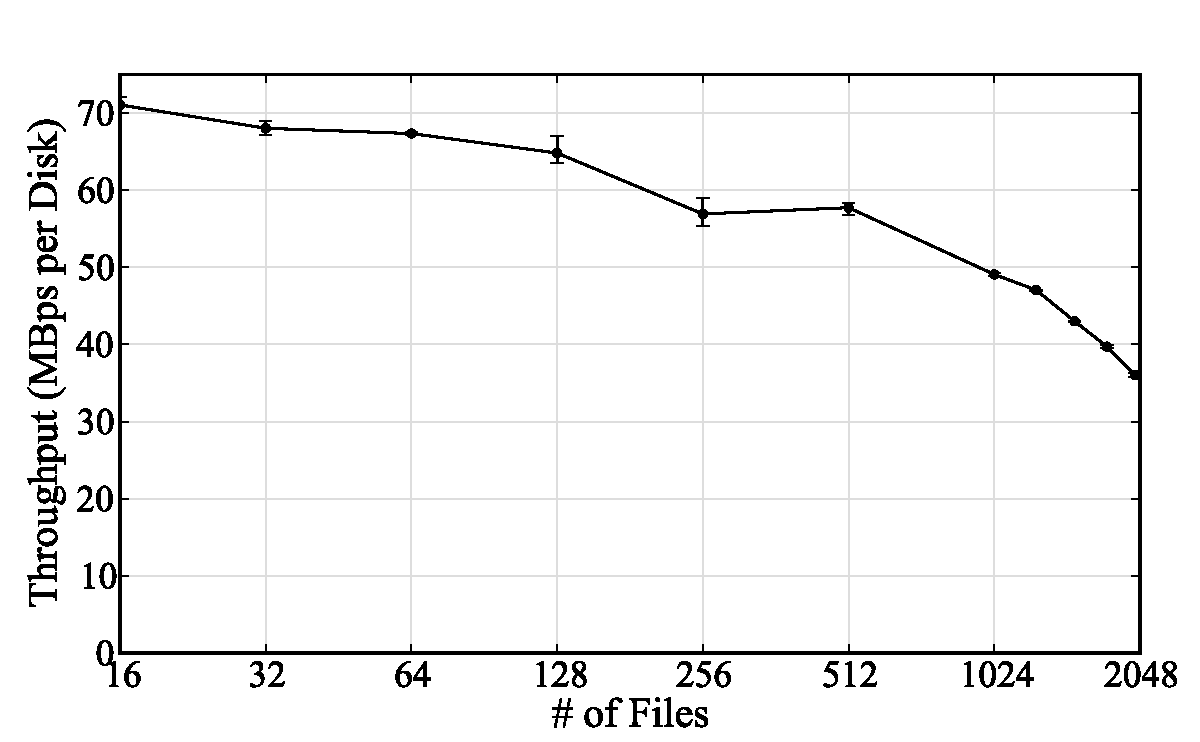
\includegraphics[width=\columnwidth]{tritonsort/graphs/mergesortbench.pdf}
 \caption{\label{fig:mergesort}Performance of the Heaper-Merger sort
   implementation in microbenchmark on a 200GB per disk parallel external merge-sort as a function of the number of files merged per disk.}
\end{figure}

The problem with the Heaper-Merger architecture is that it does not scale well.
In order to prevent the Heaper in phase one from becoming a bottleneck, the the
sorted runs that the Heaper generates are usually fairly small, on the order of
a few hundred megabytes. As a consequence, the number of intermediate files
that the Merger must merge in phase two grows quickly as the size of the input
data increases. This reduces the amount of data from each intermediate file
that can be buffered at a time by the Merger and requires that the merger fetch
additional data from files much more frequently, causing many additional seeks.

To demonstrate this problem, we implemented a simple Heaper-Merger sort module
in microbenchmark. We chose to sort 200GB per disk in parallel across all the
disks to simulate the system's performance during a 100TB sort. Each disk's
200GB data set is partitioned among an increasingly large number of files. Each
node's memory is divided such that each input file and each output file can be
double-buffered. As shown in Figure~\ref{fig:mergesort}, increasing the number
of files being merged causes throughput to decrease dramatically as the number
of files increases above 1000.

\tritonsort uses an alternative architecture with similar software elements as
above and again involving two phases, as mentioned in
Chapter~\ref{chapter:background}.  We partition the input data into a set of
logical \emph{partitions}; with $D$ physical disks and $L$ logical partitions,
each logical partition corresponds to a contiguous $\frac{1}{L}^{th}$ fraction
of the key space and each physical disk hosts $\frac{L}{D}$ logical partitions.
In the first phase, Readers pass buffers directly to Distributors.  A
Distributor maps the key of every record in its input buffer to its
corresponding logical partition and sends that record over the network to the
machine that hosts this logical partition.  Records for a given logical
partition are buffered in memory and written to disk in large chunks in order
to seek as little as possible.  In the second phase, each logical partition is
read into an in-memory buffer, that buffer is sorted, and the sorted buffer is
written to disk.  This scheme bypasses the seek limits of the earlier
mergesort-based approach.  Also, by appropriately choosing the value of $L$, we
can ensure that logical partitions can be read, sorted and written in parallel
in the second phase.  Since our testbed nodes have 24GB of RAM, to ensure this
condition we set the number of logical partitions per node to 2520 so that each
logical partition contains less than 1GB of records when we sort 100 TB on 52
nodes.  We explain this architecture in more detail in the context of our
implementation in the next section.

% LocalWords:  mergesortbench pdf SSD GraySort Infiniband CPUs SATA Heapers th
% LocalWords:  Distributers LocalWords

\section{Design and Implementation}
\label{sec:arch}

\tritonsort is a distributed, staged, pipeline-oriented dataflow processing
system. In this section, we describe \tritonsort's design and motivate our
design decisions for each stage in its processing pipeline.

\subsection{Architecture Overview}

Figures \ref{fig:phase1} and \ref{fig:phase2} show the stages of a \tritonsort
program.  See Chapter~\ref{chapter:principles} for details on how \tritonsort's
stages operate.

In the process of executing its \textit{run()} method, a worker can get buffers
from and return buffers to a shared pool of buffers.  This buffer pool can be
shared among the workers of a single stage, but is typically shared between
workers in pairs of stages with the upstream stage getting buffers from the
pool and the downstream stage putting them back.  When getting a buffer from a
pool, a stage can specify whether or not it wants to block waiting for a buffer
to become available if the pool is empty.

\subsection{Sort Architecture}

We implement sort in two phases.  First, we perform distribution sort to
partition the input data across $L$ logical partitions evenly distributed
across all nodes in the cluster.  Each logical partition is stored in
its own \emph{logical disk}.  All logical disks are of identical maximum size
$size_{LD}$ and consist of files on the local file system.

The value of $size_{LD}$ is chosen such that logical disks
from each physical disk can be read, sorted and written in parallel in the
second phase, ensuring maximum resource utilization.  Therefore, if the size of
the input data is $size_{input}$, there are $L =
\frac{size_{input}}{size_{LD}}$ logical disks in the system.  In phase two, the
records in each logical disk get sorted locally and written to an output file.
This implementation satisfies our design goal of reading and writing each record
twice.

To determine which logical disk holds which records, we logically partition the
10-byte key space into $L$ even divisions.  We logically order the logical
disks such that the $k^{th}$ logical disk holds records in the $k^{th}$
division.  Sorting each logical disk produces a collection of output files,
each of which contains sorted records in a given partition.  Hence, the ordered
collection of output files represents the sorted version of the data.  In this
paper, we assume that records' keys are distributed uniformly over the key
range which ensures that each logical disk is approximately the same size; we
discuss how to handle non-uniform key ranges in Chapter~\ref{chapter:themis}.

To ensure that we can utilize as much read/write bandwidth as possible on each
disk, we partition the disks on each node into two groups of 8 disks each. One
group of disks holds input and output files; we refer to these disks as the
input disks in phase one and as the output disks in phase two.  The other group
holds intermediate files; we refer to these disks as the intermediate disks.
In phase one, input files are read from the input disks and intermediate files
are written to the intermediate disks. In phase two, intermediate files are
read from the intermediate disks and output files are written to the output
disks. Thus, the same disk is never concurrently read from and written to,
which prevents unnecessary seeking.

\subsection{\tritonsort Architecture: Phase One}

\begin{figure*}
  \centering 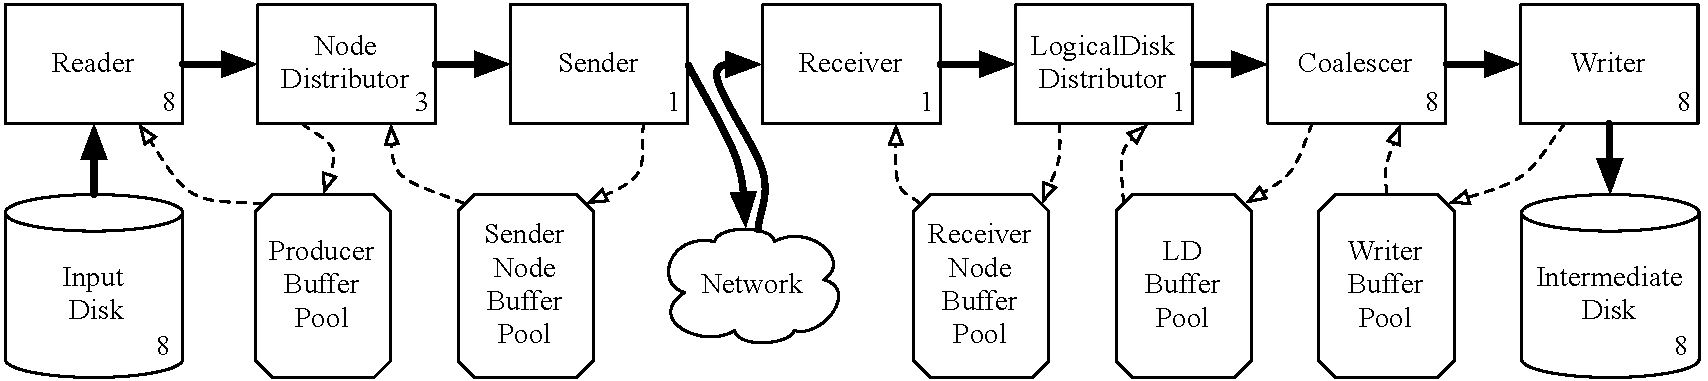
\includegraphics[width=\textwidth]{tritonsort/figs/phase1.pdf}

  \caption{Block diagram of \tritonsort's phase one architecture.  The
    number of workers for a stage is indicated in the lower-right corner of
    that stage's block, and the number of disks of each type is indicated in
    the lower-right corner of that disk's block.}

  \label{fig:phase1}
\end{figure*}

Phase one of \tritonsort, diagrammed in Figure~\ref{fig:phase1}, is responsible
for reading input records off of the input disks, distributing those records
over to the network to the nodes on which they belong, and storing them into
the logical disks in which they belong.

\paragraph{\reader:} Each \reader is assigned an input disk and
is responsible for reading input data off of that disk.  It does this by
filling 80 MB \producerbuffers with input data.
We chose this size because it is large
enough to obtain near sequential throughput from the disk.

\begin{figure}
  \centering
  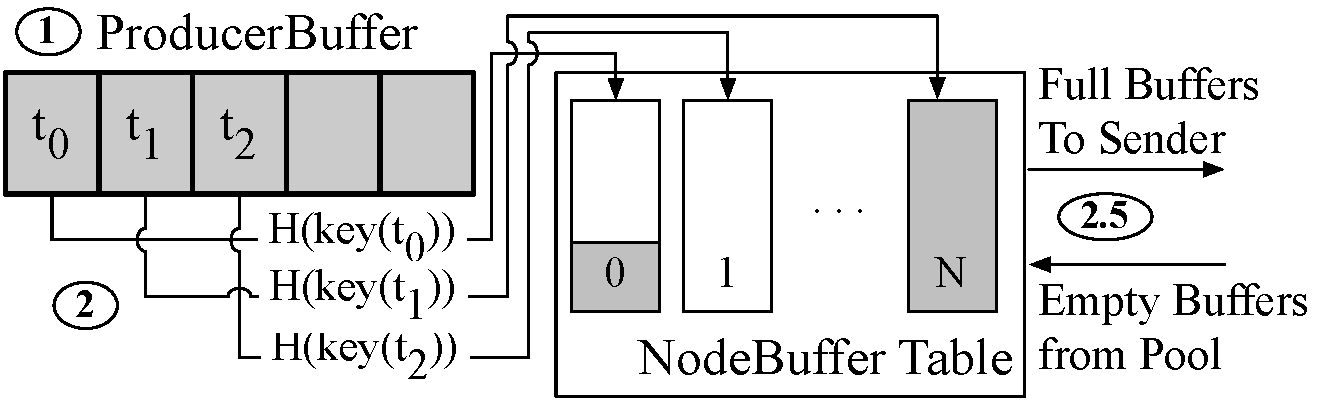
\includegraphics[width=\columnwidth]{tritonsort/figs/pnts_stage.pdf}
  \caption{The \pnts stage, responsible for partitioning records by
    destination node.}
  \label{fig:pnts}
\end{figure}

\paragraph{\pnts:} A \pnts (shown in Figure~\ref{fig:pnts}) receives a
\producerbuffer from a \reader and is responsible for partitioning the records
in that buffer across the machines in the cluster.  It maintains an internal
data structure called a \emph{\nodebuffer table}, which is an array of
\nodebuffers, one for each of the nodes in the cluster.  A \nodebuffer contains
records belonging to the same destination machine.  Its size was chosen to be
the size of the \producerbuffer divided by the number of nodes, and is
approximately 1.6 MB in size for the scales we consider in this paper.

The \pnts scans the \producerbuffer record by record.  For each record, it
computes a hash function $H(k)$ over the record's key $k$ that maps the record to
a unique host in the range $[0,N-1]$.  It uses the \nodebuffer table to select
a \nodebuffer corresponding to host $H(k)$ and appends the record to the end of
that buffer.  If that append operation causes the buffer to become full, the
\pnts removes the \nodebuffer from the \nodebuffer table and sends it
downstream to the \sender stage.  It then gets a new \nodebuffer from the
\nodebuffer pool and inserts that buffer into the newly empty slot in the
\nodebuffer table.  Once the \pnts is finished processing a
\producerbuffer, it returns that buffer back to the \producerbuffer pool.

\begin{figure}
  \centering
  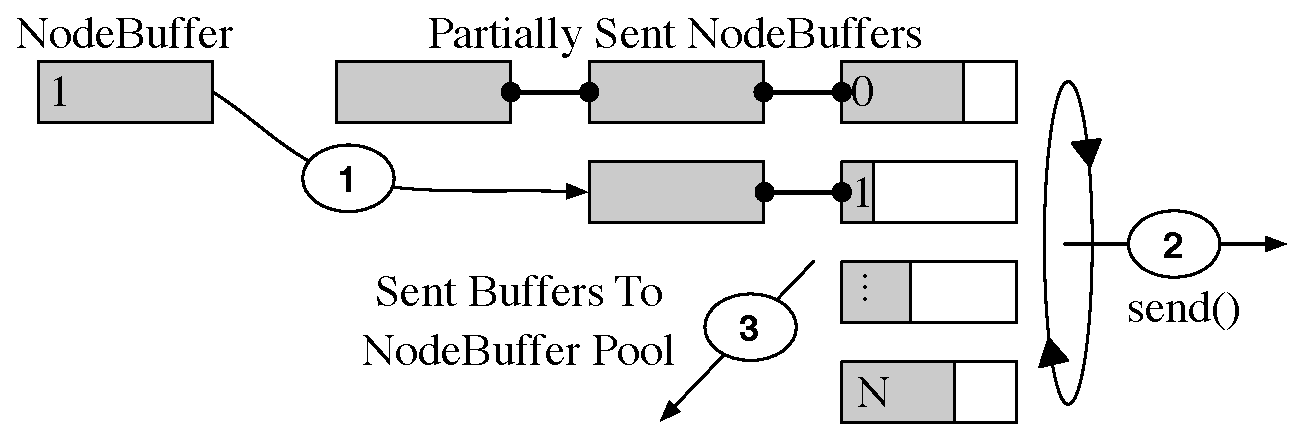
\includegraphics[width=\columnwidth]{tritonsort/figs/sender_stage.pdf}
  \caption{The \sender stage, responsible for sending data to
    other nodes.}
  \label{fig:sender}
\end{figure}

\paragraph{\sender:}  The \sender stage (shown in Figure~\ref{fig:sender}) is
responsible for taking \nodebuffers from the upstream \pnts stage and
transmitting them over the network to each of the other nodes in the cluster.
Each \sender maintains a separate TCP socket per peer node in the cluster.  The
\sender stage can be implemented in a multi-threaded or a single-threaded
manner.  In the multi-threaded case, $N$ \sender workers are instantiated in
their own threads, one for each destination node.  Each \sender worker simply
issues a blocking \textit{send()} call on each \nodebuffer it receives from the
upstream \pnts stage, sending records in the buffer to the appropriate
destination node over the socket open to that node.  When all the records in a
buffer have been sent, the \nodebuffer is returned to its pool, and the next
one is processed.  For reasons described in Section~\ref{sec:fastnetwork}, we
choose a single-threaded \sender implementation instead.  Here, the \sender
interleaves the sending of data across all the destination nodes in small
non-blocking chunks, so as to avoid the overhead of having to activate and
deactivate individual threads for each send operation to each peer.

Unlike most other stages, which process a single unit of work during each
invocation of their \textit{run()} method, the \sender continuously processes
\nodebuffers as it runs, receiving new work as it becomes available from the
\pnts stage.  This is because the \sender must remain active to alternate
between two tasks: accepting incoming \nodebuffers from upstream \pntss, and
sending data from accepted \nodebuffers downstream.  To facilitate accepting
incoming \nodebuffers, each \sender maintains a set of \nodebuffer lists, one
for each destination host.  Initially these lists are empty.  The \sender
appends each \nodebuffer it receives onto the list of \nodebuffers
corresponding to the incoming \nodebuffer's destination node.

To send data across the network, the \sender loops through the elements in the
set of \nodebuffer lists.  If the list is non-empty, the \sender accesses the
\nodebuffer at the head of the list, and sends a fixed-sized amount of data to
the appropriate destination host using a non-blocking \textit{send()} call.  If
the call succeeds and some amount of data was sent, then the \nodebuffer at the
head of the list is updated to note the amount of its contents that have been
successfully sent so far.  If the \textit{send()} call fails, because the TCP
send buffer for that socket is full, that buffer is simply skipped and the
\sender moves on to the next destination host.  When all of the data from a
particular \nodebuffer is successfully sent, the \sender returns that buffer
back to its pool.

\begin{figure}
  \centering 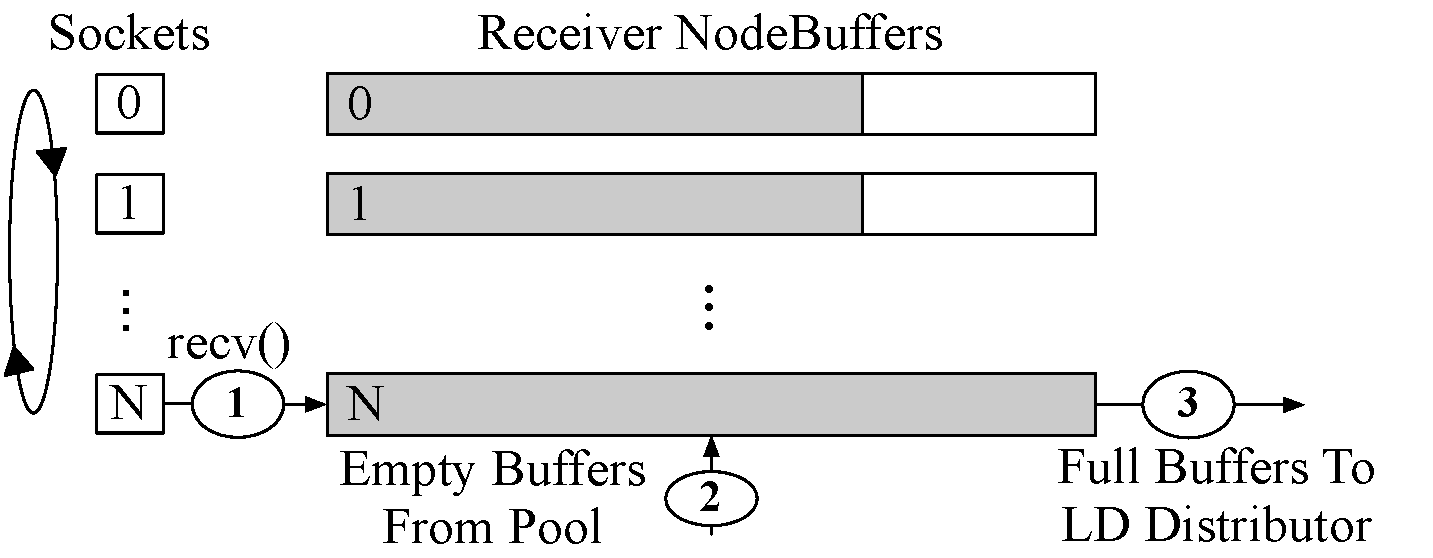
\includegraphics[width=\columnwidth]{tritonsort/figs/receiver_stage.pdf}
  \caption{The \receiver stage, responsible for receiving data from other
    nodes' \sender stages.}
  \label{fig:receiver}
\end{figure}

\paragraph{\receiver:}  The \receiver stage, shown in
Figure~\ref{fig:receiver}, is responsible for receiving data from other nodes
in the cluster, appending that data onto a set of \nodebuffers, and passing
those \nodebuffers downstream to the \ldts stage.  In \tritonsort, the
\receiver stage is instantiated with a single worker.  On starting up, the
\receiver opens a server socket and accepts incoming connections from \sender
workers on remote nodes.  Its \textit{run()} method begins by getting a set of
\nodebuffers from a pool of such buffers, one for each source node.  The
\receiver then loops through each of the open sockets, reading up to 16KB of
data at a time into the \nodebuffer for that source node using a non-blocking
\textit{recv()} call.  This small socket read size is due to the rate-limiting
fix that we explain in Section~\ref{sec:fastnetwork}.  If data is returned by
that call, it is appended to the end of the \nodebuffer.  If the append would
exceed the size of the \nodebuffer, that buffer is sent downstream to the \ldts
stage, and a new \nodebuffer is retrieved from the pool to replace the
\nodebuffer that was sent.

\begin{figure}
  \centering
  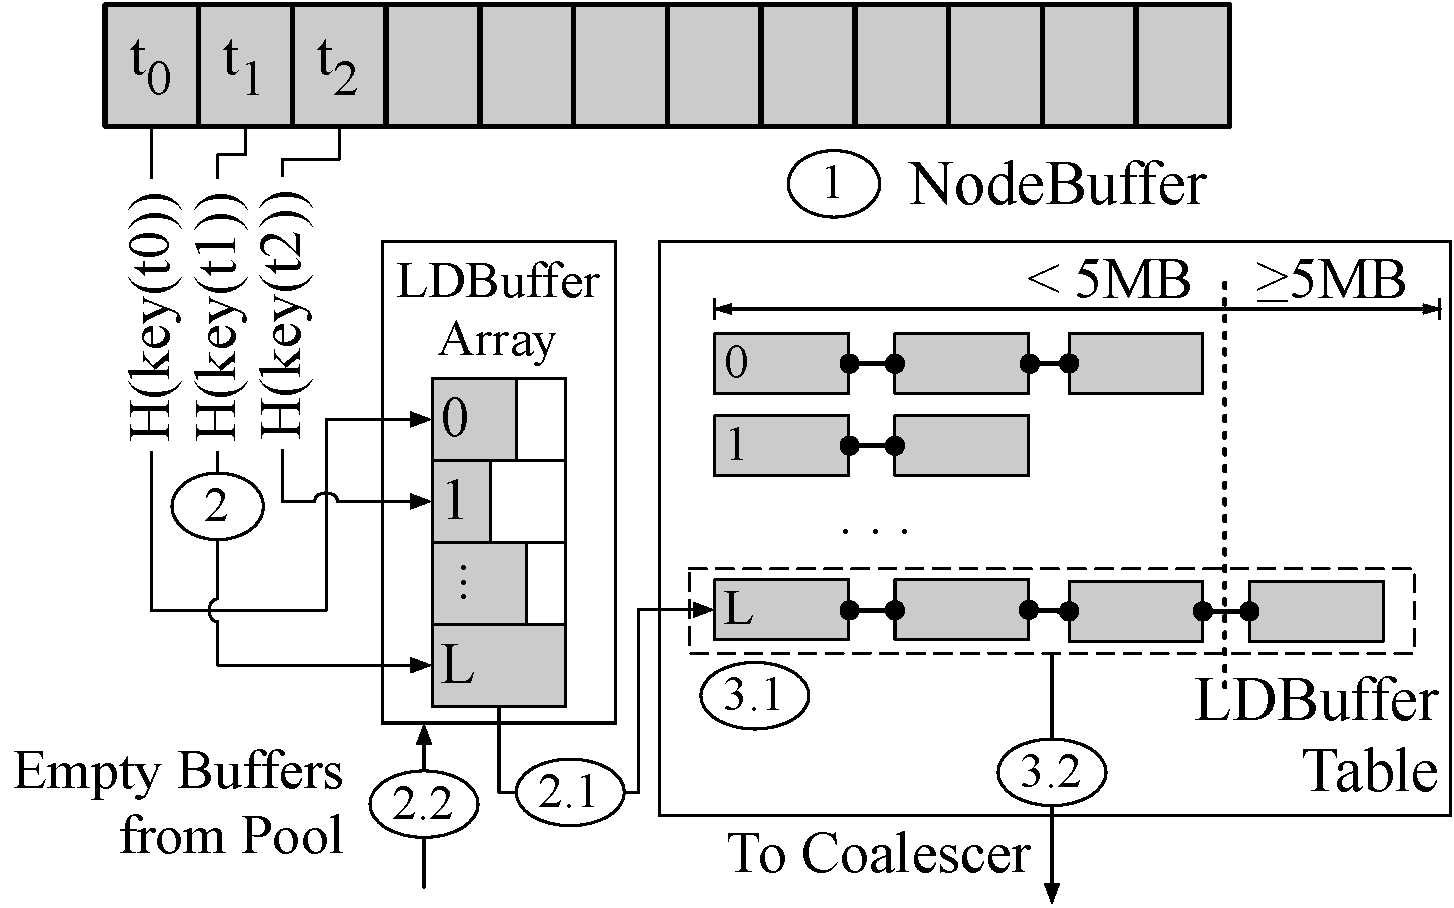
\includegraphics[width=\columnwidth]{tritonsort/figs/ldts_stage.pdf}
  \caption{The \ldts stage, which is responsible for distributing records
  across logical disks and buffering sufficient data to allow for large writes.}
  \label{fig:ldts}
\end{figure}

\paragraph{\ldts:} The \ldts stage, shown in Figure~\ref{fig:ldts}, receives
\nodebuffers from the \receiver that contain records destined for logical disks
on its node.  \ldtss are responsible for distributing records to appropriate
logical disks and sending groups of records destined for the same logical disk to
the downstream \writer stage.

The \ldts's design is driven by the need to buffer enough data to issue large
writes and thereby minimize disk seeks and achieve high bandwidth. Internal to
the \ldts are two data structures: an array of \ldbuffers, one per logical
disk, and an \ldtable.  An \ldbuffer is a buffer of records destined to the same
logical disk.  Each \ldbuffer is 12,800 bytes long, which is the least common
multiple of the record size (100 bytes) and the direct I/O write size (512
bytes).  The \ldtable is an array of \ldbuffer lists, one list per logical disk.
Additionally, \ldts maintains a pool of \ldbuffers, containing 1.25 million
\ldbuffers, accounting for 20 of each machine's 24 GB of memory.

\begin{algorithm}
\begin{algorithmic}[1]
\STATE \nodebuffer $\leftarrow$ getNewWork()\label{alg:ldts:get_work}
\STATE \COMMENT{Drain \nodebuffer into the LDBufferArray}
\FORALL{records $r$ in \nodebuffer}\label{alg:ldts:record_loop_begin}
    \STATE dst $=$ H(key(r))
    \STATE LDBufferArray[dst].append(r)
    \IF{LDBufferArray[dst].isFull()}
        \STATE LDTable.insert(LDBufferArray[dst])
        \STATE LDBufferArray[dst] = getEmptyLDBuffer()
    \ENDIF
\ENDFOR\label{alg:ldts:record_loop_end}

\STATE \COMMENT{Send full LDBufferLists to the Coalescer}
\FORALL{physical disks $d$}\label{alg:ldts:examine_lists_begin}
    \WHILE{LDTable.sizeOfLongestList($d$) $\ge$ 5MB}
        \STATE ld $\leftarrow$ LDTable.getLongestList($d$)
        \STATE \coalescer.pushNewWork(ld)\label{alg:ldts:send_work}
    \ENDWHILE
\ENDFOR\label{alg:ldts:examine_lists_end}
\end{algorithmic}
\caption{The \ldts stage}
\label{alg:ldts}
\end{algorithm}

The operation of a \ldts worker is described in Algorithm~\ref{alg:ldts}. In
Line \ref{alg:ldts:get_work}, a full \nodebuffer is pushed to the \ldts by the
\receiver. Lines \ref{alg:ldts:record_loop_begin}-\ref{alg:ldts:record_loop_end}
are responsible for draining that \nodebuffer record by record into an array of
\ldbuffers, indexed by the logical disk to which the record belongs. Lines
\ref{alg:ldts:examine_lists_begin}-\ref{alg:ldts:examine_lists_end} examine the
\ldtable, looking for logical disk lists that have accumulated enough data to
write out to disk.  We buffer at least 5 MB of data for each logical disk
before flushing that data to disk to prevent many small write requests from
being issued if the pipeline temporarily stalls.  When the minimum threshold of
5 MB is met for any particular physical disk, the longest \ldbuffer list for
that disk is passed to the \coalescer stage on
Line~\ref{alg:ldts:send_work}.

The original design of the \ldts only used the \ldbuffer array described above
and used much larger \ldbuffers (\tilde 10MB each) rather than many small
\ldbuffers. The \coalescer stage (described below) did not exist; instead, the
\ldts transferred the larger \ldbuffers directly to the \writer stage.

This design was abandoned due to its inefficient use of memory. Temporary
imbalances in input distribution could cause \ldbuffers for different logical
disks to fill at different rates.  This, in turn, could cause an \ldbuffer to
become full when many other \ldbuffers in the array are only partially full.
If an \ldbuffer is not available to replace the full buffer, the system must
block (either immediately or when an input record is destined for that buffer's
logical disk) until an \ldbuffer becomes available.  One obvious solution to
this problem is to allow partially full \ldbuffers to be sent to the \writers
at the cost of lower \writer throughput. This scheme introduced the further
problem that the unused portions of the \ldbuffers waiting to be written could
not be used by the \ldts.  In an effort to reduce the amount of memory wasted
in this way, we migrated to the current architecture, which allows small
\ldbuffers to be dynamically reallocated to different logical disks as the need
arises.  This comes at the cost of additional computational overhead and memory
copies, but we deem this cost to be acceptable due to the small cost of memory
copies relative to disk seeks.

\paragraph{\coalescer:} The operation of the \coalescer stage is simple.  A
\coalescer will copy records from each \ldbuffer in its input \ldbuffer list
into a \writerbuffer and pass that \writerbuffer to the \writer stage. It then
returns the \ldbuffers in the list to the \ldbuffer pool.

Originally, the \ldts stage did the work of the \coalescer stage.  While
optimizing the system, however, we realized that the non-trivial amount of time
spent merging \ldbuffers into a single \writerbuffer could be better spent
processing additional \nodebuffers.

\paragraph{\writer:}  The operation of the \writer stage is also quite simple.
When a \coalescer pushes a \writerbuffer to it, the \writer worker will
determine the logical disk corresponding to that \writerbuffer and write out
the data using a blocking \textit{write()} system call.  When the write
completes, the \writerbuffer is returned to the pool.

%\textbf{Possible repeated text.}To ensure maximum utilization of the read/write
%throughput of each disk, we partition the disks on each node into a set of
%input disks and a set of intermediate disks. Further, to reduce contention for
%access to the disks, we assign one \reader worker to every input disk and one
%\writer worker to every intermediate disk. As we show later in our evaluation,
%this setup enables us to balance the operation of the whole system---8 \reader
%workers continuously reading from 8 disks, 8 \writer workers continuously
%writing to 8 other disks, the 10 Gbps network sustaining the data transmitted
%between \sender and \receiver workers, and an appropriate number of \pnts and
%\ldts workers to keep up with the remaining stages.

\subsection{\tritonsort Architecture: Phase Two}

\begin{figure}
  \centering
  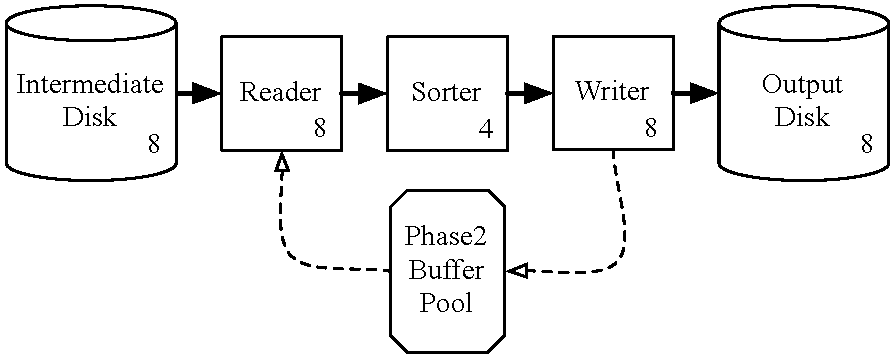
\includegraphics[width=\columnwidth]{tritonsort/figs/phase2.pdf}

  \caption{Block diagram of \tritonsort's phase two architecture.  The
    number of workers for a stage is indicated in the lower-right corner of
    that stage's block, and the number of disks of each type is indicated in
    the lower-right corner of that disk's block.}
  \label{fig:phase2}
\end{figure}

Once phase one completes, all of the records from the input dataset are stored
in appropriate logical disks across the cluster's intermediate disks.  In phase
two, each of these unsorted logical disks is read into memory, sorted, and
written out to an output disk.  The pipeline is straightforward: \reader and
\writer workers issue sequential, streaming I/O requests to the appropriate
disk, and \sorter workers operate entirely in memory.

\paragraph{\reader:}  The phase two \reader stage is identical to
the phase one \reader stage, except that it reads into a \phasetwobuffer, which
is the size of a logical disk.

\paragraph{\sorter:}  The \sorter stage performs an in-memory sort on a
\phasetwobuffer.  A variety of sort algorithms can be used to implement this
stage, however we selected the use of radix sort due to its speed.  Radix sort
requires additional memory overhead compared to an in-place sort like
QuickSort, and so the sizes of our logical disks have to be sized appropriately
so that enough \reader--\sorter--\writer pipelines can operate in parallel.
Our version of radix sort first scans the buffer, constructing a set of
structures containing a pointer to each record's key and a pointer to the record
itself.  These structures are then sorted by key.  Once the structures have
been sorted, they are used to rearrange the records in the buffer in-place. This
reduces the memory overhead for each \sorter substantially at the cost of
additional memory copies.

\paragraph{\writer:}  The phase two \writer writes a \phasetwobuffer
sequentially to a file on an output disk. As in phase one, each \writer is
responsible for writes to a single output disk.

Because the phase two pipeline operates at the granularity of a logical disk,
we can operate several of these pipelines in parallel, limited by either the
number of cores in each system (we can't have more pipelines than cores without
sacrificing performance because the \sorter is CPU-bound), the amount of
memory in the system (each pipeline requires at least three times the size of a
logical disk to be able to read, sort, and write in parallel), or the
throughput of the disks.  In our case, the limiting factor is the
output disk bandwidth.  To host one phase two pipeline per input
disk requires storing 24 logical disks in memory at a time.  To
accomplish this, we set $size_{LD}$ to 850 MB, using most of the 24 GB of RAM
available on each node and allowing for additional memory required by the
operating system.  To sort 850 MB logical disks fast enough to not block the
\reader and \writer stages, we find that four \sorters suffice.

\subsection{Stage and Buffer Sizing}

One of the major requirements for operating \tritonsort at near disk speed is
ensuring cross-stage balance.  Each stage has an intrinsic execution time,
either based on the speed of the device to which it interfaces (e.g., disks or
network links), or based on the amount of CPU time it requires to process a
work unit.  Table~\ref{tbl:stageruntimes} shows the speed and performance of
each stage in the pipeline.  In our implementation, we are limited by the speed
of the \writer stage in both phases one and two.

\begin{table*}
\caption{\label{tbl:stageruntimes}Median stage runtimes for a 52-node,
  100TB sort, excluding the amount of time spent waiting for buffers.}
\centering
\resizebox{\columnwidth}{!}{%
\begin{tabular}{|c|c|c|c|c|c|}
\hline
\textbf{Worker Type} & \textbf{Size Of} & \textbf{Runtime} & \textbf{\# Workers} & \textbf{Throughput} & \textbf{Total Throughput} \\
& \textbf{Input (MB)} & \textbf{(ms)} & & \textbf{(in MBps)} & \textbf{(in MBps)} \\
\hline
\reader    & 81.92 & 958.48 & 8 & 85    & 683 \\
\pnts      & 81.92 & 263.54 & 3 & 310   & 932 \\
%\sender    & 1.65  & 1.38  & 1 & 1188  & 1188 \\
%\receiver  & 1.65  & 1.38  & 1 & 1188  & 1188 \\
\ldts      & 1.65  & 2.42   & 1 & 683   & 683 \\
\coalescer & 10.60  & 4.56   & 8 & 2,324 & 18,593 \\
\writer    & 10.60  & 141.07 & 8 & 75    & 601 \\
\hline
Phase two \reader & 762.95 & 8,238 & 8 & 92 & 740 \\
Phase two \sorter & 762.95 & 2,802 & 4 & 272 & 1089 \\
Phase two \writer & 762.95 & 8,512 & 8 & 89 & 717 \\
\hline
\end{tabular}%
}
\end{table*}

% LocalWords:  enqueueing enqueued dataflow priori getNewWork isFull Coalescer
% LocalWords:  getEmptyLDBuffer LDBufferLists sizeOfLongestList pushNewWork
% LocalWords:  getLongestList dataset QuickSort Runtime runtimes LocalWords

\section{Optimizations}
\label{sec:optimizations}

In implementing \tritonsort, we learned that several non-obvious optimizations
were necessary to meet our desired disk bandwidth goals.  Here, we present the
key takeaways from our experience.

\subsection{Network}
\label{sec:fastnetwork}

\begin{figure}
  \centering
  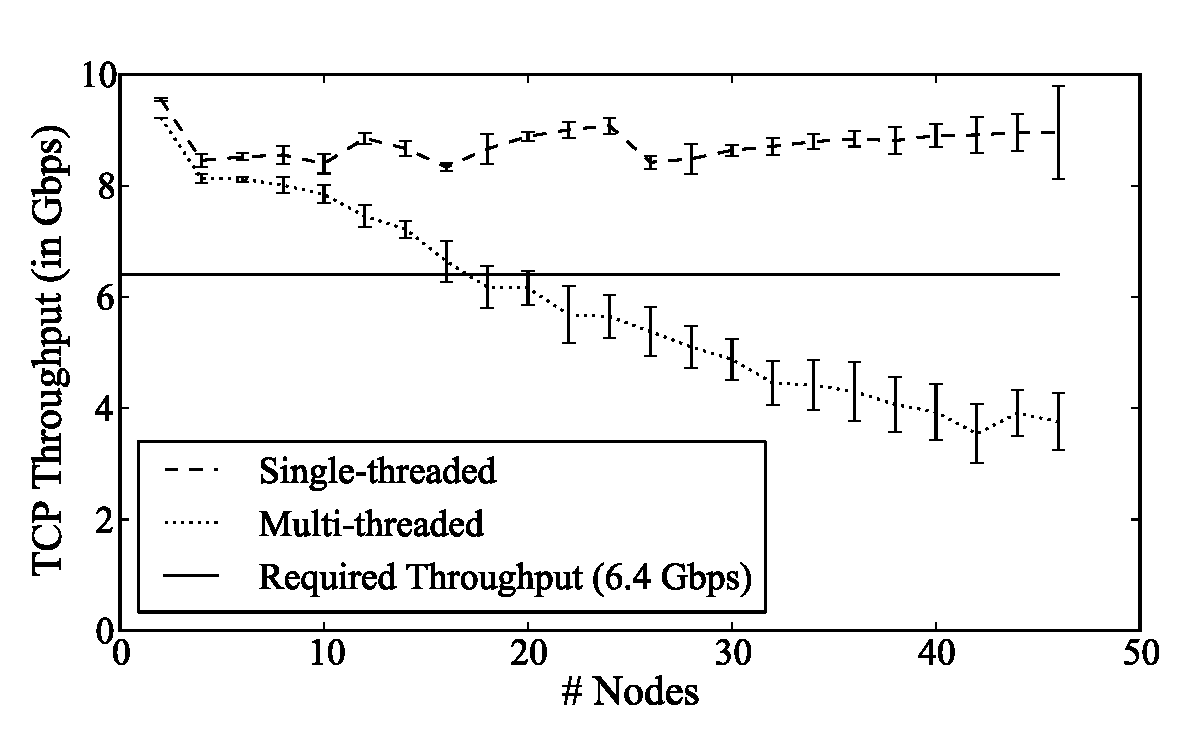
\includegraphics[width=\columnwidth]{tritonsort/graphs/netscalability.pdf}

\caption{Comparing the scalability of single-threaded and
  multi-threaded \receiver implementations}
  \label{fig:net_scalability}
\end{figure}

For \tritonsort to operate at the aggregate sequential streaming bandwidth of
all of its disks, the network must be able to sustain the read throughput of
eight disks while data is being shuffled among nodes in the first phase.  Since
the 7.2k-RPM disks we use deliver at most 100 MBps of sequential read
throughput (Table~\ref{tab:resourcesummary}), the network must be able to
sustain 6.4 Gbps of all-pairs bandwidth, irrespective of the number of nodes in
the cluster.

It is well-known that sustaining high-bandwidth flows in datacenter networks,
especially all-to-all patterns, is a significant challenge.  Reasons for this
include commodity datacenter network hardware, incast, queue buildup, and
buffer pressure\cite{dctcp}.  Since we could not employ a strategy like that
presented in \cite{dctcp} to provide fair but high bandwidth flow rates among
the senders, we chose instead to artificially rate limit each flow at the
\sender stage to its calculated fair share by forcing the sockets to be receive
window limited.  This works for \tritonsort because 1) each machine sends and
receives at approximately the same rate, 2) all the nodes share the same RTT
since they are interconnected by a single switch, and 3) our switch
does not impose an oversubscription factor.  In this case, each \sender should
ideally send at a rate of $(6.4 / N)$ Gbps, or 123 Mbps with a cluster of 52
nodes.  Given that our network offers approximately $100 \mu{}sec$ RTTs, a
receiver window size of $8-16$ KB ensures that the flows will not impose queue
buildup or buffer pressure on other flows.

Initially, we chose a straightforward multi-threaded design for the \sender and
\receiver stages in which there were $N$ \senders and $N$ \receivers, one for
each \tritonsort node.  In this design, each \sender issues blocking
\textit{send()} calls on a \nodebuffer until it is sent.  Likewise, on the
destination node, each \receiver repeatedly issues blocking \textit{recv()}
calls until a \nodebuffer has been received.  Because the number of CPU
hyperthreads on each of our nodes is typically much smaller than $2N$, we
pinned all \senders' threads to a single hyperthread and all \receivers'
threads to a single separate hyperthread.

Figure~\ref{fig:net_scalability} shows that this multi-threaded approach does
not scale well with the number of nodes, dropping below 4 Gbps at scale.  This
poor performance is due to thread scheduling overheads at the end hosts.  16 KB
TCP receive buffers fill up much faster than connections that are not
window-limited.  At the rate of 123 MBps, a 16 KB buffer will fill up in just
over 1 ms, causing the \sender to stop sending.  Thus, the \receiver stage must
clear out each of its buffers at that rate.  Since there are 52 such buffers, a
\receiver must visit and clear a receive buffer in just over 20 $\mu$s.  A
\receiver worker thread cannot drain the socket, block, go to sleep, and get
woken up again fast enough to service buffers at this rate.

To circumvent this problem we implemented a single-threaded, non-blocking
receiver that scans through each socket in round-robin order, copying out any
available data and storing it in a \nodebuffer during each pass through the
array of open sockets.  This implementation is able to clear each socket's
receiver buffer faster than the arrival rate of incoming data.
Figure~\ref{fig:net_scalability} shows that this design scales well as the
cluster grows.

\subsection{Minimizing Disk Seeks}
\label{sec:diskseeks}

\begin{figure}
  \centering
  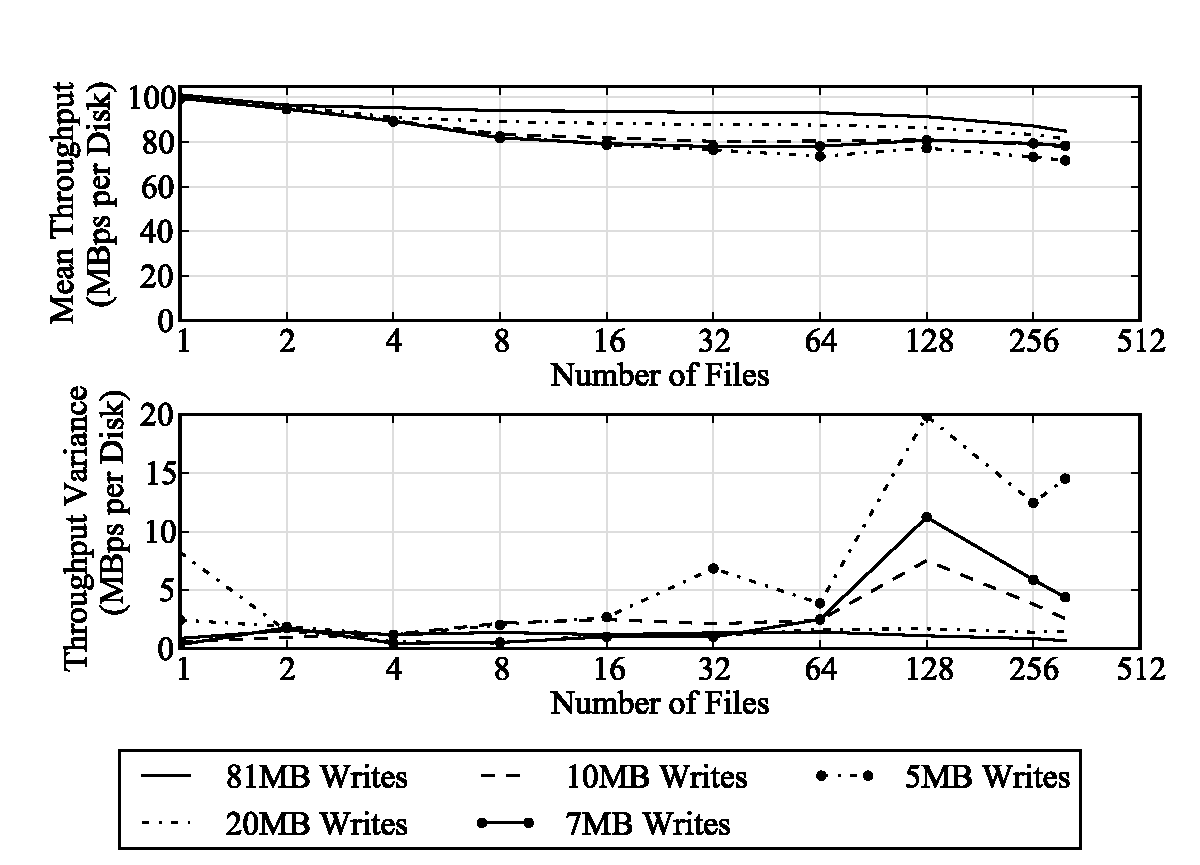
\includegraphics[width=\columnwidth]{tritonsort/graphs/write_scalability_throughput_receiverbench}
  \caption{\label{fig:micro_write_bw}Microbenchmark indicating the ideal disk throughput as a function of
           write size}
\end{figure}

Key to making the \tritonsort pipeline efficient is minimizing the total amount
of time spent performing disk seeks, both while writing data in phase one, and
while reading that data in phase two.  As individual write sizes get smaller,
write throughput drops, since the disk must occasionally seek between
individual write operations.  Figure~\ref{fig:micro_write_bw} shows disk write
throughput measured by a synthetic workload generator writing to a configurable
set of files with different write sizes.  Ideally, the \writer would receive
\writerbuffers large enough that it can write them out at close to the
sequential rate of the disk.  However, the amount of available memory limits
\tritonsort's write sizes.  Since the record space is uniformly distributed
across the logical disks, the \ldts will fill its \ldbuffer{}s at approximately
a uniform rate.  Buffering 80 MB worth of records for a given logical disk
before writing to disk would cause the buffers associated with all of the other
logical disks to become approximately as full.  This would mandate
significantly higher memory requirements than what is available in our hardware
architecture.  Hence, the \ldts stage must emit smaller \writerbuffer{}s, and
it must interleave writes to different logical disks.

\subsection{The Importance of File Layout}

The physical layout of individual logical disk files plays a strong role in
trading off performance between the phase one \writer and the phase two
\reader.  One strategy is to append to the logical disk files in a
log-structured manner, in which a \writerbuffer for one logical disk is
immediately appended after the \writerbuffer for a different logical disk.
This is possible if the logical disks' blocks are allocated on demand.  It has
the advantage of making the phase one \writer highly performant, since it
minimizes seeks and leads to near-sequential write performance.  On the other
hand, when a phase two \reader begins reading a particular logical disk, the
underlying physical disk will need to seek frequently to read each of the
\writerbuffer{}s making up the logical disk.

An alternative approach is to greedily allocate all of the blocks for each of
the logical disks at start time, ensuring that all of a logical disk's blocks
are physically contiguous on the underlying disk.  This can be accomplished
with the \texttt{fallocate()} system call, which provides a hint to the file
system to pre-allocate blocks.  In this scheme, interleaved writes of
\writerbuffer{}s for different logical disks will require seeking, since two
subsequent writes to different logical disks will need to write to different
regions on the disk.  However, in phase two, the \reader will be able to
sequentially read an entire logical disk with minimal seeking. We also use
\texttt{fallocate()} on input and output files so that phase one \readers and
phase two \writers seek as little as possible.

The location of output files on the output disks also has a dramatic effect on
phase two's performance.  If we do not delete the input files before starting
phase two, the output files are allocated space on the interior cylinders of
the disk.  When evaluating phase two's performance on a 100 TB sort, we found
that we could write to the interior cylinders of the disk at an average rate of
~64 MBps.  When we deleted the input files before phase two began, ensuring that
the output files would be written to the exterior cylinders of the disk, this
rate jumped to 84 MBps.  For the evaluations in Section~\ref{sec:evaluation}, we
delete the input files before starting phase two.  For reference, the fastest
we have been able to write to the disks in microbenchmark
has been approximately 90 MBps.

\subsection{CPU Scheduling}

Modern operating systems support a wide variety of static and dynamic CPU
scheduling approaches, and there has been considerable research into scheduling
disciplines for data processing systems.  We put a significant amount of effort
into isolating stages from one another by setting the processor affinities of
worker threads explicitly, but we eventually discovered that using the default
Linux scheduler results in a steady-state performance that is only about 5\%
worse than any custom scheduling policy we devised.  In our evaluation, we use
our custom scheduling policy unless otherwise specified.

\subsection{Pipeline Demand Feedback}

Initially, \tritonsort was entirely ``push''-based, meaning that a worker only
processed work when it was pushed to it from a preceding stage.  While simple
to design, certain stages perform sub-optimally when they are unable to send
feedback back in the pipeline as to what work they are capable of doing.  For
example, the throughput of the \writer stage in phase one is limited by the
latency of writes to the intermediate disks, which is governed by the sizes of
\writerbuffer{}s sent to it as well as the physical layout of logical disks
(due to the effects of seek and rotational delay).  In its \naive
implementation, the \ldts sends work to the \writer stage based on which of its
\ldbuffer lists is longest with no regard to how lightly or heavily loaded the
\writers themselves are.  This can result in an imbalance of work across
\writers, with some \writers idle and others struggling to process a long queue
of work.  This imbalance can destabilize the whole pipeline and lower total
throughput.

To address this problem, we must effectively communicate information about the
sizes of \writers' work queues to upstream stages.  We do this by creating a
pool of \emph{write tokens}. Every write token is assigned a single ``parent''
\writer. We assign parent \writers in round-robin order to tokens as the tokens
are created and create a number of tokens equal to the number of
\writerbuffers.
When the \ldts has buffered enough \ldbuffers so that one or more of its logical
disks is above the minimum write threshold (5MB), the \ldts will query the
write token pool, passing it a set of \writers for which it has enough data.
If a write token is available for one of the specified \writers in the set, the
pool will return that token; otherwise, it will signal that no tokens are
available.  The \ldts is required to pass a token for the target \writer along
with its \ldbuffer list to the next stage, This simple mechanism prevents any
\writer's work queue from growing longer than its ``fair share'' of the
available \writerbuffers and provides reverse feedback in the pipeline without
adding any new architectural features.

\subsection{System Call Behavior}

In the construction of any large system, there are always idiosyncrasies in
performance that must be identified and corrected.  For example, we noticed
that the sizes of arguments to Linux \texttt{write()} system calls had a
dramatic impact on their latency; issuing many small writes per buffer often
yielded more performance than issuing a single large write.  One would imagine
that providing more information about the application's intended behavior to
the operating system would result in better management of underlying resources
and latency but in this case, the opposite seems to be true.  While we are
still unsure of the cause of this behavior, it illustrates that the performance
characteristics of operating system services can be unpredictable and
counter-intuitive.

%LocalWords: incast RTT oversubscription Mbps RTTs recv hyperthreads epoll
%LocalWords: Microbenchmark record records performant pre microbenchmark

\section{Evaluation}
\label{sec:evaluation}

We now evaluate \tritonsort's performance and scalability under
various hardware configurations.

\subsection{Evaluation Environment}

We evaluated \tritonsort on 52 nodes of the cluster described in
Section~\ref{sec:hardware_architecture}.  Each XFS partition is configured with
a single allocation group to prevent file fragmentation across allocation
groups, and is mounted with the \texttt{noatime}, \texttt{attr2},
\texttt{nobarrier}, and \texttt{noquota} flags set.  For this evaluation, the
servers were running Linux 2.6.35.1. Our implementation of \tritonsort is
written in C++.

\subsection{Comparison to Alternatives}

The 100TB Indy GraySort benchmark was introduced in 2009, and hence there are
few systems against which we can compare \tritonsort's performance. The most
recent holder of the Indy GraySort benchmark, DEMSort~\cite{DEMSort}, sorted
slightly over 100TB of data on 195 nodes at a rate of 564 GB per minute.
\tritonsort currently sorts 100TB of data on \tsnodes nodes at a rate of
\tsrate GB per minute, a factor of \tsimprovementfactor improvement in per-node
efficiency.

\subsection{Examining Changes in Balance}

We next examine the effect of changing the cluster's configuration to support
more memory or faster disks. Due to budgetary constraints, we could not
evaluate these hardware configurations at scale. Evaluating
the performance benefits of SSDs is the subject of future work.

In the first experiment, we replaced the 500GB, 7200RPM disks that are used as
the intermediate disks in phase one and the input disks in phase two with
146GB, 15000RPM disks. The reduced capacity of the drives necessitated running
an experiment with a smaller input data set.  To allow space for the logical
disks to be pre-allocated on the intermediate disks without overrunning the
disks' capacity, we decreased the number of logical disks per physical disk by
a factor of two. This doubles the amount of data in each logical disk, but the
experiment's input data set is small enough that the amount of data per logical
disk does not overflow the logical disk's maximum size.

Phase one throughput in these experiments is slightly lower than in subsequent
experiments because the 30-35 seconds it takes to write the last few bytes of
each logical disk at the end of the phase is roughly 10\% of the total runtime
due to the relatively small dataset size.

\begin{table*}
\centering
\caption{\label{table:15k}Effect of increasing speed of intermediate disks
  on a two node, 500GB sort.}
\resizebox{\columnwidth}{!}{%
\begin{tabular}{|c|c|c|c|c|}
\hline
\textbf{Intermediate Disk} & \textbf{Logical Disks}  & \textbf{Phase 1} &
\textbf{Phase 1} & \textbf{Average Write} \\
\textbf{Speed (RPM)} & \textbf{Per Physical Disk} & \textbf{Throughput (MBps)} & \textbf{Bottleneck Stage} & \textbf{Size (MB)}\\
\hline
7200 & 315 & 69.81 &  \writer & 12.6  \\
7200 & 158 & 77.89 &  \writer & 14.0  \\
15000 & 158 & 79.73 &  \ldts  & 5.02 \\
\hline
\end{tabular}%
}
\end{table*}

The results of this experiment are shown in Table~\ref{table:15k}.  We first
examine the effect of decreasing the number of logical disks without increasing
disk speed. Decreasing the number of logical disks increases the average length
of \ldbuffer chains formed by the \ldts; note that most of the time, full
\writerbuffers (14MB) are written to the disks. In addition, halving the number
of logical disks decreases the number of external cylinders that the logical
disks occupy, decreasing maximal seek latency. These two factors combine
together to net a significant (11\%) increase in phase one throughput.

The performance gained by writing to 15000 RPM disks in phase one is much less
pronounced. The main reason for this is that the increase in write speed causes
the \writers to become fast enough that the \ldts exposes itself as the
bottleneck stage. One side-effect of this is that the
\ldts cannot populate \writerbuffers as fast as they become available, so it
reverts to a pathological case in which it always is able to successfully
retrieve a write token and hence continuously writes minimally-filled (5MB)
buffers. Creating a \ldts stage that dynamically adjusts its write size based
on write token retrieval success rate is the subject of future work.


\begin{table}
\centering
\caption{\label{table:bigmem}Effect of increasing the amount of memory per
  node on a two node, 2TB sort.}
\begin{tabular}{|c|c|c|}
\hline
\textbf{RAM Per}  & \textbf{Phase 1}  & \textbf{Average Write} \\
\textbf{Node (GB)} & \textbf{Throughput (MBps)} & \textbf{Size (MB)} \\
\hline
24 & 73.53 & 12.43 \\
48 & 76.45 & 19.21 \\
\hline
\end{tabular}
\end{table}

In the next experiment, we doubled the RAM in two of the machines in our
cluster and adjusted \tritonsort's memory allocation by doubling the size of
each \writerbuffer (from 14MB to 28MB) and using the remaining memory (22GB)
to create additional \ldbuffers. As shown in Table~\ref{table:bigmem},
increasing the amount of memory allows for the creation of longer chains of
\ldbuffers in the \ldts, which in turn causes write sizes to increase. The
increase in write size is not linear in the amount of RAM added; this is likely
because we are approaching the point past which larger writes will not
dramatically improve write throughput.

\subsection{\tritonsort Scalability}

\begin{figure}[T]
    \centering
    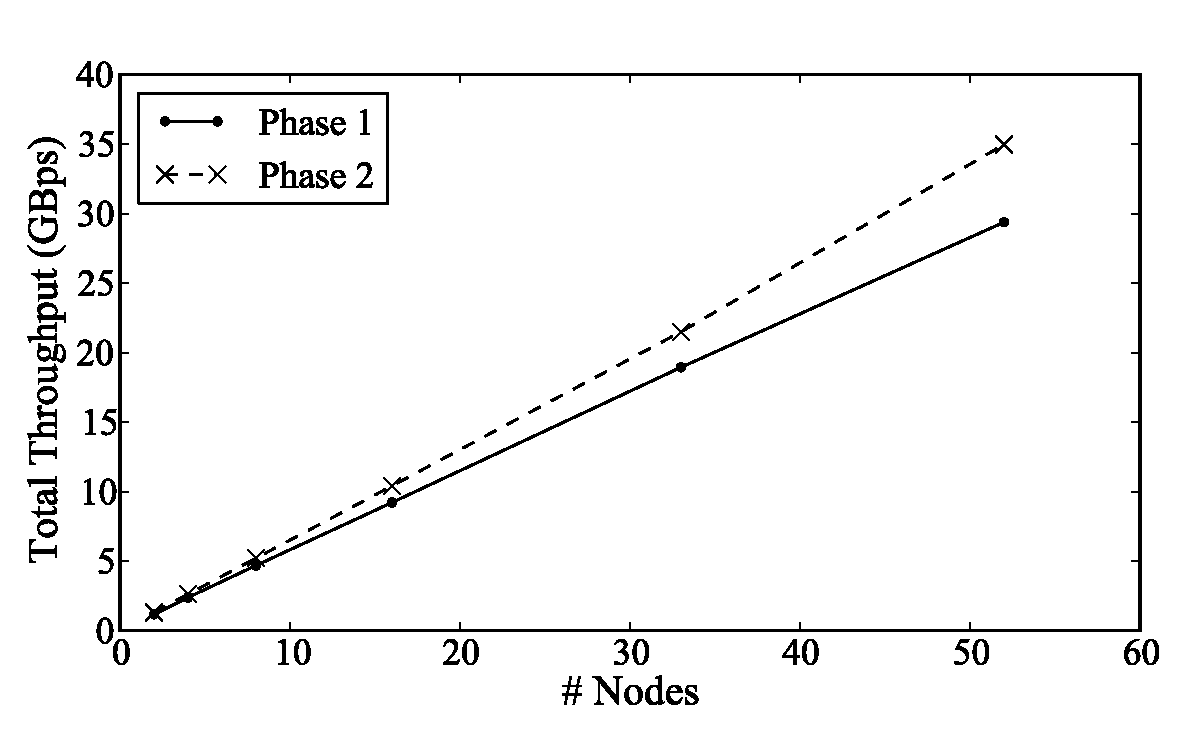
\includegraphics[width=\columnwidth]{tritonsort/graphs/scalability.pdf}

    \caption{\label{fig:scalability}Throughput when sorting 1 TB per node as the number of nodes increases.}
\end{figure}

Figure~\ref{fig:scalability} shows \tritonsort's total throughput when sorting
1 TB per node as the number of nodes increases from 2 to 48. Phase two exhibits
practically linear scaling, which is expected since each node performs phase
two in isolation.  Phase one's scalability is also nearly linear; the slight
degradation in its performance at large scales is likely due to network
variance that becomes more pronounced as the number of nodes increases.

%LocalWords: LocalWords noquota dataset runtime

\section{Conclusions}
\label{tritonsort:sec:conclusions}

In this work, we describe the hardware and software architecture necessary to
build \tritonsort, a highly efficient, pipelined, stage-driven sorting system
designed to sort tens to hundreds of TB of data.  Through careful management of
system resources to ensure cross-resource balance, we are able to sort tens of
GB of data per node per minute, resulting in \tsrate GB/min across only
\tsnodes nodes.  We believe the work holds a number of lessons for balanced
system design and for scale-out architectures in general and will help inform
the construction of more balanced data processing systems that will bridge the
gap between scalability and per-node efficiency.

%LocalWords: LocalWords pipelined


\section{Acknowledgments}

This project was supported by NSF's Center for Integrated Access Networks and
NSF MRI \#CNS-0923523.  We'd like to thank Cisco Systems for their support of
this work.  We'd like to acknowledge Stefan Savage for providing valuable
feedback concerning network optimizations, and thank our shepherd Andrew
Birrell and the anonymous reviewers for their feedback and suggestions.

%LocalWords: Birrell NSF's Cisco LocalWords

Chapter~\ref{chapter:tritonsort} contains material as it appears in the
Proceedings of the USENIX Symposium on Networked Systems Design and
Implementation (NSDI) 2011. Rasmussen, Alexander; Porter, George; Conley,
Michael; Madhyastha, Harsha; Niranjan Mysore, Radhika; Pucher, Alexander;
Vahdat, Amin. The dissertation author was the primary investigator and author
of this paper.


\chapter{Themis: I/O-Efficient MapReduce}
\label{chapter:themis}

This chapter presents Themis\footnote{Themis is a Titan in Greek mythology who
  is tasked with creating balance, order and harmony.}, an I/O-efficient
MapReduce system derived from TritonSort.

Many MapReduce jobs are I/O-bound, and so minimizing the number of I/O
operations is critical to improving their performance. Themis reads and writes
data records to disk exactly twice, which is the minimum amount possible for
data sets that cannot fit in memory.

In order to minimize I/O, Themis makes fundamentally different design decisions
from previous MapReduce implementations. Themis performs a wide variety of
MapReduce jobs -- including click log analysis, DNA read sequence alignment,
and PageRank -- at nearly the speed of TritonSort's record-setting sort
performance.

\section{Introduction}
\label{themis:sec:intro}

Our experience building TritonSort shows that an appropriately balanced
implementation can realize orders of magnitude improvement in throughput and
efficiency.  Translating these types of gains to more general-purpose data
processing systems will help close the efficiency gap present in modern
large-scale data processing systems, allowing more work to be performed with
the same hardware, or the same amount of work to be performed with less
hardware. This improved efficiency will result in substantially lowered system
cost, energy usage, and management complexity.

Given that many MapReduce jobs are I/O-bound, an efficient MapReduce system
must aim to minimize the number of I/O operations it performs.  Fundamentally,
every MapReduce system must perform at least two I/O operations per record when
the amount of data exceeds the amount of memory in the cluster~\cite{sort-io}.
We refer to a system that meets this lower-bound as having the ``2-IO''
property.  Any data processing system that does not have this property is doing
more I/O than it needs to.  Existing MapReduce systems incur additional I/O
operations in exchange for simpler and more fine-grained fault tolerance.

Themis is an implementation of MapReduce designed to have the 2-IO
property. Themis accommodates the flexibility of the MapReduce programming
model while simultaneously delivering high efficiency.  It does this by
considering fundamentally different points in the design space than existing
MapReduce implementations:

\paragraph{1. Eliminating task-level fault tolerance:} At the scale of tens of
thousands of servers, failures are common, and so MapReduce was designed with a
strong task-level fault tolerance model.  However, more aggressive fault
tolerance gains finer-grained restart at the expense of lower overall
performance.  Interestingly, many Hadoop users report cluster sizes of under
100 nodes~\cite{HadoopPoweredBy}, much smaller than those deployed by
MapReduce's early adopters.  In 2011, Cloudera's VP of Technology Solutions
stated that the mean size of their clients' Hadoop clusters is 200 nodes, with
the median size closer to 30~\cite{MonashTrajman}.  At this moderate scale,
failures are much less common, and aggressive fault tolerance is wasteful in
the common case.  Foregoing task-level fault tolerance permits a design that
achieves the 2-IO property.  When a job experiences a failure, Themis simply
re-executes it.  This optimistic approach to fault tolerance enables Themis to
aggressively pipeline record processing without unnecessarily materializing
intermediate results to disk.  As we will show in
Chapter~\ref{chapter:fault_tolerance}, for moderate cluster sizes this approach
has the counter-intuitive effect of improving performance despite the
occasional job re-execution.

\paragraph{2. Dynamic, adaptive memory allocation:} To maintain the 2-IO
property, Themis must process a record completely once it is read from disk.
This prevents Themis from putting records back on disk in response to memory
pressure through swapping or writing spill files.  Themis implements a
policy-based, application-level memory manager that provides fine-grained
sharing of memory between operators processing semi-structured, variably-sized
records.  This allows it to support datasets with as much as a factor of
$10^7$ skew between record sizes while maintaining the 2-IO property.

\paragraph{3. Central management of shuffle and disk I/O:} Themis uses a
centralized, per-node disk scheduler that ensures that records from multiple
sources are written to disk in large batches to reduce disk seeks.  Themis
delivers nearly sequential disk I/O across a variety of MapReduce jobs, even
for workloads that far exceed the size of main memory.

To validate our design, we have written a number of MapReduce programs on
Themis, including a web user session tracking application, PageRank, n-gram
counting, and a DNA read sequence alignment application.  We found that Themis
processes these jobs at nearly the per-node performance of TritonSort's
record-setting sort run and nearly the maximum sequential speed of the
underlying disks.

\section{The Challenge of Skew}
\label{themis:sec:challenges}

One of MapReduce's attractive properties is its ability to handle
semi-structured and variably-sized data.  This variability makes maintaining
the 2-IO property a challenge.  In this section, we describe two sources of
variability and the resulting requirements they place on our design.

An input dataset can exhibit several different kinds of \emph{skew},
which simply refers to variability in its structure and content.  These
include:

\paragraph{Record Size Skew:} In systems with semi-structured or unstructured
data, some records may be much larger than others.  This is called \emph{record
  size skew}.  In extreme cases, a single record may be gigabytes in size.

\paragraph{Partitioning Skew:} Data that is
not uniformly distributed across its keyspace exhibits \emph{partitioning
  skew}.  This can cause some nodes to process much more data than others if
the data is na\"{\i}vely partitioned across nodes, creating
stragglers~\cite{DeWittGraySkew}.  Handling skew in MapReduce is complicated by
the fact that the distribution of keys in the data produced by a \map function
is often not known in advance.  Existing MapReduce implementations handle
partitioning skew by spilling records to disk that cannot fit into memory.

\paragraph{Computational Skew:} In a dataset exhibiting
\emph{computational skew}, some records take much longer than average to
process.  Much of the work on mitigating computational skew in MapReduce
involves exploiting the nature of the particular problem and relying on a
degree of user guidance~\cite{SkewReduce} or proactively re-partitioning
the input data for a task~\cite{SkewTune}.  As the focus of our work is
I/O-bound jobs, we do not consider computational skew in this work.

\paragraph{Performance Heterogeneity:} The performance of a
population of identical machines can vary significantly; the reasons for this
heterogeneity are explored in \cite{stutterfault}. In addition, clusters are
rarely made up of a homogeneous collection of machines, due both to machine
failures and planned incremental upgrades. While we believe that the techniques
presented in this work can be applied to heterogeneous clusters, we have not
evaluated Themis in such a setting.

To handle record skew, Themis dynamically controls its memory usage, which we
describe in Section~\ref{sec:memory}.  Themis adopts a sampling-based skew
mitigation technique to minimize the effects of partitioning skew.  We discuss
this mitigation technique in Section~\ref{sec:phase_zero}.

\section{System Architecture}
\label{sec:design}

In this section, we describe the design of Themis.

\subsection{Core Architecture}
\label{sec:overview}

Themis reuses several core runtime components that were used to build
TritonSort.  Like TritonSort, Themis is written as a sequence of
\emph{phases}, each of which consists of a directed dataflow graph of
\emph{stages} connected by FIFO queues.  Each stage consists of a number of
\emph{workers}, each running as a separate thread.

\subsection{MapReduce Overview}

\begin{figure*}
\centering
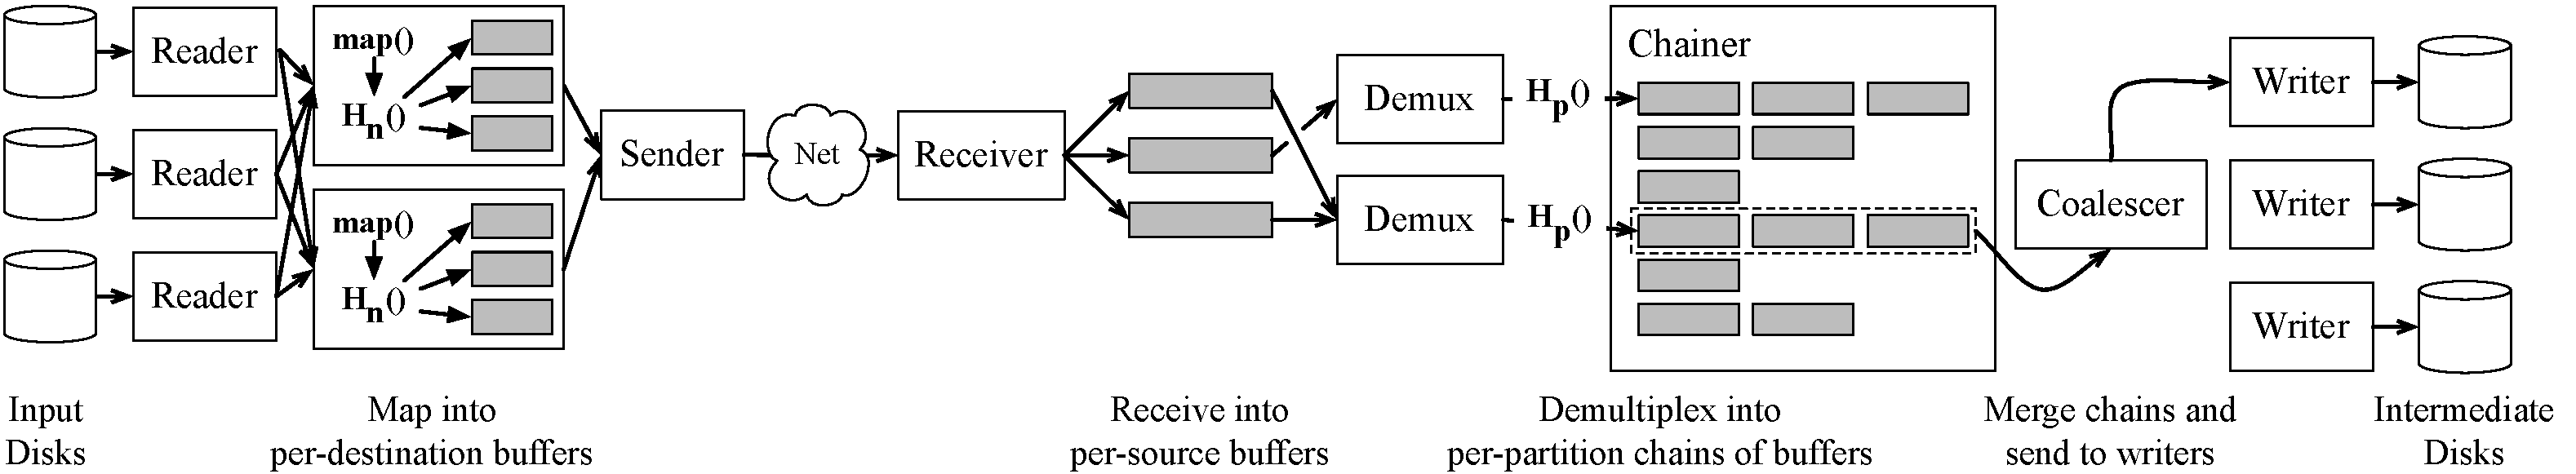
\includegraphics[width=\textwidth]{themis/figures/detailed_phase_one.pdf}
\caption{\label{fig:phase_one} Stages of Phase One (Map/Shuffle) in Themis}
\end{figure*}

Unlike existing MapReduce systems, which executes \map and \reduce tasks
concurrently in waves, Themis implements the MapReduce programming model in
three phases of operation, summarized in Table~\ref{tbl:stages}.  Phase zero,
described in Section~\ref{sec:phase_zero}, is responsible for sampling input
data to determine the distribution of record sizes as well as the distribution
of keys.  These distributions are used by subsequent phases to minimize
partitioning skew.  Phase one, described in Section~\ref{sec:phase_one}, is
responsible for applying the \map function to each input record, and routing
its output to an appropriate partition in the cluster.  This is the equivalent
of existing systems' map and shuffle phases.  Phase two, described in
Section~\ref{sec:phase_two}, is responsible for sorting and applying the
\reduce function to each of the intermediate partitions produced in phase one.
At the end of phase two, the MapReduce job is complete.

\begin{table}
\centering
\caption{\label{tbl:stages} Themis's three stage architecture}
\begin{tabular}{|c|c|c|} \hline
\textbf{Phase} & \textbf{Description} & \textbf{Required?} \\\hline
0 & Skew Mitigation & Optional \\
1 & \texttt{map()} and shuffle & Required \\
2 & sort and \texttt{reduce()} & Required \\\hline
\end{tabular}
\end{table}

Phase one reads each input record and writes each intermediate record exactly
once.  Phase two reads each intermediate partition and writes its corresponding
output partition exactly once.  Thus, Themis has the 2-IO property.

\subsection{Phase One: Map and Shuffle}
\label{sec:phase_one}
\label{sec:map}

Phase one is responsible for implementing both the \map operation as well as
shuffling records to their appropriate intermediate partition.  Each node in
parallel implements the stage graph pipeline shown in
Figure~\ref{fig:phase_one}.

The \Readerbf stage reads records from an input disk and sends them to the
\Mapperbf stage, which applies the \map function to each record.  As the \map
function produces intermediate records, each record's key is hashed to
determine the node to which it should be sent and placed in a
per-destination buffer that is given to the \sender when it is full.  The
\Senderbf sends data to remote nodes using a round-robin loop of short,
non-blocking \texttt{send()} calls.  We call the \Reader to \Sender part of the
pipeline the ``producer-side'' pipeline.

The \Receiverbf stage receives records from remote nodes over TCP using
a round-robin loop of short, non-blocking \texttt{recv()} calls. We implemented
a version of this stage that uses \texttt{select()} to avoid unnecessary
polling, but found that its performance was too unpredictable to reliably
receive all-to-all traffic at 10Gbps. The \receiver places incoming records
into a set of small per-source buffers, and sends those buffers to
the \Demux stage when they become full.

The \Demuxbf stage is responsible for assigning records to partitions.  It
hashes each record's key to determine the partition to which it should be
written, and appends the record to a small per-partition buffer.  When that
buffer becomes full, it is emitted to the \Chainerbf stage, which links buffers
for each partition into separate \emph{chains}.  When chains exceed a
pre-configured length, which we set to 4.5 MB to avoid doing small writes, it
emits them to the \Coalescerbf stage.  The \Coalescerbf stage merges chains
together into a single large buffer that it sends to the \Writerbf stage,
which appends buffers to the appropriate partition file. The combination of the
\Chainer and \Coalescer stages allows buffer memory in front of the \Writer
stage to be allocated to partitions in a highly dynamic and fine-grained way.
We call the \Receiver to \Writer part of the pipeline the ``consumer-side''
pipeline.

A key requirement of the consumer-side pipeline is to perform large, contiguous
writes to disk to minimize seeks and provide high disk bandwidth.  Themis uses
the same node-wide, application-driven disk scheduler used in TritonSort to
ensure that writes are large. We refer the reader to
Section~\ref{sec:tritonsort-disk-scheduler} for details on the disk scheduler's
implementation.

\subsection{Phase Two: Sort and Reduce}
\label{sec:phase_two}
\label{sec:reduce}

\begin{figure}[h]
\centering
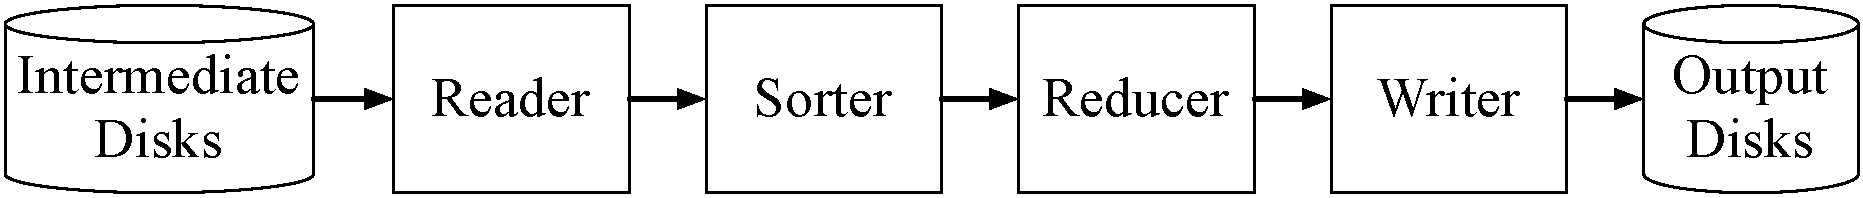
\includegraphics[width=\columnwidth]{themis/figures/phase_two.pdf}
\caption{\label{fig:phase_two} Stages of Phase Two (Sort/Reduce) in Themis}
\end{figure}

By the end of phase one, the map function has been applied to each input
record, and the records have been grouped into partitions and stored on the
appropriate node so that all records with the same key are stored in a single
partition.  In phase two, each partition must be sorted by key, and the \reduce
function must be applied to groups of records with the same key.  The stages
that implement phase two are shown in Figure~\ref{fig:phase_two}.

There is no network communication in phase two, so nodes process their
partitions independently.  Entire partitions are read into memory at once by
the \Readerbf stage. A \Sorterbf stage sorts these partitions by key, keeping
the result in memory.  The \Reducerbf stage applies the \reduce function to all
records sharing a key.  Reduced records are sent to the \Writerbf, which writes
them to disk.

All records with a single key must be stored in the same partition for the
\reduce function to produce correct output. As a result, partitioning skew can
cause some partitions to be significantly larger than others. Themis's memory
management system allows phase two to process partitions that approach the size
of main memory, and its optional skew mitigation phase can reduce partitioning
skew without user intervention. We describe these systems in Sections
\ref{sec:memory} and \ref{sec:phase_zero}, respectively.

A key feature of Themis's \sorter stage is that it can select which sort
algorithm is used to sort a buffer on a buffer-by-buffer basis.  There is a
pluggable \textit{sort strategy} interface that lets developers use different
sorting algorithms; currently quicksort and radix sort are implemented.  Each
sort strategy calculates the amount of scratch space it needs to sort the given
buffer, depending on the buffer's contents and the sort algorithm's space
complexity.  For both quicksort and radix sort, this computation is
deterministic.  In Themis, radix sort is chosen if the keys are all the same
size and the required scratch space is under a configurable threshold;
otherwise, quicksort is used.

\section{Memory Management and Flow Control}
\label{sec:memory}

\begin{table}
  \centering
  \caption{\label{fig:memory-allocator-compare} A comparison of Themis's memory
    allocator implementations.}
  \tabcolsep=0.11cm

  \begin{tabular}{|c|c|c|p{.7cm}|p{.7cm}|p{.7cm}|c|} \hline
    & \multirow{2}{*}{\textbf{TritonSort}} & \multirow{2}{*}{\textbf{Themis}}
    & \multicolumn{3}{c|}{\textbf{Used in Phase}} & \textbf{Subject to} \\\cline{4-6}
    & & & \centering 0 & \centering 1 & \centering 2 & \textbf{deadlock?} \\ \hline
    Pool & $\checkmark$ & $\checkmark$ & \centering $\checkmark$ & \centering $\checkmark$ & & \\\hline
    Quota &  & $\checkmark$ & \centering $\checkmark$ & \centering $\checkmark$ & &  \\\hline
    Constraint &  & $\checkmark$ &  &  & \centering $\checkmark$ & $\checkmark$ \\\hline
  \end{tabular}
\end{table}

Themis relies on a dynamic and flexible memory management system
to partition memory between operators.
Themis's memory manager actually serves two distinct purposes: (1) it
enables resource sharing between operators, and (2) it supports
enforcing back-pressure and flow control.  In the first case, Themis requires
flexible use of memory given our desire to support large amounts of record
size
skew while maintaining the 2-IO property.  In the second case, individual
stages in the Themis pipeline naturally run at different speeds (e.g.,
the network is 10 Gbps, whereas the disk subsystem only supports writing
at approximately 5.5 Gbps), and so back-pressure and flow control are needed
to prevent faster stages from starving slower stages for resources.

Themis supports a single memory allocation interface with pluggable memory
policies.  We first describe the memory allocator's interface, and then
describe the three policies that we have implemented.

\subsection{Memory Allocation Interface}

Worker stages in Themis allocate space for buffers and other necessary
scratch space using a unified and simple memory allocator interface,
shown in Table~\ref{fig:memory-allocator-API}.

\begin{table*}
  \centering
  \caption{\label{fig:memory-allocator-API} A summary of the Themis memory
    allocator API.}
  \resizebox{\columnwidth}{!}{
  \begin{tabular}{|l|l|}
    \hline
    \textbf{Function} & \textbf{Description} \\
    \hline
    \texttt{CallerID \textbf{registerCaller}(Worker worker)} & Register \texttt{worker}
    with the allocator \\
    \hline
    \texttt{void* \textbf{allocate}(CallerID caller, uint64\_t size)} & allocate a
    memory region of \texttt{size} bytes for \texttt{caller} \\
    \hline
    \texttt{void \textbf{deallocate}(void* memory)} & deallocate \texttt{memory} that
    was allocated by this allocator\\
    \hline
  \end{tabular}
  }
\end{table*}

Memory allocators can be assigned on a stage-by-stage basis, but in the current
implementation we assume that memory regions are allocated and deallocated by
the same allocator.  The \texttt{allocate} call blocks until the underlying
memory allocation policy satisfies the allocation, which can be an unbounded
amount of time.  As we will see, this simple mechanism, paired with one of
three memory policies, provides for both resource sharing as well as flow
control.  We now examine each of these polices.

\subsection{Policy 1: Pool-Based Management}

\begin{figure}
  \centering
  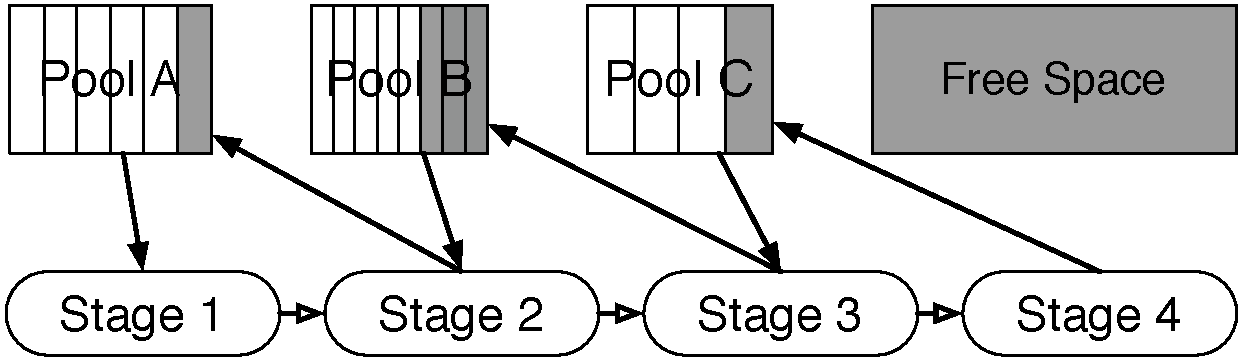
\includegraphics[width=\columnwidth]{themis/figures/pool_based_manager.pdf}
  \caption{\label{fig:memory_allocators:pool} A diagrammatic overview of
    pool-based memory management. Note that memory in each pool is divided into
  fixed-size regions, and that any memory not allocated to pools cannot be
  utilized by stages.}
\end{figure}

The first policy we consider is a ``pool'' memory policy, which is inherited
from TritonSort~\cite{tritonsort}.  A memory pool is a set of pre-allocated
buffers that is filled during startup.  Buffers can be checked out from a pool,
and returned when they are finished being used as illustrated in
Figure~\ref{fig:memory_allocators:pool}.  When a worker tries to check out a
buffer from an empty pool, it blocks until another worker returns a buffer to
that pool.  The pool memory policy has the advantage that all memory allocation
is done at startup, avoiding allocation during runtime.  Through efficient
implementation, the overhead of checking out buffers can be very small.  This
is especially useful for stages that require obtaining buffers with very low
latency, such as the \Receiver stage, which obtains buffers to use in receiving
data from the network.  The \receiver receives uninterpreted bytes from network
sockets into small, fixed-size byte buffers.  These buffers are passed to a
subsequent stage, which converts them into buffers containing complete records.
For this reason, the \receiver can use pool-based management while still
supporting record-size skew.

Pools can be used to provide resource sharing between workers by giving each of
those workers a reference to a single pool.  The producer-consumer relationship
between pairs of stages also provides a form of flow control; the upstream
stage checking out buffers can only produce work at the rate at which the
downstream stage can return them to the pool.  However, pools have several
disadvantages.  First, the buffers in a pool are all fixed-size, and so
the pool memory policy supports very limited amounts of data skew.  By
carving memory up into fixed-size pools, the maximum record size supported by
this policy is limited to the size of the smallest pool.  Additionally, buffer
pools reserve a fixed amount of memory for a particular pair of stages. One
consequence of this is a loss of flexibility; if one stage temporarily needs
more memory than usual (e.g., if it is handling a large record), it cannot
``borrow'' that memory from another stage due to the static partitioning of
memory across pools.

\subsection{Policy 2: Quota-Based Management}

\begin{figure}
  \centering
  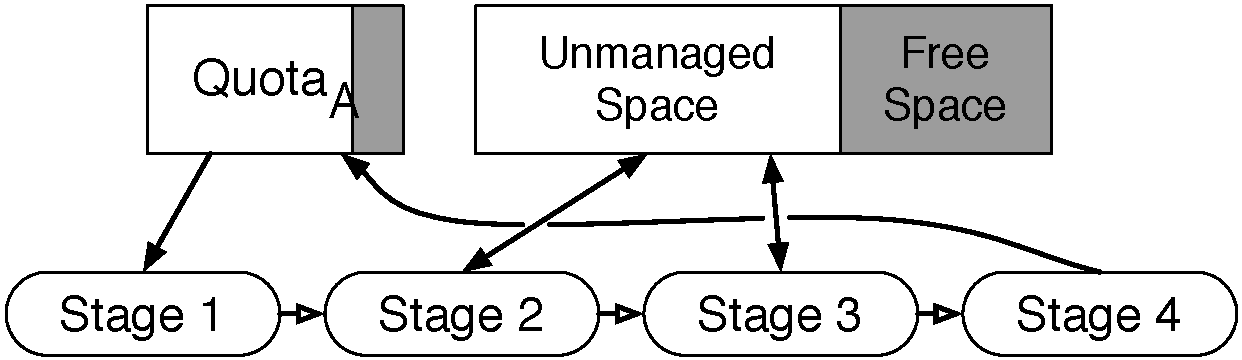
\includegraphics[width=\columnwidth]{themis/figures/quota_based_manager.pdf}
  \caption{\label{fig:memory_allocators:quota} A diagrammatic overview of
    quota-based memory management. In this figure, $Quota_A$ provides a memory
    quota between Stage 1 and Stage 4. Stages 2 and 3 use unmanaged memory
    created with standard \texttt{malloc} and \texttt{free} syscalls.}
\end{figure}

While the pool memory policy is simple, it is quite inflexible, and does not
handle skewed record sizes very well.  The quota-based memory policy is
designed to support more flexible memory allocation while still providing flow
control.  At a high level, the quota policy ensures that stages producing
records do not overwhelm stages that eventually consume them.  For example,
most of our evaluation is \writer limited, and so we want to ensure that the
\receiver stage, which produces records received from the network, does not
overwhelm the \writer stage, which is the bottleneck.

Themis has three such producer-consumer pairs: between the \reader and the
\mapper (with the \mapper acting as the consumer), between the \mapper and the
\sender (with the \mapper acting as the producer), and between the \receiver
and the \writer. The mapper acts as both a consumer and a producer, since it is
the only stage in the phase one pipeline that creates records as directed by
the \map function that were not read by the \reader.

Quotas are enforced by the queues between stages. A quota can be viewed as the
amount of memory that the pipeline between a producer and a consumer can use.
When a producer stage pushes a buffer into the pipeline, the size of that
buffer is debited from the quota.  When a consumer stage consumes that buffer,
the buffer's size is added back to the quota.  If a producer is about to exceed
the quota, then it blocks until the consumer has consumed sufficient
memory. Quota-based allocation is illustrated in
Figure~\ref{fig:memory_allocators:quota}.

Quota-based memory management dramatically reduces the number of variables that
need to be tuned relative to the pool-based memory policy.  One need only
adjust the quota allocations present between pairs of stages, rather than the
capacity of a much larger number of buffer pools.  Additionally, stages that
are not producers and consumers do not need to do any form of coordination,
which makes their memory allocations very fast.

Quota-based management assumes that any scratch space or additional memory
needed by stages between the producer and consumer is accounted for in the
quota.  This is to prevent intermediate stages from exceeding the total amount
of memory, since their memory accesses are not tracked.  It also tacitly
assumes that the size of a buffer being produced cannot exceed the size of the
quota. This is much less restrictive than a pool-based approach, as quotas are
typically several gigabytes.

\subsection{Policy 3: Constraint-Based Management}

\begin{figure}
  \centering
  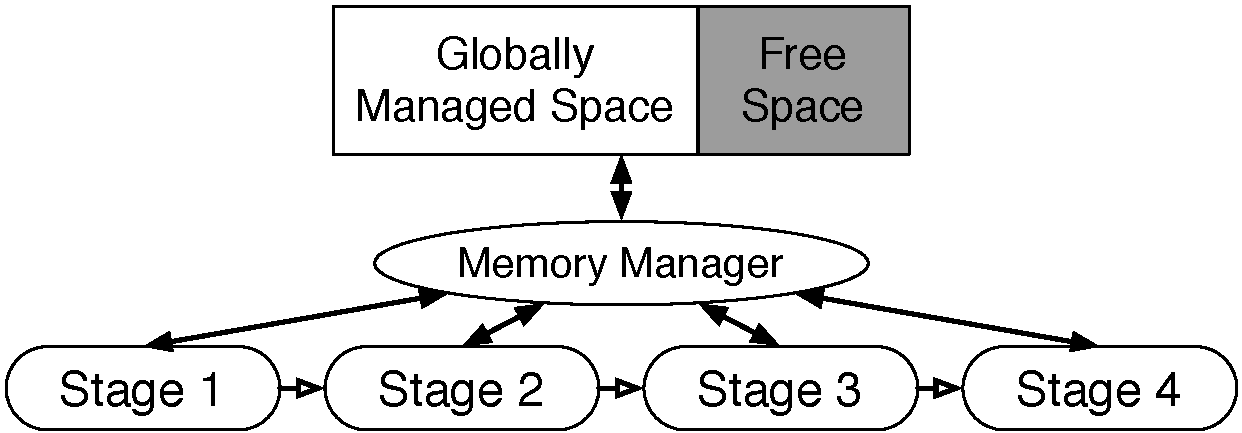
\includegraphics[width=\columnwidth]{themis/figures/constraint_based_manager.pdf}
  \caption{\label{fig:memory_allocators:constraint} A diagrammatic overview of
    constraint-based memory management. All stages' memory requests are
    satisfied by a central memory manager that schedules these requests
    according to the stage graph's structure.}
\end{figure}

In situations where the amount of memory used by stages to process records
cannot be determined in advance, quota-based systems are not ideal for
providing flow control. In these situations, Themis uses a more heavyweight,
constraint-based memory management policy.

In the constraint-based memory policy, the total amount of memory in use by
workers is tracked centrally in the memory allocator. If a worker requests
memory, and enough memory is available, that request is granted immediately.
Otherwise, the worker's request is added to a per-worker queue of outstanding
requests and the worker sleeps on a condition variable until the request can be
satisfied. Constraint-based allocation is illustrated in
Figure~\ref{fig:memory_allocators:constraint}.

When multiple workers have outstanding unsatisfied allocation requests, the
memory allocator prioritizes worker requests based on a worker's distance in
the stage graph to a stage that consumes records.  The producer-side pipeline
measures distance to the \sender stage, and the consumer-side pipeline measures
distance to the \writer stage.  The rationale behind this decision is that
records that are being processed should be completely processed before more
work is admitted. This decision is inspired by work on live-lock prevention in
routers~\cite{ReceiveLivelock}.  In this way, the constraint-based allocator
implements flow control based on the structure of the dataflow graph.

While this system places precise upper bounds on the amount of memory present
in the system, it requires a great deal of coordination between workers, which
requires significant lock contention in our implementation.  In effect, the
reliance on keeping the amount of available memory consistent requires that all
allocation and deallocation requests are processed serially. Hence,
constraint-based memory allocation is useful for situations where the number of
allocation requests being made is relatively small, but the probability of
exceeding available memory in common-case operation is high.  Phase two in
Themis uses constraint-based memory management for precisely these reasons.

In the constraint-based policy, it is possible that certain allocation
interleavings can trigger deadlock.  Predicting whether a general dataflow
system will deadlock is undecidable~\cite{NajjarLeeGao}, and deadlock
prevention requires knowledge of data dependencies between stages that we
deemed too heavyweight. To addressed the problem of deadlocks, Themis provides
a deadlock detector. The deadlock detector periodically probes workers to see
if they are waiting for a memory allocation request to complete. If multiple
probe cycles pass in which all workers are waiting for an allocation or are
idle, the deadlock detector informs the memory allocator that a
deadlock has occurred.  We have not experienced deadlock using the policy
choices described in Table~\ref{fig:memory-allocator-compare} in any of the
MapReduce jobs we have evaluated.  Efficient ways of handling deadlock is the
subject of ongoing work.

In summary, Themis provides a pluggable, policy-driven memory allocation
subsystem that provides for flexible resource sharing between stages and
workers to handle record size skew while also enabling flow control.
% LocalWords:  livelock TritonSort's demux

\section{Skew Mitigation}
\label{sec:phase_zero}

To satisfy the 2-IO property, Themis must ensure that every partition can be
sorted in memory, since an out-of-core sort would induce additional I/Os.  In
addition, to support parallelism, partitions must be small enough that several
partitions can be processed in parallel.  Phase zero is responsible for
choosing the number of partitions, and selecting a partitioning function to
keep each partition roughly the same size.  This task is complicated by the
fact that the data to be partitioned is generated by the \map function.  Thus,
even if the distribution of input data is known, the distribution of
intermediate data may not be known.  This phase is optional: if the user has
knowledge of the intermediate data's distribution, they can specify a custom
partitioning function, similar to techniques used in Hadoop.

Phase zero approximates the distribution of intermediate data by applying the
\map function to a subset of the input.  If the data is homoscedastic, then a
small prefix of the input is sufficient to approximate the intermediate
distribution.  Otherwise, more input data will need to be sampled, or phase
two's performance will decrease.  DeWitt et al.~\cite{ProbabilisticSplitting}
formalize the number of samples needed to achieve a given skew with high
probability; typically we sample 1 GB per node of input data for nodes
supporting 8 TB of input. The correctness of phase two only depends on
partitions being smaller than main memory.  Since our target partition size is
less than 5\% of main memory, this means that a substantial sampling error
would have to occur to cause job failure.  So although sampling does impose
additional I/O over the 2-IO limit, we note that it is a small and constant
overhead.

Once each node is done sampling, it transmits its sample information to a
central coordinator.  The coordinator uses these samples to generate a
partition function, which is then re-distributed back to each node.

\subsection{Mechanism}

On each node, Themis applies the \map operation to a prefix of the records in
each input file stored on that node.  As the \map function produces records,
the node records information about the intermediate data, such as how much
larger or smaller it is than the input and the number of records generated.  It
also stores information about each intermediate key and the associated record's
size.  This information varies based on the sampling policy.  Once the node is
done sampling, it sends that metadata to the coordinator.

The coordinator merges the metadata from each of the nodes to estimate the
intermediate data size.  It then uses this size, and the desired partition
size, to compute the number of partitions.  Then, it performs a streaming
merge-sort on the samples from each node.  Once all the sampled data is sorted,
partition boundaries are calculated based on the desired partition sizes.  The
result is a list of ``boundary keys'' that define the edges of each partition.
This list is broadcast back to each node, and forms the basis of the
partitioning function used in phase one.

The choice of sampling policy depends on requirements from the user,
and we now describe each policy.

\subsection{Sampling Policies}

Themis supports the following sampling policies:

\paragraph{(1) Range partitioning:}
For MapReduce jobs in which the ultimate output of all the reducers must be
totally ordered (e.g., sort), Themis employs a range partitioning sampling
policy.  In this policy, the entire key for each sampled record is
sent to the coordinator.  A downside of this policy is that very large
keys can limit the amount of data that can be sampled because there is
only a limited amount of space to buffer sampled records.

\paragraph{(2) Hash partitioning:} For situations in which total ordering of
\reduce function output is not required, Themis employs hash partitioning.  In
this scheme, a hash of the key is sampled, instead of the keys themselves.
This has the advantage of supporting very large keys, and allowing Themis to
use reservoir sampling~\cite{Vitter:1985:RSR:3147.3165}, which samples data in
constant space in one pass over its input.  This enables more data to be
sampled with a fixed amount of buffer.  This approach also works well for input
data that is already partially or completely sorted because adjacent keys are
likely to be placed in different partitions, which spreads the data across the
cluster.

\section{Evaluation}
\label{sec:eval}

We evaluate Themis through benchmarks of several different MapReduce jobs on
both synthetic and real-world data sets.  A summary of
our results are as follows:

\begin{itemize}
  \item Themis is highly performant on a wide variety of MapReduce jobs, and
    outperforms Hadoop by 3x - 16x on a variety of common jobs.
  \item Themis can achieve nearly the sequential speed of the
  disks for I/O-bound jobs, which is approximately the same rate as TritonSort's
  record-setting performance.
  \item Themis's memory subsystem is flexible, and is able to handle
  large amounts of data skew while ensuring efficient operation.
\end{itemize}

\subsection{Workloads and Evaluation Overview}
\label{sec:methodology}

\begin{table*}
  \centering
  \caption{\label{table:description} A description and table of abbreviations
    for the MapReduce jobs evaluated in this section. Data sizes take into
    account 8 bytes of metadata per record for key and value sizes}
  \resizebox{\columnwidth}{!}{
  \begin{tabular}{|c|p{3.2in}|c|c|c|}
    \hline
    & & \multicolumn{3}{|c|}{\textbf{Data Size}} \\ \cline{3-5}
    \textbf{Job Name}      & \centering \textbf{Description} & Input & Intermediate & Output \\
    \hline
    \hline
    Sort-100G     & Uniformly-random sort, 100GB per node & 2.16TB & 2.16TB & 2.16TB \\
    Sort-500G     & Uniformly-random sort, 500GB per node & 10.8TB & 10.8TB & 10.8TB \\
    Sort-1T       & Uniformly-random sort, 1TB per node & 21.6TB & 21.6TB & 21.6TB\\
    Sort-1.75T    & Uniformly-random sort, 1.75TB per node & 37.8TB & 37.8TB & 37.8TB\\
    \hline
    Pareto-1M     & Sort with Pareto-distributed key/value sizes, $\alpha=1.5$, $x_0=100$ (1MB max key/value size) & 10TB & 10TB & 10TB\\
    Pareto-100M   & Sort with Pareto-distributed key/value sizes, $\alpha=1.5$, $x_0=100$ (100MB max key/value size) & 10TB & 10TB & 10TB\\
    Pareto-500M   & Sort with Pareto-distributed key/value sizes, $\alpha=1.5$, $x_0=100$ (500MB max key/value size) & 10TB & 10TB & 10TB\\
    \hline
    CloudBurst    & CloudBurst (two nodes, performing alignment on
    \texttt{lakewash\_combined\_v2.genes.nucleotide}) & 971.3MB & 68.98GB & 517.9MB\\
    \hline
    PageRank-U    & PageRank (synthetic uniform graph, 25M vertices, ~50K
    random edges per vertex) & 1TB & 4TB & 1TB \\
    PageRank-PL   & PageRank (synthetic graph with power-law vertex in-degree,
    250M vertices)  & 934.7GB & 3.715TB & 934.7GB\\
    PageRank-WEX  & PageRank on WEX page graph & 1.585GB & 5.824GB & 2.349GB\\
    \hline
    WordCount & Count words in text of WEX & 8.22GB & 27.74GB & 812MB \\
    \hline
    n-Gram & Count 5-grams in text of WEX & 8.22GB & 68.63GB & 49.72GB \\
    \hline
    Click-Sessions & Session extraction from 2TB of synthetic click logs & 2TB
    & 2TB & 8.948GB \\
    \hline
  \end{tabular}
}
\end{table*}

We evaluate Themis on the cluster described in
Section~\ref{sec:hardware_architecture}. Each XFS partition is configured with
a single allocation group to prevent file fragmentation across allocation
groups, and is mounted with the \texttt{noatime} flag set. For this evaluation,
all servers were running Linux 2.6.32. Our implementation of Themis is written
in C++ and is compiled with g++ 4.6.2.

To evaluate Themis at scale, we often have to rely on large
synthetically-generated data sets, due to the logistics of obtaining and
storing freely-available, large data sets.  All synthetic data sets are
evaluated on 20 cluster nodes. Non-synthetic data sets are small enough to
be evaluated on a single node.

All input and output data is stored on local disks without using any
distributed filesystem and without replication. We explore Themis's interaction
with distributed storage in Chapter~\ref{chapter:fault_tolerance}.

We evaluate Themis's performance on several different MapReduce jobs. A
summary of these jobs is given in Table~\ref{table:description}, and each job
is described in more detail below.

\subsubsection{Sort}

Large-scale sorting is a useful measurement of the
performance of MapReduce and of data processing systems in general.  During a
sort job, all cluster nodes are reading from disks, writing to disks, and doing
an all-to-all network transfer simultaneously.  Sorting also measures the
performance of MapReduce independent of the computational complexity of the
\map and \reduce functions themselves, since both \map and \reduce functions
are effectively no-ops. We study the effects of both increased data density and
skew on the system using sort due to the convenience with which input data that
meets desired specifications can be generated.  We generate skewed data with a
Pareto distribution.  The record size in generated datasets is limited by a
fixed maximum, which is a parameter given to the job.

\subsubsection{WordCount}

Word count is a canonical MapReduce job. Given a
collection of words, word count's \map function emits \kvpair{word}{1} records
for each word.  Word count's \reduce function sums the occurrences of each word
and emits a single \kvpair{word}{N} record, where N is the number of times
the word occurred in the original collection.

We evaluate WordCount on the 2012-05-05 version of the Freebase Wikipedia
Extraction (WEX)~\cite{wex}, a processed dump of the English version of
Wikipedia. The complete WEX dump is approximately 62GB uncompressed, and
contains both XML and text versions of each page. We run word count on the text
portion of the WEX data set, which is approximately 8.2GB uncompressed.

\subsubsection{n-Gram Count}

 An extension of word count, n-gram count counts the
number of times each group of $n$ words appears in a text corpus. For
example, given ``The quick brown fox jumped over the lazy dog'', 3-gram count
would count the number of occurrences of ``The quick brown'', ``quick brown
fox'', ``brown fox jumped'', etc. We also evaluate n-gram count on the text
portion of the WEX data set.

\subsubsection{PageRank}

PageRank is a graph algorithm that is widely used by
search engines to rank web pages.  Each node in the graph is given an initial
rank. Rank propagates through the graph by each vertex contributing a fraction
of its rank evenly to each of its neighbors.

PageRank's \map function is given a record for each vertex in the graph whose
key is the vertex's ID and whose value is a concatenation of the vertex's
adjacency list and its initial rank. The \map function emits \kvpair{adjacent
  vertex ID}{rank contribution} pairs for each adjacent vertex ID, and also
re-emits the adjacency list so that the graph can be reconstructed. PageRank's
\reduce function adds the rank contributions for each vertex to compute that
vertex's rank, and emits the vertex's existing adjacency list and new rank.

We evaluate PageRank with three different kinds of graphs. The first
(PageRank-U) is a 25M vertex synthetically-generated graph where each vertex
has an edge to every other vertex with a small, constant probability. Each
vertex has an expected degree of 5,000. The second (PageRank-PL) is a 250M
vertex synthetically-generated graph where vertex in-degree follows a power law
distribution with values between 100 and 10,000. This simulates a more realistic
page graph where a relatively small number of pages are linked to
frequently. The third (PageRank-WEX) is a graph derived from page links in the
XML portion of the WEX data set; it is approximately 1.5GB uncompressed and has
~5.3M vertices.

\subsubsection{CloudBurst}

CloudBurst~\cite{cloudburst-bio} is a MapReduce
implementation of the RMAP~\cite{rmap} algorithm for short-read gene alignment,
which aligns a large collection of small ``query'' DNA sequences called
\emph{reads} with a known ``reference'' genome. CloudBurst performs this
alignment using a standard technique called \emph{seed-and-extend}. Both query
and reference sequences are passed to the \map function and emitted as a series
of fixed-size \emph{seeds}. The \map function emits seeds as sequence of
\kvpair{seed}{seed metadata} pairs, where the seed metadata contains
information such as the seed's location in its parent sequence, whether that
parent sequence was a query or a reference, and the characters in the sequence
immediately before and after the seed.

CloudBurst's \reduce function examines pairs of query and reference strings with
the same seed. For each pair, it computes a similarity score of the DNA
characters on either side of the seed using the Landau-Vishkin algorithm for
approximate string matching. The \reduce function emits all query/reference
pairs with a similarity score above a configured threshold.

We evaluate CloudBurst on the lakewash\_combined\_v2 data set from University
of Washington~\cite{cloudburst_uw_data}, which we pre-process using a slightly
modified version of the CloudBurst input loader used in Hadoop.

\subsubsection{Click Log Analysis}

Another popular MapReduce job is analysis of click logs. Abstractly, click logs
can be viewed as a collection of \kvpair{user ID}{timestamp|URL} pairs (where
the \texttt{|} symbol denotes the concatenation of logical fields as part of
the value) indicating which page a user loaded at which time.  We chose to
evaluate one particular type of log analysis task, \emph{session tracking}. In
this task, we seek to identify disjoint ranges of timestamps at least some
number of seconds apart. For each such range of timestamps, we output
\kvpair{user ID}{start timestamp|end timestamp|start URL|end URL} pairs.

The \map function is a pass-through; it simply groups records by user ID. The
\reduce function does a linear scan through records for a given user ID and
reconstructs sessions. For efficiency, it assumes that these records are sorted
in ascending order by timestamp. We describe the implications of this
assumption in the next section.

\subsection{Job Implementation Details}

In this section, we briefly describe some of the implementation details
necessary for running our collection of example jobs at maximum efficiency.

\subsubsection{Combiners}

A common technique for improving the performance of
MapReduce jobs is employing a \emph{combiner}. For example, word count can emit
a single \kvpair{word}{$k$} pair instead of $k$ \kvpair{word}{1}
pairs. Themis supports the use of combiner functions. We opted to implement
combiners within the \mapper stage on a job-by-job basis rather than adding an
additional stage.  Despite what conventional wisdom would suggest, we found
that combiners actually decreased our performance in many cases
because the computational overhead of manipulating large data structures was
enough to make the \mapper compute-bound. The large size of these data
structures is partially due to our decision to run the combiner over an entire
job's intermediate data rather than a small portion thereof to
maximize its effectiveness.

In some cases, however, a small data structure that takes advantage of the
semantics of the data provides a significant performance increase. For example,
our word count MapReduce job uses a combiner that maintains a counter for the
top 25 words in the English language.  The combiner updates the appropriate
counter whenever it encounters one of these words rather than creating an
intermediate record for it.  At the end of phase one, intermediate records are
created for each of these popular words based on the counter values.

\subsubsection{Improving Performance for Small Records}

The \map functions in our first implementations of word count and n-gram count
emitted \kvpair{<word/n-gram}{1} pairs. Our implementations of these \map
functions emit \kvpair{hash(word)}{1|word} pairs instead because the resulting
intermediate partitions are easier to sort quickly because the keys are all
small and the same size.

\subsubsection{Secondary Keys}

A na\"{\i}ve implementation of the session extraction job sorts records for a
given user ID by timestamp in the \reduce function. We avoid performing two
sorts by allowing the \Sorter stage to use the first few bytes of the value,
called a \emph{secondary key}, to break ties when sorting. For example, in the
session extraction job the secondary key is the record's timestamp.

\subsection{Performance}

We evaluate the performance of Themis in two ways. First, we compare
performance of the benchmark applications to the cluster's hardware
limits. Second, we compare the performance of Themis to that of Hadoop on two
benchmark applications.

\subsubsection{Performance Relative to Disk Speeds}

\begin{figure}
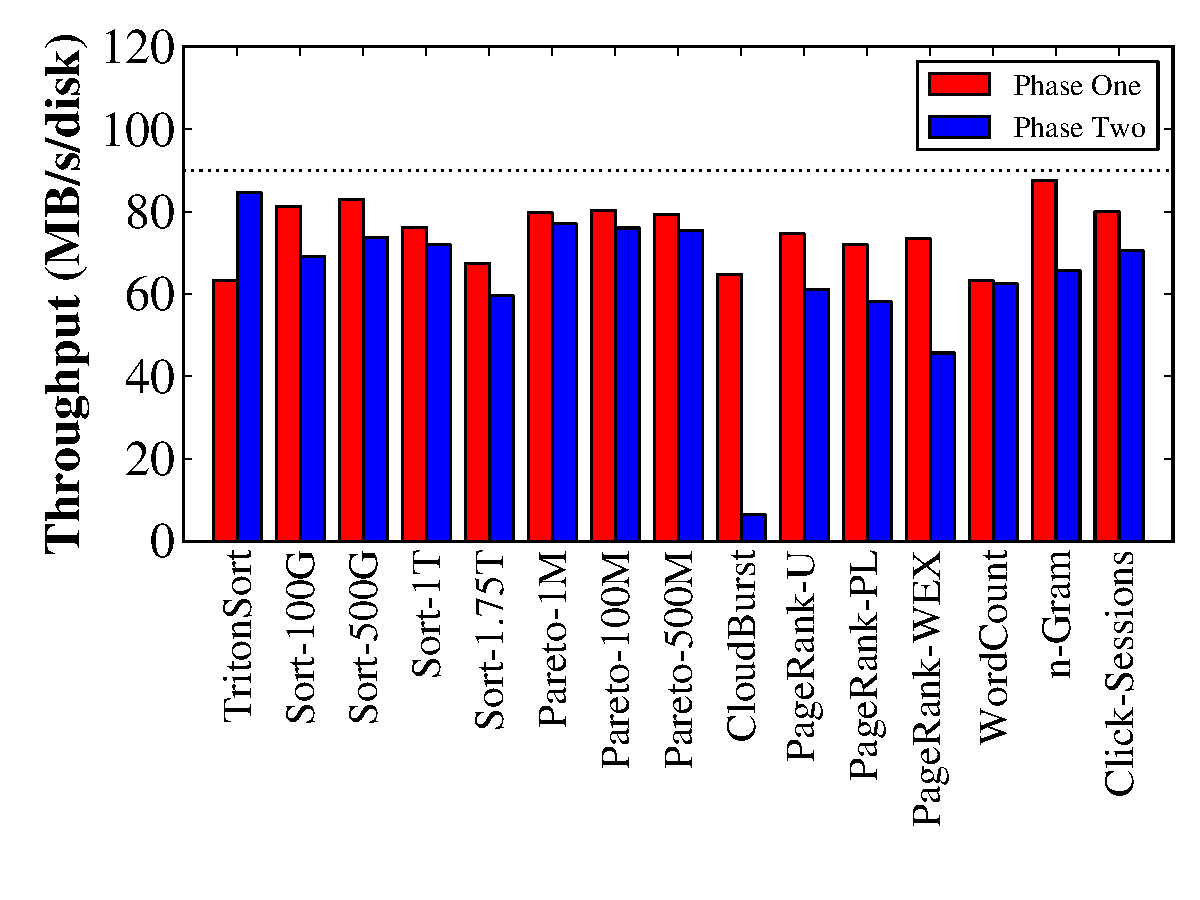
\includegraphics[width=\columnwidth]{themis/graphs/performance.pdf}
\caption{\label{fig:performance} Performance of evaluated MapReduce
  jobs. Maximum sequential disk throughput of approximately 90 MB/s is shown as
  a dotted line. Our TritonSort record from 2011 is shown on the left for
  comparison.}
\end{figure}

The performance of Themis on the benchmark MapReduce jobs is shown in
Figure~\ref{fig:performance}. Performance is measured in terms of
\emph{MB/s/disk} in order to provide a relative comparison to the hardware
limitations of the cluster. The 7200 RPM drives in the cluster are capable of
approximately 90 MB/s/disk of sequential write bandwidth, which is shown as a
dotted line in the figure. A job running at 90 MB/s/disk is processing data as
fast as it can be written to the disks.

Most of the benchmark applications run at near maximum speed in both
phases. CloudBurst's poor performance in phase two is due to the
computationally intensive nature of its \reduce function, which is unable to
process records fast enough to saturate the disks. More CPU cores are needed to
drive computationally intensive applications such as CloudBurst at maximum
speed in both phases. Notice however that CloudBurst is still able to take
advantage of our architecture in phase one.

We have included TritonSort's performance on the Indy 100TB sort benchmark for
reference. TritonSort's 2011 Indy variant runs a much simpler code base than
Themis. We highlight the fact that Themis's additional complexity and
flexibility does not impact its ability to perform well on a variety of
workloads. Our improved performance in phase one relative to TritonSort at
scale is due to a variety of internal improvements and optimizations made to
the codebase in the intervening period, as well as the improved memory
utilization provided by moving from buffer pools to dynamic memory
management. Performance degradation in phase two relative to TritonSort is
mainly due to additional CPU and memory pressure introduced by the \Reducer
stage.

\subsubsection{Comparison with Hadoop}

\begin{table}
  \centering
  \caption{\label{table:hadoop} Performance comparison of Hadoop and Themis.}
  \begin{tabular}{|c|c|c|c|}
    \hline
     & \multicolumn{2}{|c|}{\textbf{Running Time}} &
     \\
    \cline{2-3}
    \textbf{Application} & Hadoop & Themis & \textbf{Improvement}\\
    \hline
    Sort-500G & 28881s & 1789s & 16.14x \\
    CloudBurst & 2878s & 944s & 3.05x \\
    \hline
  \end{tabular}
\end{table}

We evaluate Hadoop version 1.0.3 on the Sort-500G and CloudBurst
applications. We started with a configuration based on the configuration used
by Yahoo! for their 2009 Hadoop sort record~\cite{terasort}. We optimized
Hadoop as best we could, but found it difficult to get it to run many large
parallel transfers without having our nodes blacklisted for running out of
memory.

The total running times for both Hadoop and Themis are given in
Table~\ref{table:hadoop}. I/O-bound jobs such as sort are able to take full
advantage of our architecture, which explains why Themis is more than a factor
of 16 faster. As explained above, CloudBurst is fundamentally compute-bound,
but the performance benefits of the 2-IO property allow the Themis
implementation of CloudBurst to outperform the Hadoop implementation by a
factor of 3.

\subsection{Memory Management}

In this section, we evaluate the performance of our different memory allocation
policies. We also show that our allocation system is robust in the face of
transient changes in individual stage throughputs.

\subsubsection{Memory Allocator Performance}

\begin{figure}
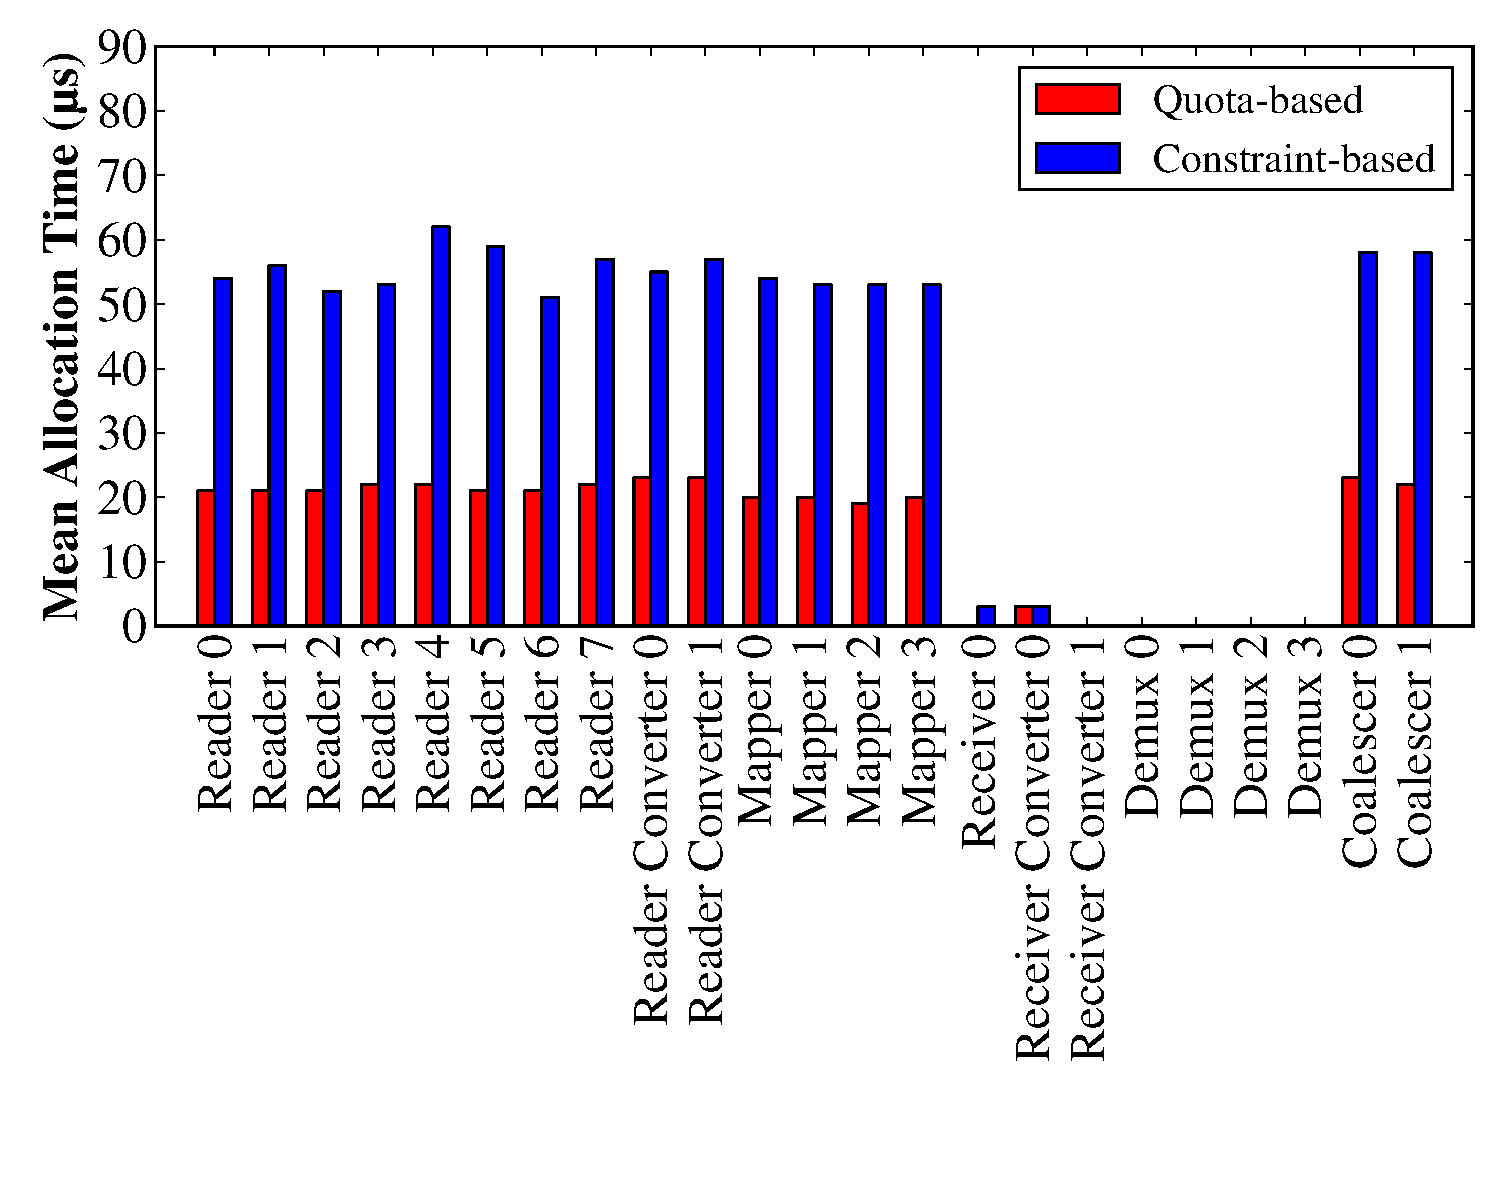
\includegraphics[width=\columnwidth]{themis/graphs/allocation_time_means.pdf}
\caption{\label{fig:allocation_time_means} Effects of allocation policy on mean
allocation times across workers}
\end{figure}

\begin{table}
  \centering
  \caption{\label{table:allocator_end_to_end_performance} Performance of
    allocation policies}
  \begin{tabular}{|c|c|}
    \hline
    \textbf{Allocation Policy} & \textbf{Phase One Throughput} \\
    \hline
    Constraint-Based & 84.90 MBps/disk \\
    Quota-Based & 83.11 MBps/disk \\
    \hline
  \end{tabular}
\end{table}

We examine both the individual allocation times of our different memory
allocation policies and their end-to-end performance.  We evaluate the
performance on phase one of a 200GB, 1-node sort
job. Table~\ref{table:allocator_end_to_end_performance} shows that phase one's
throughput is essentially unaffected by the choice of allocator policy in this
particular instance. These performance numbers can be explained by looking at
the mean allocation time for each worker in the
system. Figure~\ref{fig:allocation_time_means} shows that while the
constraint-based allocator is more than twice as slow as the quota-based
allocator, the absolute allocation times are both measured in tens of
microseconds, which is negligible compared to time taken to actually do useful
work.

However, the results above only hold in the case where the constraint-based
allocator does not deadlock. While we never experienced deadlock in phase two,
we found it was quite easy to construct situations in which phase one
deadlocked. For example, the exact same experiment conducted on a slightly
larger data set causes deadlock in phase one with the constraint-based
allocator.

The performance results in Figure~\ref{fig:performance} demonstrate the
constraint-based allocation policy performs well in phase two.  Because phase
two handles entire intermediate partitions in memory, its allocations are
orders of magnitude larger than those in phase one. This dramatically increases
the likelihood that a single memory request is larger than one of the phase's
quotas.

\subsubsection{Robustness of the Quota-Based Memory Allocation Policy}

\begin{figure}
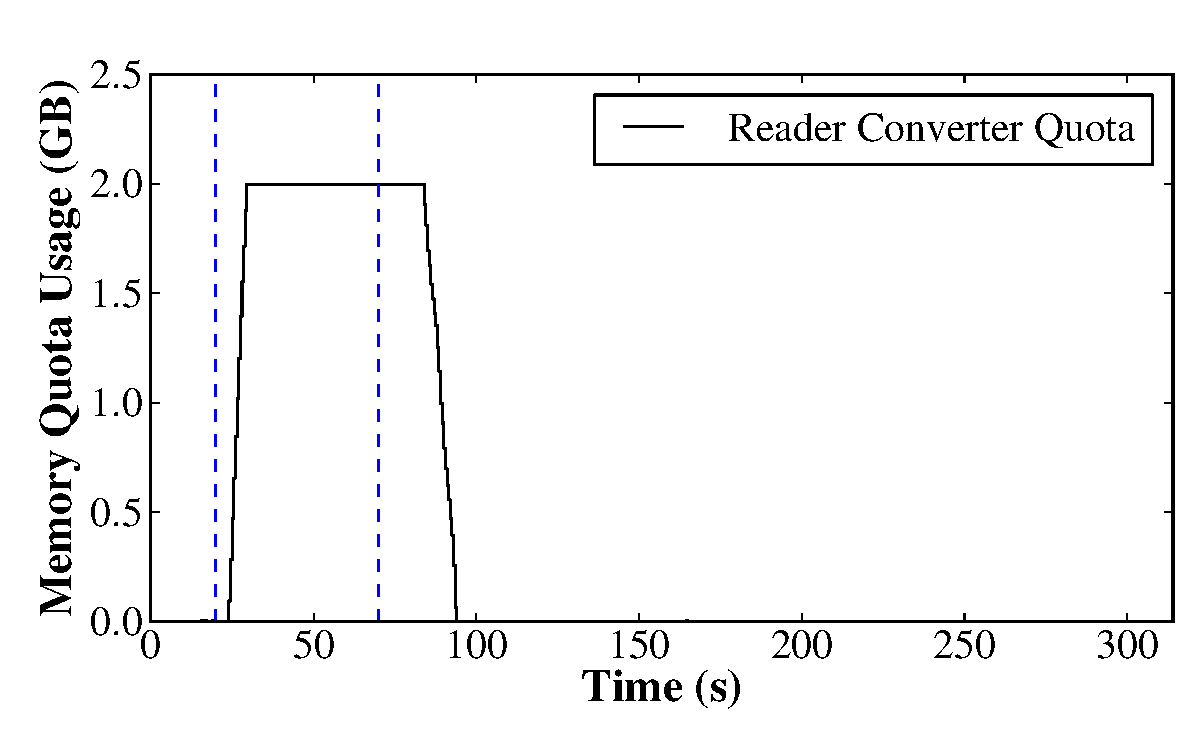
\includegraphics[width=\columnwidth]{themis/graphs/reader_converter_quota_slow_network.pdf}
\caption{\label{fig:reader_converter_quota_slow_network} Memory quota usage of
  the Reader Converter stage. The network was made artificially slow in the
  time period designated by the dashed lines.}
\end{figure}

We evaluate the robustness of the quota-based memory allocator by artificially
slowing down the network for a period of time. We observe the effect on the
total quota usage of a stage in the pipeline. Figure
\ref{fig:reader_converter_quota_slow_network} shows that the Reader Converter's
quota usage spikes up to its limit of 2GB in response to a slow network and
then returns back to a steady state of near 0. A slow network means that stages
upstream of the network are producing data faster than the network can transmit
data. This imbalance leads to data backing up in front of the
network. In the absence of the quota allocation policy, this data backlog grows
unbounded.

\subsection{Skew Mitigation}

\begin{figure}
  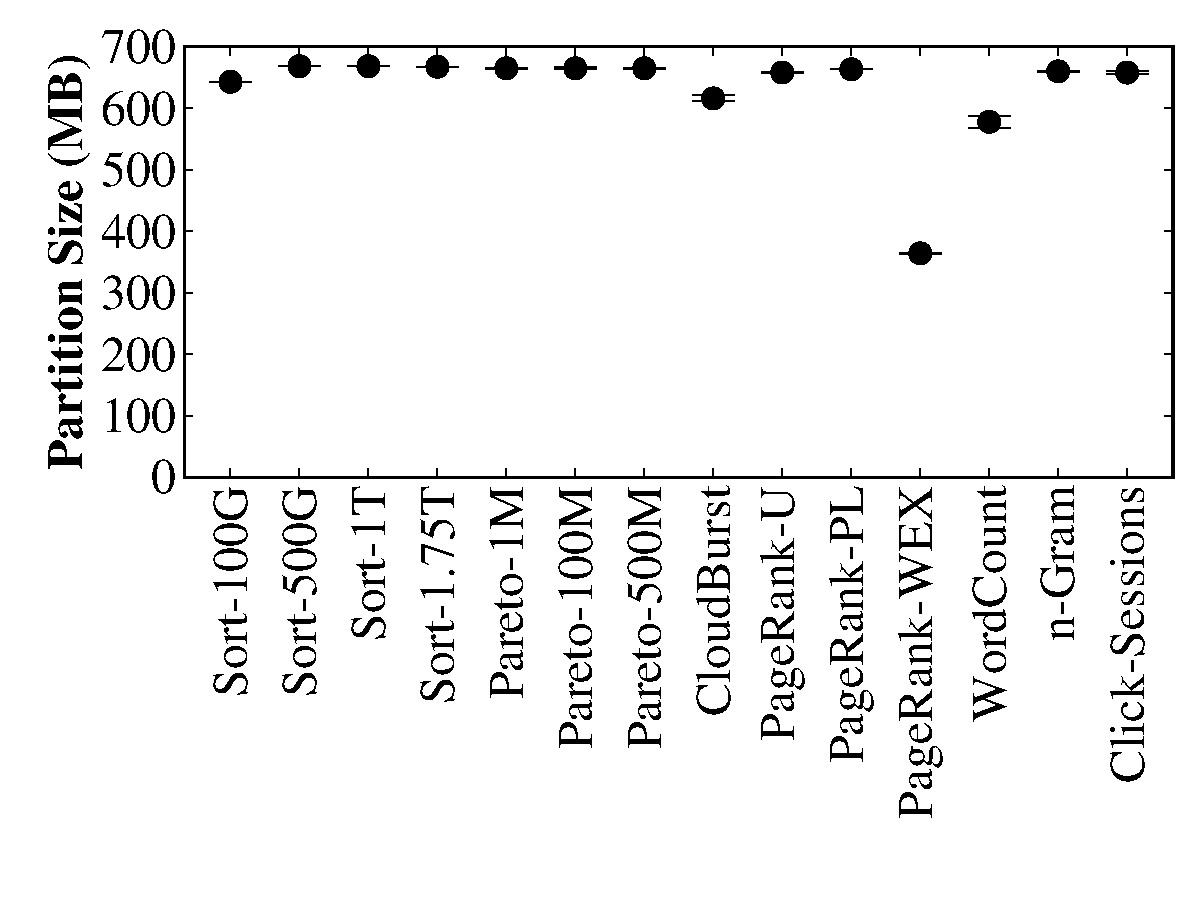
\includegraphics[width=\columnwidth]{themis/graphs/ld_sizes_plot.pdf}
  \caption{\label{fig:ld_sizes} Partition sizes for various Themis
    jobs. Error bars denoting the 95\% confidence intervals are hard to see
    due to even partitioning.}
\end{figure}

Next, we evaluate Themis's ability to handle skew by observing the sizes of
the intermediate data partitions created in phase one.
Figure~\ref{fig:ld_sizes} shows the partition sizes produced by Themis on the
evaluated applications. The error bars denoting the 95\% confidence intervals
are small, indicating that all partitions are nearly equal in size. This is
unsurprising for applications with uniform data, such as sort. However, Themis
also achieves even partitioning on very skewed data sets, such as
Pareto-distributed sort, PageRank, and WordCount. PageRank-WEX has fairly small
partitions relative to the other jobs because its intermediate data size is not
large enough for phase zero to create an integer number of partitions with the
desired size.

\subsection{Write Sizes}

\begin{figure}
  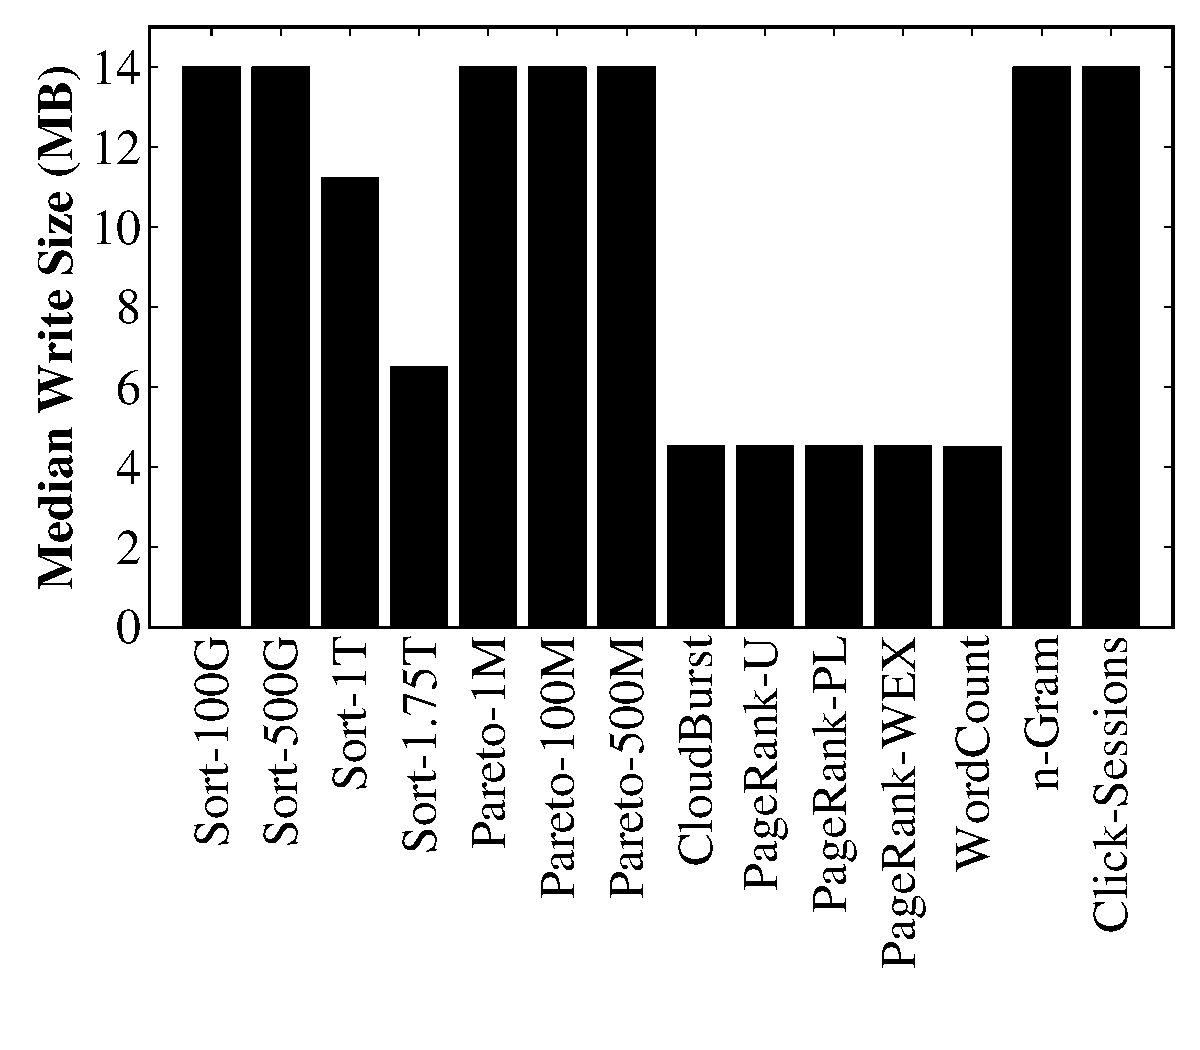
\includegraphics[width=\columnwidth]{themis/graphs/write_sizes_median_bars.pdf}
  \caption{\label{fig:write_sizes} Median write sizes for various Themis jobs}
\end{figure}

One of primary goals of phase one is to do large writes to each partition to
avoid unnecessary disk seeks.  Figure~\ref{fig:write_sizes} shows the median
write sizes of the various jobs we evaluated.  For jobs like Sort and n-Gram
where the \map function is extremely simple and \mappers can map data as fast
as \readers can read it, data buffers up in the \Chainer stage and all writes
are large. As the amount of intermediate data per node grows, the size of a
chain that can be buffered for a given partition decreases, which fundamentally
limits the size of a write. For example, Sort-1.75T writes data to 2832
partitions, which means that its average chain length is not expected to be
longer than about 5 MB given a \receiver memory quota of 14GB; note, however,
that the mean write size is above this minimum value, indicating that the
\writer is able to take advantage of temporary burstiness in activity for
certain partitions.  If the stages before the \Writer stage cannot quite
saturate it (such as in WordCount, CloudBurst and PageRank), chains remain
fairly small. Here the minimum chain size of 4.5 MB ensures that writes are
still reasonably large. In the case of PageRank-WEX, the data size is
too small to cause the chains to ever become very large.

\section{Conclusions}
\label{themis:sec:conclusions}

Many MapReduce jobs are I/O-bound, and so minimizing the number of I/O
operations is critical to improving their performance.  In this work, we
present Themis, a MapReduce implementation that meets the 2-IO property,
meaning that it issues the minimum number of I/O operations for jobs large
enough to exceed memory.  To avoid materializing intermediate results, Themis
foregoes task-level fault tolerance, relying instead on job-level fault
tolerance. Since the 2-IO property prohibits it from spilling records to disk,
Themis must manage memory dynamically and adaptively. To ensure that writes to
disk are large, Themis adopts a centralized, per-node disk scheduler that
batches records produced by different \mappers.

There exist a large and growing number of clusters that can process
petabyte-scale jobs, yet are small enough to experience a qualitatively lower
failure rate than warehouse-scale clusters.  We argue that these deployments
are ideal candidates to adopt more efficient implementations of MapReduce,
which result in higher overall performance than more pessimistic
implementations.  Themis has been able to implement a wide
variety of MapReduce jobs at nearly the sequential speed of the underlying
storage layer, and is on par with TritonSort's record sorting performance.

\section{Acknowledgments}
\label{sec:ack}

The authors wish to thank Kenneth Yocum for his valuable input, as well as
Mehul Shah and Chris Nyberg for their input on Themis's approach to
sampling.  This work was sponsored in part by NSF Grants CSR-1116079 and MRI
CNS-0923523, as well as through donations by Cisco Systems and a NetApp Faculty
Fellowship.

Chapter~\ref{chapter:themis} contains material as it appears in the Proceedings
of the ACM Symposium on Cloud Computing (SoCC) 2012. ``Themis: An I/O-Efficient
MapReduce''. Rasmussen, Alexander; Conley, Michael; Kapoor, Rishi; Lam, Vinh
The; Porter, George; Vahdat, Amin. The dissertation author was the primary
investigator and author of this paper.



\def\themis{Themis\xspace}

\chapter{I/O-Efficient Fault Tolerance}
\label{chapter:fault_tolerance}

A key requirement when building scale-out data processing architectures is
allowing them to recover from failures in a manner that is transparent to the
end user. Traditional MapReduce implementations provide fault tolerance by
materializing intermediate data to disk on both sides of a network
transfer. This increases the amount of disk I/O that each MapReduce job must
perform, which fundamentally limits the performance of I/O-bound workloads.

In this chapter, we argue that small and medium clusters -- on which MapReduce
is commonly deployed, and where the likelihood of a failure during a job is low
relative to large-scale clusters -- can benefit from more optimistic forms of
fault tolerance for which the common-case overhead is far lower than
traditional approaches. In particular, we explore the implications of the
job-level fault tolerance approach adopted by Themis in the previous chapter,
and describe an alternative fault tolerance method for Themis that leverages
prior work in scan sharing and eager record-level provenance.


\section{Introduction}

A key requirement and challenge in building scale-out data processing
architectures is allowing them to recover from failures without burdening the
programmer. MapReduce traditionally provides fault tolerance by splitting the
execution of the \map and \reduce functions into a collection of idempotent
\emph{tasks}. Each map task operates over a portion of the input, while each
reduce task operates over records produced by the \map function with a
particular set of keys. When a task fails, it is simply re-executed. We refer
to this method of fault tolerance as ~\emph{task-level fault tolerance}.

A key benefit of this fault tolerance technique is that it is
\emph{proportional}. Generally speaking, this means that the amount of
additional work required to recover from a failure is proportional to the size
of that failure. Proportional fault tolerance techniques work extremely well on
clusters containing thousands of nodes, because failures in those environments
are extremely common and the relative size of each individual failure is
small~\cite{jeff-dean-talk}.

In MapReduce's case, however, proportional fault tolerance comes with a
significant cost; map tasks must materialize their output to their local disks
before transferring that output to reduce tasks. These materializations are
required because, in general, each reduce task needs some of the records
produced by every map task in order to run. Were map tasks to send their
outputs to reduce tasks directly, the loss of the node on which a reduce
task runs would require that map tasks re-compute all data sent to that
task. In I/O-bound applications, the extra materializations required by
task-level fault tolerance can negatively
affect performance.

Many modern MapReduce clusters are ``dense'', in the sense that they pack a
large amount of storage, compute, and network bandwidth into a small number of
racks of servers. In this chapter, we show that in these ``dense'' clusters,
the additional I/O necessitated by task-level fault tolerance often leads to
lower overall job throughput than simply re-running a job if a failure
occurs.

The more optimistic \emph{job-level fault tolerance} employed by \themis in the
previous chapter allows \themis to perform much more aggressive operator
pipelining than task-level fault tolerance can achieve while still maintaining
the 2-IO property. However, job-level fault tolerance precludes running jobs
that take longer than the cluster MTTF to complete, preventing large clusters
(or unusually failure-prone small ones) from running some jobs.  To mitigate
this problem, we present a fault tolerance approach that provides proportional
recovery without imposing additional intermediate data materialization during
failure-free execution. Our main goal in designing this fault tolerance scheme
is to perform as little additional I/O as possible both in common case
operation and during recovery from failure.

Our contributions are as follows:

\begin{enumerate}
  \item We explore the tradeoffs of different levels of fault tolerance in
    ``dense'' clusters.
  \item We modify \themis to allow it to run multiple jobs concurrently, using
    scan sharing~\cite{nova, qptmd, coscan} to reduce the amount of I/O
    required for each job.
  \item Leveraging this multi-tenant capability, we present a fault tolerance
    mechanism that composes previously known techniques to reduce the amount of
    additional I/O needed for recovery at the expense of additional redundant
    computation.
  \item We show how this fault tolerance mechanism can be used to provide
    proportional recovery both from failures of a single disk and an entire
    node. When scan sharing, an eight-node \themis cluster can recover from a
    disk failure with under 5\% overhead.
  \item We compare this approach to approaches based on record-based provenance
    information.
\end{enumerate}

\section{Motivation}
\label{sec:motivation}
\label{sec:assumptions}

In this section, we summarize the argument for replacing task-level fault
tolerance as MapReduce's fault tolerance scheme for ``dense'' clusters. We then
provide an overview of alternative fault approaches used by current data
processing systems.

\subsection{Fault Tolerance for ``Dense'' Clusters}
\label{sec:ft_provenance}

\begin{figure*}[t]
\centering
\begin{subfigure}[t]{0.47\textwidth}
  \centering
  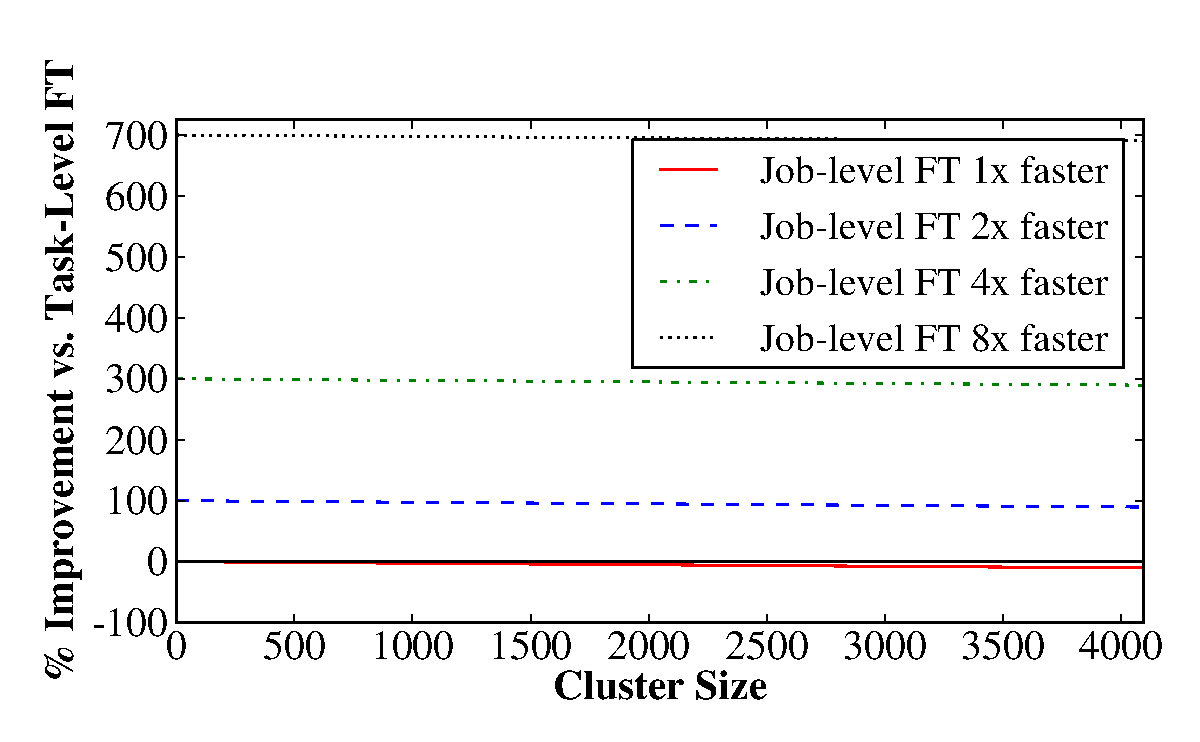
\includegraphics[width=\textwidth]{themis/graphs/analytical_failure_motivation/factor_5min}
  \caption{\label{fig:ft_motivation5} 5-minute job}
\end{subfigure}
\begin{subfigure}[t]{0.47\textwidth}
\centering
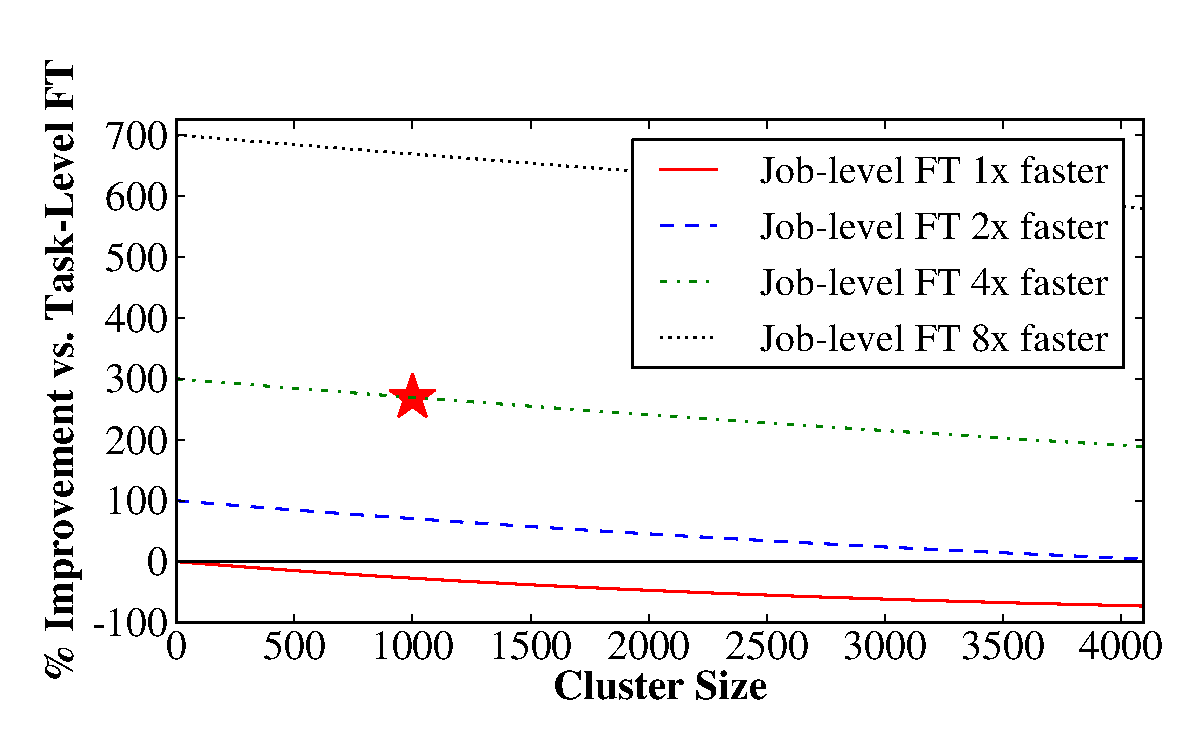
\includegraphics[width=\textwidth]{themis/graphs/analytical_failure_motivation/factor_60min}
\caption{\label{fig:ft_motivation60} 1-hour job (see text below for explanation of marked point)}
\end{subfigure}
\begin{subfigure}[t]{0.47\textwidth}
\centering
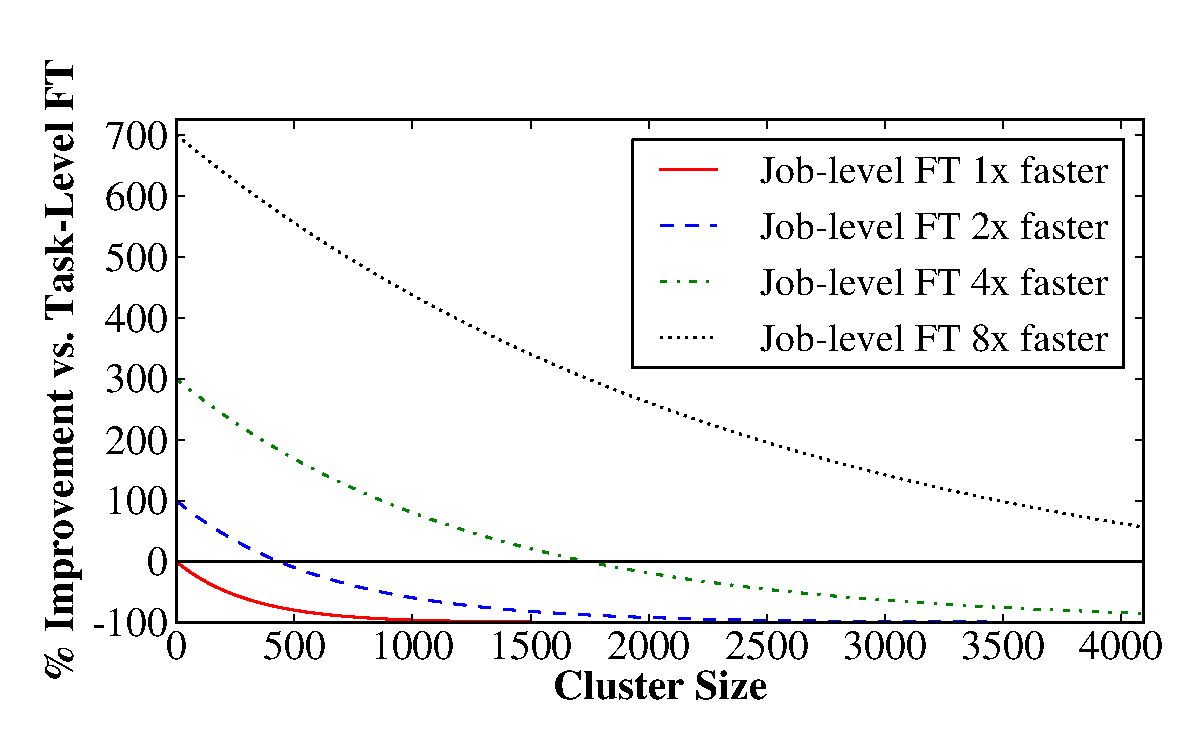
\includegraphics[width=\textwidth]{themis/graphs/analytical_failure_motivation/factor_600min}
\caption{\label{fig:ft_motivation600}10-hour job}
\end{subfigure}
\caption{\label{fig:ft_motivation} A lower-bound of the expected benefit of
  job-level fault tolerance for varying cluster sizes, given
  that an error-free execution of a job with task-level fault tolerance takes
  five minutes (\subref{fig:ft_motivation5}), an hour (\subref{fig:ft_motivation60}),
  or ten hours (\subref{fig:ft_motivation600}) to complete.}
\end{figure*}

Much of MapReduce's architecture is based on the assumption that it is running
on a very large cluster of unreliable machines.  However, a large number of
``Big Data'' clusters do not approach the size of warehouse-scale data centers
like those at Google and Microsoft because moderately-sized clusters (10s of
racks or fewer) are increasingly able to support important real-world problem
sizes.  The storage capacity and number of CPU cores in commodity servers are
both increasing rapidly.  In Cloudera's reference system
design~\cite{ClouderaDellHadoopPlatform}, in which each node has 16 or more
disks, a petabyte worth of 1TB drives fits into just over three racks, or about
60 nodes.  Coupled with the emergence of affordable 10 Gbps Ethernet at the end
host and increasing bus speeds, data can be packed more densely than ever
before while keeping disk I/O as the bottleneck resource.  This implies that
fewer servers are required for processing large amounts of data for I/O-bound
workloads.  We now consider the implications of this increased density on fault
tolerance.

Job-level fault tolerance allows for much more aggressive operator pipelining
than task-level fault tolerance can achieve while still maintaining the 2-IO
property.  However, it is not self-evident that the overhead of re-executing
failed jobs does not cancel any performance gained by this aggressive
pipelining.  In this section, we show not only that job-level fault tolerance
is a feasible approach for moderately-sized clusters, but also that there are
significant potential performance benefits for using job-level fault tolerance
in these environments.

\begin{table}
\centering
\caption{\label{tbl:googleMttf} Component-level failure rates
observed in a Google data center as reported
in~\cite{google-availability:osdi10}.}
\begin{tabular}{|c|c|} \hline
\textbf{Component} & \textbf{Failure rates}\\\hline
Node & 4.3 months \\
Disk & 2-4\% annualized\\
Rack & 10.2 years \\\hline
\end{tabular}
\end{table}

Understanding the expected impact of failures is critical to choosing the
appropriate fault tolerance model.  MapReduce was designed for clusters of many
thousands of machines running inexpensive, failure-prone commodity
hardware~\cite{mapreduce}.  For example, Table~\ref{tbl:googleMttf} shows
component-level mean-time to failure (MTTF) statistics in one of Google's data
centers~\cite{google-availability:osdi10}. Google's failure statistics are
corroborated by similar studies of hard
drive~\cite{DBLP:conf/fast/PinheiroWB07,Schroeder:2007:UDF:1288783.1288785} and
node~\cite{DBLP:conf/nsdi/NathYGS06, Schroeder:2010:LSF:1916484.1916652}
failure rates.

\subsection{Modeling Node Failure Rates}

At massive scale, there is a high probability that some portion of the cluster
will fail during the course of a job.  To understand this probability, we
employ a simple model~\cite{sysreliability}, shown in
Equation~\ref{eqn:jobfailure}, to compute the likelihood that a node in a
cluster of a particular size will experience a failure during a job:

\begin{equation}
P(N, t, MTTF) = 1 - e^{-N \cdot t / MTTF}
\label{eqn:jobfailure}
\end{equation}

The probability of a failure occurring in the next $t$ seconds is
a function of (1) the number of nodes in the cluster, $N$, (2) $t$, and (3) the
mean time to failure of each node, $MTTF$, taken from the node-level failure
rates in Table~\ref{tbl:googleMttf}.  This model assumes that nodes fail with
exponential (Pareto) probability, and we simplify our analysis by considering
node failures only.  We do this because disk failures can be made rare by using
node-level mechanisms (i.e., RAID), and correlated rack failures are likely to
cripple the performance of a cluster with only a few racks.

Based on the above model, in a 100,000 node data center, there is a 93\% chance
that a node will fail during any five-minute period. On the other hand, in a
moderately-sized cluster (e.g., 200 nodes, the average Hadoop cluster size as
reported by Cloudera), there is only a 0.53\% chance of encountering a node
failure during a five-minute window, assuming the MTTF rates in
Table~\ref{tbl:googleMttf}.

This leads to the question of whether smaller deployments benefit from
job-level fault tolerance, where if any node running a job fails the entire job
restarts.  Intuitively, this scheme will be more efficient overall when
failures are rare and/or jobs are short.

\subsection{Modeling Expected Job Completion Time}

Let $T$ be the job's duration and $MTTF$ be the mean time to failure of the
cluster. In our model, failure occurs as a Poisson process. We compute the
expected running time of a failed job (denoted $T_F$) as follows:

\vspace{-4mm}

\begin{eqnarray}
T_{F} &=& \int_{0}^{T} t \cdot \frac{1}{MTTF} e^{-\frac{t}{MTTF}} dt \notag \\
      &=& \left[- t e^{-\frac{t}{MTTF}} - MTTF \cdot e^{-\frac{t}{MTTF}}\right]_{t = 0}^{t = T} \notag \\
      &=& MTTF - (T + MTTF) e^{-\frac{T}{MTTF}}
\label{eqn:T_F}
\end{eqnarray}

Therefore, if the job duration $T$ is much larger than the MTTF of the cluster
($T \gg MTTF$), Equation~\ref{eqn:T_F} implies that $T_F \approx MTTF$, and we
expect the job to fail. On the other hand, if $T \ll MTTF$,
Equation~\ref{eqn:T_F} implies that $T_F \approx T$, and we expect the job to
succeed.

Having modeled the running time of a failed job, we can now derive a model for
overall job completion time. Let $p$ denote the probability of failure in a
single Themis job.  Let $T$ denote the running time of the job when there are
no failures.

Consider a situation in which the job fails during the first $(n-1)$ trials and
completes in the $n^{th}$ trial. The probability of this event is $p^{n-1} (1 -
p)$.  Note that a successful trial takes time $T$ and a failed trial takes time
$T_F$.  To simplify our notation, let $\alpha = T_F / T$ be the fraction of its
successful runtime the failed job spent running.  Then the total running time
in this case is
\[(n-1) \alpha T + T = ((n-1) \alpha + 1) T.\]

By considering such an event for all possible values of $n$, we get the
expected running time to completion for the job:

\vspace{-4mm}

\begin{eqnarray}
   S(p, T) &=& \sum_{n=1}^{\infty} ((n-1) \alpha + 1) T \cdot p^{n-1}(1-p)  \notag \\
           &=& T(1-p) \sum_{n=1}^{\infty} \left(\alpha n p^{n-1} + (1-\alpha) p^{n-1}\right)  \notag \\
           &=& T(1-p) \left(\alpha \sum_{n=1}^{\infty} n p^{n-1} + (1 - \alpha) \sum_{n=1}^{\infty} p^{n-1}\right) \notag \\
           &=& T(1-p) \left(\alpha \frac{1}{(1-p)^2} + (1 - \alpha) \frac{1}{1-p}\right) \notag \\
           &=& T \left(\alpha \frac{p}{1-p} + 1\right)
\label{eqn:job}
\end{eqnarray}

Hence, we can model the expected completion time of a job $S(p,T)$ as:

\begin{equation}
S(p,T) = T\left(\frac{p}{1 - p} + 1\right)
\label{eqn:expectedjobtime}
\end{equation}

where $p$ is the probability of a node in the cluster failing, and $T$ is the
runtime of the job.  This estimate is pessimistic, in that it assumes that jobs
fail just before the end of their execution.

By combining equations~\ref{eqn:jobfailure} and \ref{eqn:expectedjobtime}, we
can compute the expected benefit--or penalty--that we get by moving to
job-level fault tolerance.  Modeling the expected runtime of a job with
task-level fault tolerance is non-trivial, so we instead compare to an
error-free baseline in which the system's performance is not affected by node
failure.  This comparison underestimates the benefit of job-level fault
tolerance.

Figure~\ref{fig:ft_motivation} shows the expected performance benefits of
job-level fault tolerance compared to the error-free baseline.  More formally,
we measure performance benefit as $S(P(\cdot),T_{job}) / T_{task}$,
where $T_{job}$ is the time a job on an error-free cluster takes to execute
with job-level fault tolerance and $T_{task}$ is the time the same job takes to
execute with task-level fault tolerance.

The benefits of job-level fault tolerance increase as the error-free
performance improvement made possible by moving to job-level fault tolerance
(i.e. $T_{task} / T_{job}$) increases. For example, if $T_{task} / T_{job}$ is
4, $T_{task}$ is one hour and we run on a cluster of 1,000 nodes, we can expect
\themis to complete the job 240\% faster than the task-level fault tolerant
alternative on average; this scenario is marked with a star in
Figure~\ref{fig:ft_motivation60}.  There are also situations in which
job-level fault tolerance will significantly under-perform task-level fault
tolerance.  For example, if $T_{task} / T_{job}$ is 2, \themis will
under-perform a system with task-level fault tolerance for clusters bigger than
500 nodes.  From this, we make two key observations: for job-level fault
tolerance to be advantageous, the cluster has to be moderately-sized, and
\themis must significantly outperform the task-level alternative.

\section{Alternative Fault Tolerance Methods}
\label{sec:fault_tolerance_approaches}

We now examine a number of alternative fault tolerance schemes and
their applicability to ``dense'' clusters.

\subsection{Replication}

Systems that employ replication for fault tolerance store multiple copies, or
replicas, of intermediate data in the system simultaneously. The granularity of
this replication can vary: whole files, the blocks that comprise a file, or
even individual records may be replicated. To prevent correlated failures from
causing data loss, these replicas are often stored in different failure
domains; for example, replicas might be stored on different hosts, different
racks, or even geographically-separated data centers. If one of the replicas is
lost, another replica can be used in its place, either by migrating it or
accessing it remotely.

While MapReduce typically relies on some degree of replication in its input and
output data for fault tolerance, intermediate data generated by individual \map
tasks is typically not replicated due to the high overhead both in terms of
storage space and bandwidth involved (though Ko et al. explore mitigating these
effects in ~\cite{ko-intermediate}).

\subsection{Upstream backup}

The task-level fault tolerance scheme currently used in MapReduce is an example
of a class of fault tolerance called \textit{upstream
  backup}~\cite{magda-ft,spark}.  In upstream backup, the output of an operator
is buffered locally on disk before being sent over the network to subsequent
operators.  If the downstream operator fails (due to node failure, for
example), its inputs can be sent to a replacement instance of the operator
without having to re-run the map tasks that generated those inputs.  Upstream
backup is a restricted form of keeping a bounded history in dataflow
systems~\cite{magda-ft}.

\subsection{Parallel Recovery}

A disadvantage of upstream backup is that the
recovery latency can be high because recovery of a downstream operator is
limited to the speed at which the slowest upstream node can send data to it.
In parallel recovery, intermediate data is additionally checkpointed on many
separate nodes.  When a failure occurs, each of these nodes can contribute a
small portion of the recovery data to the new downstream operator.  This
enables significant parallelism, reducing the time required to recover the
data. Spark's D-Streams~\cite{dstreams} and RAMCloud~\cite{ramcloud-ft} both
employ parallel recovery.

\subsection{Process-Pairs}

In systems employing process-pairs
parallelism~\cite{gray-reuter}, two replicas of the same computation are
executed simultaneously. In the traditional definition, checkpoints of the
primary's execution are periodically sent to the backup and, if the primary
fails, the backup assumes the primary's role and a new backup is
instantiated. FLuX~\cite{flux} applies the process-pairs approach to the
continuous query domain, providing process pairs on either side of a network
transmission and providing seamless fail-over. While this approach allows the
computation to continue in the face of a limited amount of failure, it
potentially imposes significant additional network bandwidth and compute
overhead.

\subsection{Provenance and Selective Replay}

The above mechanisms work to
ensure that data itself is kept fault-tolerant. Fault tolerance mechanisms
based on provenance and replay ensure instead that the sequence of steps
necessary to reproduce each piece of intermediate data are kept fault tolerant,
while the intermediate data itself is volatile. MapReduce employs a limited
form of provenance; a map task's output can be recomputed if the function that
task was running and the data over which it was running are known, without
recomputing anything else.

The storage requirements of maintaining provenance information depend largely
on its granularity. For example, the overhead of record-level provenance is a
function of the number of intermediate records, which can be quite large at
scale.  However, provenance can be quite effective when kept at a much
coarser-grained level.  Spark maintains provenance at the Resilient Distributed
Dataset (RDD) level, which requires much less overhead than record-level
bookkeeping. However, the Spark authors point out that they perform upstream
backup of intermediate records for what they call ``wide dependencies'', of
which MapReduce's all-to-all shuffle is one, ``... to simplify fault
recovery''~\cite{spark}.

\subsection{Scan-Sharing}

Scan-sharing~\cite{qptmd} is a form of multi-query optimization
in which the output of a scan of a dataset is used by more than one job at a
time. This optimization takes advantage of the fact that some datasets are much
more popular than others. Jobs that share the same data can be co-scheduled and
``share'' scans of that data, effectively eliminating the I/O overhead for all
but one of the jobs.  For I/O-bound workloads, this provides a significant
reduction in overhead, and does not require any additional storage overhead or
maintenance of provenance.

\section{Design}
\label{fault_tolerance:sec:design}

In this section, we describe our goals in implementing fault tolerance for
``dense'' MapReduce clusters. We then present an overview of the design of our
fault tolerance approach, which incorporates aspects of several of the
approaches described in Section~\ref{sec:fault_tolerance_approaches}.

\subsection{Goals}

Our goals when designing a fault tolerance scheme for ``dense'' MapReduce
clusters are as follows. First, recovery should be proportional; that is, the
amount of additional time taken to recover from a failure should be
proportional to the failure's size. Second, the fault tolerance scheme should
impose as little additional disk I/O in failure-free operation as possible, and
perform as little additional disk I/O during recovery as possible. Finally, the
system should be able to recover from failures of both a disk and an entire
node.

\subsection{Recovery in MapReduce}

In this work, we assume that failures are fail-stop with complete loss of
state. This means that if a disk fails, all data stored on that disk is lost.
If a node fails, all its disks are considered to have failed. Failed disks and
nodes must be explicitly recovered by an operator. Recovering from Byzantine
faults is beyond the scope of this work.

Fundamentally, recovering from a failure in MapReduce consists of two main
tasks. Any intermediate data that was stored on failed disks must be
recovered. We call this part of the recovery process \emph{write recovery},
because it ensures that all intermediate records have been written. Also, the
system must ensure that all input data was completely processed. If a node was
in the middle of processing an input file when it failed, some of that file's
records may not have been mapped and transmitted successfully. We call this
part of the recovery process \emph{read recovery}, because it ensures that
every input record has been read and mapped.

\subsection{Write Recovery Approach}

In order to perform write recovery, the system must regenerate all intermediate
data that was supposed to have been stored on the failed disks. \themis uses a
technique we call \emph{scan-and-discard} to perform this recovery. In the
scan-and-discard approach, the input data set is re-read and each record is
re-mapped, but only those records that would have been stored on the failed
disks are transmitted to their destination.

One obvious drawback of the scan-and-discard technique is that all input
records must be re-read and re-mapped, even though most of those records will
not be transmitted. \themis attempts to reduce or eliminate this additional I/O
cost through scan sharing.

There is a large body of prior work suggesting both a significant opportunity
for and potential benefit from scan sharing in the MapReduce context. Recent
traces from industrial MapReduce deployments~\cite{Chen2012} indicate that
there are many opportunities for scan sharing in multi-tenant MapReduce
clusters. In these traces, input file access frequency is roughly Zipfian,
meaning that most input file accesses are for a small number of ``hot''
files. In addition, input file access exhibits a large amount of temporal
locality. In the traces analyzed in \cite{Chen2012}, between 60 and 90\% of
input file re-accesses happen within one hour of the original access. In one
particular workload (a Cloudera customer running a cluster of 100 machines),
70\% of input re-accesses occurred within one minute of the original access.
Agrawal, Kifer and Olson~\cite{ako08} observe that there are often many
concurrent jobs that access a shared set of data files. The authors of
Comet~\cite{comet} achieved a 50\% reduction in total I/O in their DryadLINQ
cluster using scan sharing. Scan sharing has also been shown to provide a
significant improvement in job throughput for Pig and Hive
workloads~\cite{nova, coscan, query-opt-mapreduce}.

\subsection{Read Recovery Approach}

Our approach to read recovery is similar to that for write recovery; we re-read
any input files that may not have been completely processed and re-map each
record. In contrast to our write recovery approach, only records that the
failed node would have sent to the remaining live nodes are transmitted to
their destinations.

Once the read recovery process has completed, each intermediate record is
guaranteed to be present on the cluster's intermediate disks at least once.  To
maintain correctness, however, the \reduce function must not reduce multiple
duplicate copies of the same record, since this would likely change the result
of the job. Maintaining exactly one copy of each intermediate record is
challenging and potentially quite heavyweight, since it involves tracking
whether each intermediate record was successfully transmitted by the failed
node prior to the failure. We avoid this complication by allowing duplicates
and filtering them out on demand in a manner that is transparent to the \reduce
function.

\section{Implementation}

In this section, we describe the implementation of our fault tolerance
strategies as an extension to \themis. Section~\ref{sec:themis} provides a
brief overview of \themis' architecture, and Section~\ref{sec:recovery}
describes the implementation of our write and read recovery strategies in the
context of that architecture. In Section~\ref{sec:multi-tenancy}, we describe
extensions to \themis to support multi-tenancy. Section~\ref{sec:control_plane}
describes the way that jobs are dispatched.
Section~\ref{sec:input_file_gathering} describes how files are assigned to
nodes, and explores the practical concern of achieving high bandwidth from
distributed storage. Section~\ref{sec:fault_response} describes how failures
are detected and how nodes respond to failure during a job.

\subsection{Themis: I/O-Efficient MapReduce}
\label{sec:themis}

In this section, we present a brief recap of the design of \themis, our highly
I/O-efficient MapReduce system. A more detailed description and evaluation of
\themis is presented in Chapter~\ref{chapter:themis}.  We opted to implement
our fault tolerance scheme in \themis rather than Hadoop because \themis lacked
a proportional fault tolerance mechanism prior to this work, whereas the
task-level fault tolerance scheme used by Hadoop is a tightly-integrated part
of its design.

\begin{figure}
  \centering
  \begin{subfigure}[t]{\columnwidth}
  \centering
  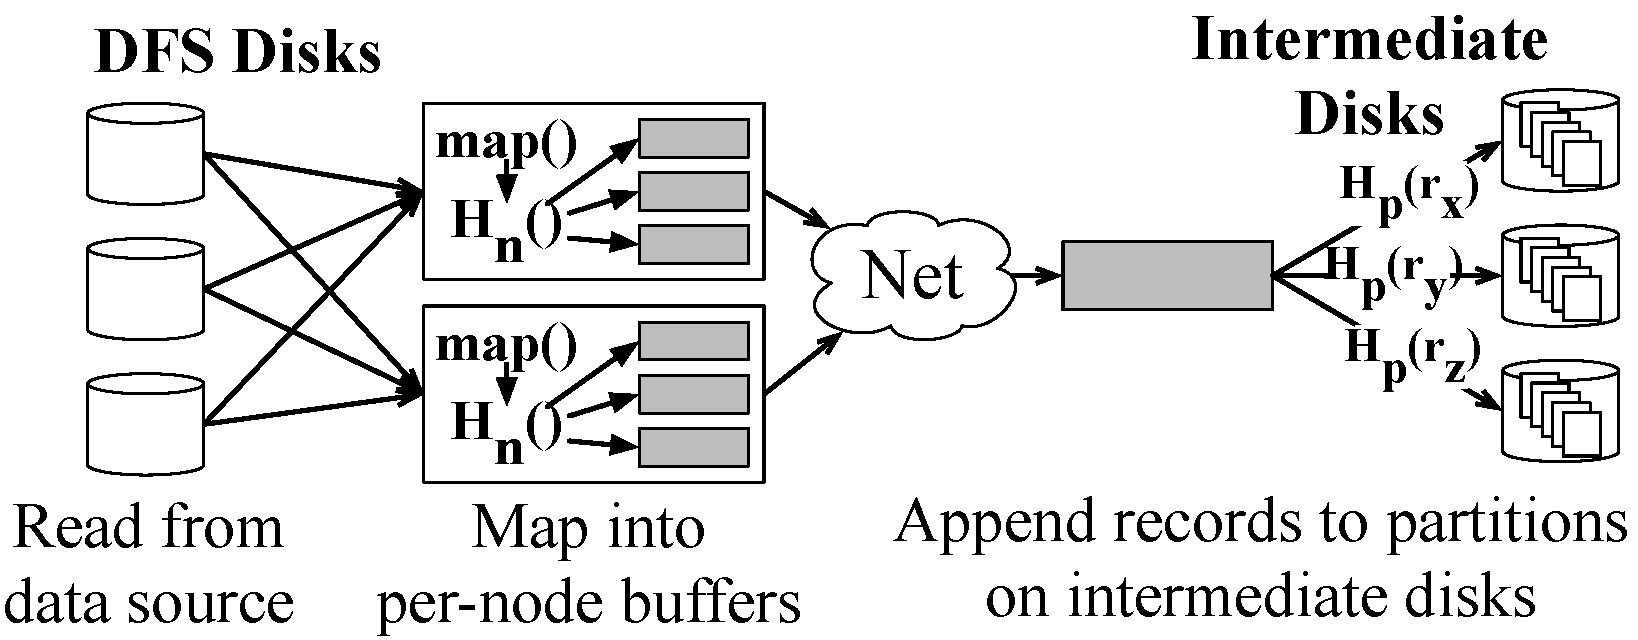
\includegraphics[width=\columnwidth]{fault_tolerance/figures/detailed_phase_one.pdf}
  \caption{\label{fig:phase_one} Phase One}
  \end{subfigure}\vspace{1em}
  \begin{subfigure}[t]{\columnwidth}
  \centering
  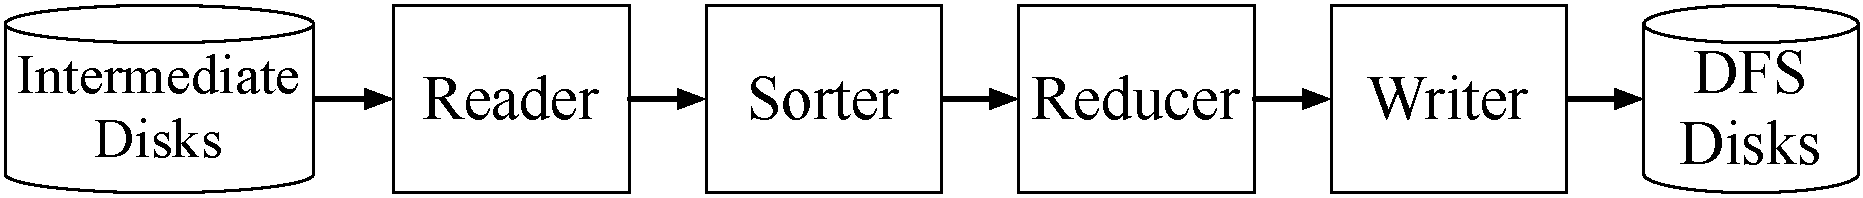
\includegraphics[width=\columnwidth]{fault_tolerance/figures/phase_two.pdf}
  \caption{\label{fig:phase_two} Phase Two}
  \end{subfigure}

  \caption{\label{fig:themis_phases} A diagrammatic overview of \themis' phases.}
\end{figure}

Nodes in a \themis cluster each have a collection of \emph{intermediate disks}
that store volatile intermediate data and a disjoint collection of \emph{DFS
  disks} that store input and output data, and are typically under the control
of a distributed file system like HDFS.

\themis runs a MapReduce job in two main \emph{phases}, called \emph{phase one}
and \emph{phase two}.  In phase one, input records are read in parallel from
the cluster's DFS disks. \themis applies the \map function to each record,
producing a collection of \emph{intermediate records} that are written to
intermediate partitions spread across the cluster's intermediate disks. Each
intermediate partition holds all records with a certain set of keys. The
mapping from keys to intermediate partitions is determined by a \emph{partition
  function}. Phase one is roughly analogous to Hadoop's map and shuffle phases.

At the end of phase one, all intermediate records have been generated,
partitioned and stored across the cluster's intermediate disks. A diagrammatic
overview of phase one is given in Figure~\ref{fig:phase_one}.

In phase two, each intermediate partition is read from the cluster's
intermediate disks completely into memory. Once in memory, it is sorted in-core
by key, and the \reduce function is applied to each group of records in the
partition with the same key. This produces a collection of \emph{output
  records} that are written to files on the DFS disks. Phase two is roughly
equivalent to Hadoop's sort and reduce phases. A diagrammatic overview of phase
two is given in Figure~\ref{fig:phase_two}.

Note that phase one requires all-to-all communication among cluster nodes, but
that phase two can be executed on each node independently.

\subsubsection{Partitioning}

In order for phase two to be processed efficiently, partitions should be small
enough for several of them to be processed in memory
simultaneously. Additionally, they should be as uniformly-sized as possible to
prevent stragglers. The partition function is responsible for ensuring both
these properties. The user can provide their own partition function, or it can
be derived at runtime through an optional sampling phase called \emph{phase
  zero}. Phase zero requires a fairly small sample to produce a good partition
function, and typically takes under a minute to run.


\subsection{Recovery Mechanism}
\label{sec:recovery}

As described in Section~\ref{fault_tolerance:sec:design}, recovering from a
failure consists of two central actions: write recovery and read recovery. In
the case of \themis, write recovery involves recovering partitions on any
intermediate disk that failed, while read recovery involves re-generating
missing pieces of partitions that a failed node should have produced, but
didn't. When a job fails, \themis will recover it by running a \emph{recovery
  job}, which is treated like a normal MapReduce job but is dedicated to
recovery.

\begin{figure}
  \centering
  \begin{subfigure}[t]{\columnwidth}
    \centering
    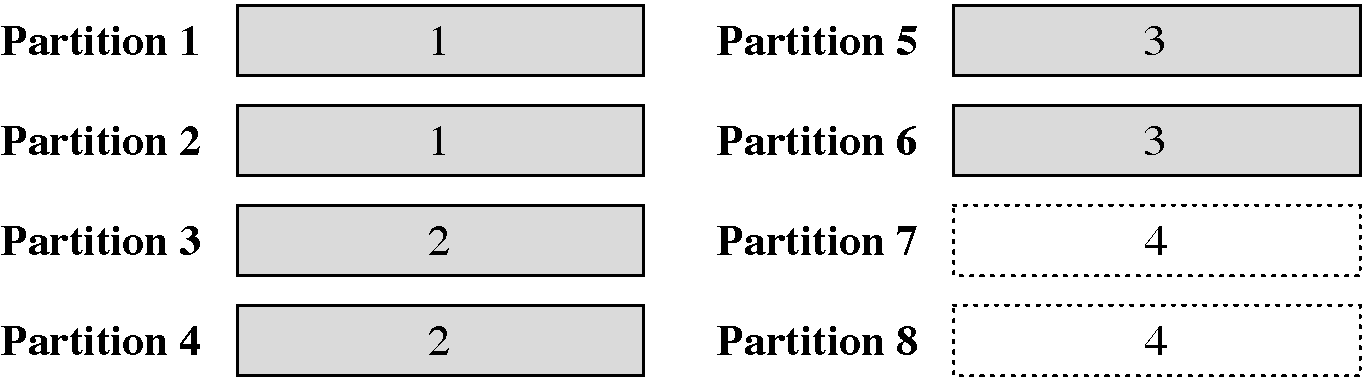
\includegraphics[width=\textwidth]{fault_tolerance/figures/disk_failure_before_recovery}
    \caption{\label{fig:disk_fail_before} The state of the job's intermediate
      partitions after the failure of disk 4. All intermediate partitions
      stored on disk 4 has been lost.}
  \end{subfigure}\hspace{0.05\textwidth}
  \begin{subfigure}[t]{\columnwidth}
    \centering
    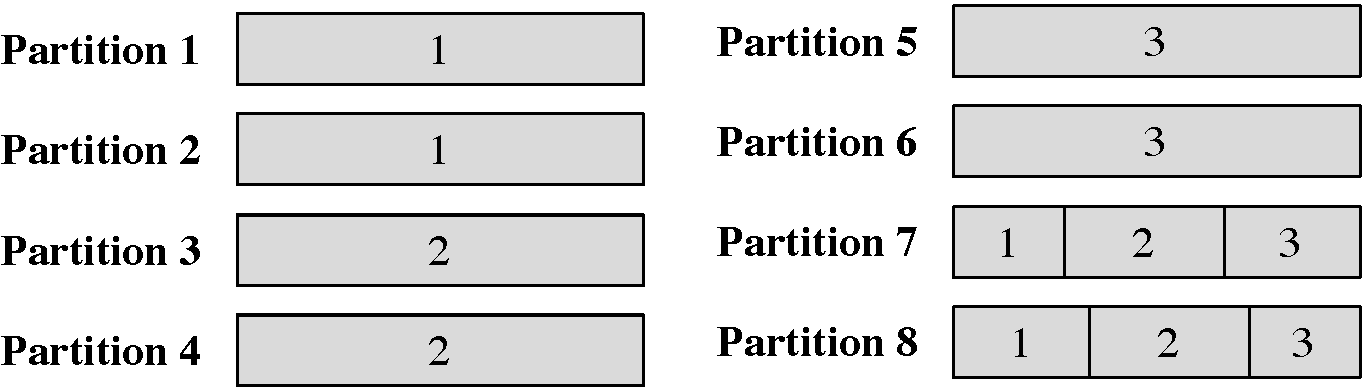
\includegraphics[width=\textwidth]{fault_tolerance/figures/disk_failure_after_recovery}
    \caption{\label{fig:disk_fail_after} The state of the job's intermediate
      partitions after recovery from the disk failure. Intermediate data for
      the partitions on disk 4 have spread across disks 1 through 3.}
  \end{subfigure}
  \caption{\label{fig:disk_fail} Illustrative example of disk failure and
    recovery in a two-node cluster with two intermediate disks per node and
    eight intermediate partitions. The rectangles
    representing each partition are labeled with the disk or disks on which
    data for that partition is stored.}
\end{figure}

Before we explore the technical details of the implementation, consider the
following illustrative example. Suppose that \themis is running on a two-node
cluster with two intermediate disks each, storing a total of eight intermediate
partitions for a particular job. In Figure~\ref{fig:disk_fail_before}, disk 4
in this cluster has failed during phase one, causing the loss of partitions 7
and 8. Figure~\ref{fig:disk_fail_after} shows the state of the intermediate
partitions at the end of phase one of the recovery job, when the data for
partitions 7 and 8 has been recovered.

Note that the recovered data for partitions 7 and 8 is spread across all the
remaining disks roughly evenly; this is highly desirable because it allows as
many disks as possible to participate in phase two of the recovery job. It
should also be noted that after the failure of disk 4 in phase one, phase two
can be run to completion on partitions 1 through 6 without waiting for the
recovery job to recover the other partitions.

\begin{figure}[t]
  \centering
  \begin{subfigure}[t]{\columnwidth}
    \centering
    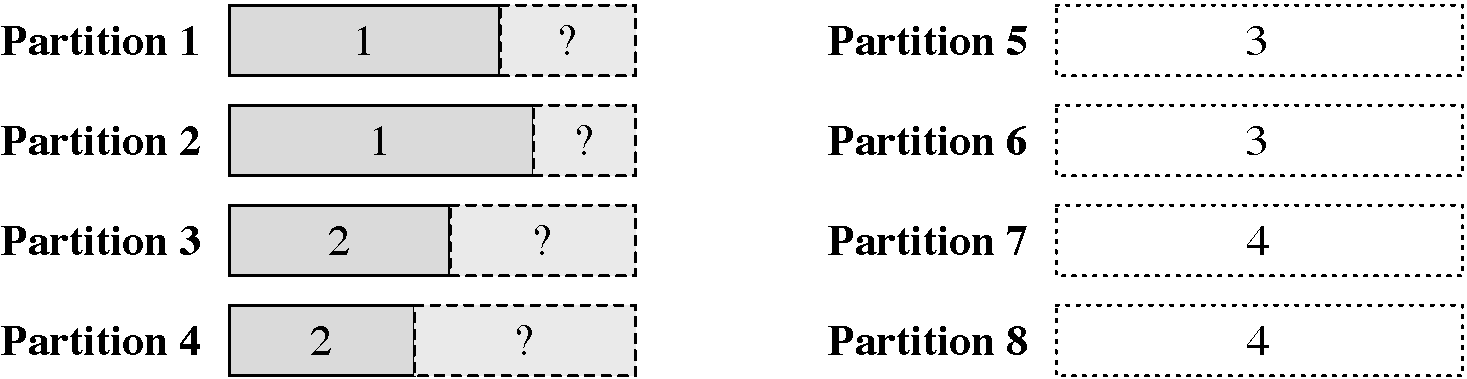
\includegraphics[width=\textwidth]{fault_tolerance/figures/node_failure_before_recovery}
    \caption{\label{fig:node_fail_before} The state of the job's intermediate
      partitions after the failure of node 2. All intermediate data for disks 3
      and 4 has been lost, and some data for the remaining partitions may not
      have been generated.}
  \end{subfigure}\hspace{0.05\textwidth}
  \begin{subfigure}[t]{\columnwidth}
    \centering
    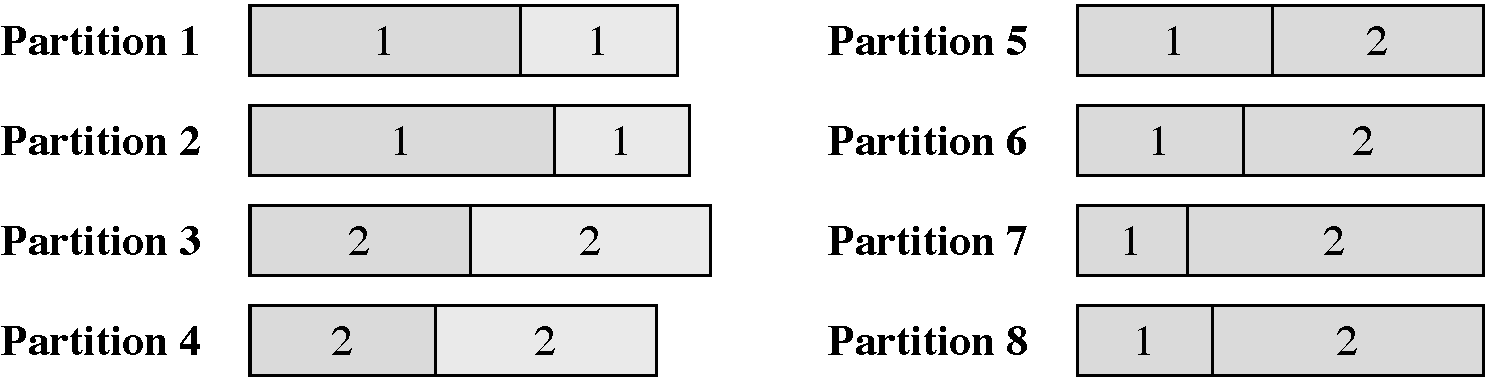
\includegraphics[width=\textwidth]{fault_tolerance/figures/node_failure_after_recovery}
    \caption{\label{fig:node_fail_after} The state of the job's intermediate
      partitions after recovery from the node failure. Intermediate data for
      the partitions on disks 3 and 4 have spread across disks 1 and 2, and
      data that should have been produced by node 2 has been added to node 1's
      partitions (although there may be duplicates).}
  \end{subfigure}
  \caption{\label{fig:node_fail} Illustrative example of node failure and
    recovery in a two-node cluster with two intermediate disks per node and
    eight intermediate partitions. A '?' indicates that it is unknown
    whether the data has been lost or not.}
\end{figure}

Figure~\ref{fig:node_fail_before} shows the same cluster after experiencing a
failure of an entire node. Not only have partitions 5 through 8 been lost, but
the remaining partitions are incomplete because the node did not finish
producing intermediate data for those partitions before it failed. Once phase
one of the recovery job has completed in Figure~\ref{fig:node_fail_after},
write recovery has spread the lost data from partitions 5 through 8 across
disks 1 and 2, while read recovery has ensured that every record that belongs
in partitions 1 through 4 has been written at least once.

\begin{table*}[t]
  \centering
  \caption{\label{table:failure_response} Table summarizing \themis' response
    to various kinds of failures at different points in the job.}
  \resizebox{\columnwidth}{!}{
  \begin{tabular}{|c|c|c|c|c|}
    \hline
    \textbf{Phase} & \textbf{Failure} & \textbf{Write Recovery} & \textbf{Read Recovery} & \textbf{Run Subsequent Phases?} \\
    \hline
    Zero (Sample) & Any & None & None & Yes \\
    One (Map + Shuffle) & Disk & Failed disk's partitions & None & Yes \\
    One (Map + Shuffle) & Node & All node's disks' partitions & Node's input files & No \\
    Two (Sort + Reduce) & Disk & Failed disk's partitions & None & Yes \\
    Two (Sort + Reduce) & Node & All node's disks' partitions & None & Yes \\
    \hline
  \end{tabular}
}
\end{table*}

In contrast to disk failure, phase two cannot be run after a node failure in
phase one because some intermediate partitions may not be complete.

If a disk or node fails in phase two, write recovery must be performed to
restore the intermediate data that was lost in the failure, but no read
recovery must be performed. Since phase zero is optional and does not produce
any output aside from a partition function, any failure during phase zero
simply requires re-executing it.

The responses to various kinds of failure in each of \themis' stages is
summarized in Table~\ref{table:failure_response}.

In the following sections, we will describe the mechanisms behind both write
and read recovery.

\subsubsection{Write Recovery}

To perform write recovery, the recovery job must re-map the failed job's input,
discarding any records that were not stored on the intermediate disks that
failed. To do this, the recovery job wraps its partition function in a
\emph{record filter}. This filter is applied to each record before it is passed
to the partition function. Abstractly, a record filter is a function that takes
a record as input and returns either ``accept'' or ``reject''. The filter
accepts a record if the record belongs to one of the partitions being
recovered, and rejects it otherwise.

In practice, \themis accomplishes record filtering in one of two ways. If the
failed job was using a user-defined partition function, the record filter
applies the failed job's partition function to the record. If the resulting
partition number is outside the range of partitions to be recovered, the filter
rejects the record.

If the original job is using a partition function generated by phase zero, the
record filter stores a set of boundary key ranges, one per contiguous range of
partitions being recovered. The complete list of boundary keys for each
partition is stored on distributed storage at the end of phase zero, and the
filter retrieves the appropriate boundary keys when it is constructed.

When an intermediate record is emitted by the \map function, the filter first
compares each intermediate record's key to the boundaries of each of its
ranges; if the record is within any of the filter's ranges, the filter
accepts the record.

In order to speed recovery by writing to as many disks in parallel as possible,
the intermediate data being recovered is spread across the cluster's remaining
intermediate disks. This is done by running phase zero during the recovery job
on a filtered sample of the input data, which generates a partition function
that spreads data in the filtered partition ranges evenly throughout the cluster.

At the end of phase one of the recovery job, any partitions that were
completely lost during a failure have been reconstituted and spread across the
cluster's remaining intermediate disks.

\subsubsection{Read Recovery}

As Table~\ref{table:failure_response} illustrates, read recovery is always
performed alongside write recovery. We take advantage of this by piggybacking
read recovery on write recovery.

In order to perform read recovery, we must first know the set of files that
were not completely processed by the failed node. \themis tracks which files
were completely mapped and received using a form of end-to-end
acknowledgments~\cite{endtoendargument}.  When a node is done reading a file in
phase one, it sends an EOF, or ``end-of-file'', annotation to every node in the
cluster indicating that the node will not receive any more data for the
file. Special care is taken to ensure that every intermediate record associated
with the file is transferred before this annotation. When a node receives an
EOF annotation, it adds the file's file ID to a list. At the end of phase one,
these lists are merged together to form a list of the nodes that received each
file. If every live node received an EOF annotation for a file, performing read
recovery on that file is not necessary. Each input file is checked for this
condition when constructing the input file list for a recovery job and files
are flagged for read recovery as appropriate.

Once phase one has completed, two sets of intermediate files will exist for the
failed job: the partially-complete set of files from the failed job and the set
of files generated as a result of read recovery. It is likely that some of the
records in these files are duplicates, and any duplicate records must be
removed to retain the \reduce function's correctness. To distinguish
intermediate records from one another, \themis tags each intermediate record
with \emph{source metadata} that uniquely identifies the record.

To uniquely identify intermediate records, we leverage the common assumption
that the \map function is deterministic and, as such, that applying the \map
function to an input record creates a totally-ordered sequence of intermediate
records. We identify an intermediate record by the position of its ``parent''
input record within the input dataset and its position in the totally-ordered
sequence of intermediate records. Specifically, we tag each record with a
64-bit file GUID, a 64-bit offset, and a 32-bit intermediate record ID. For the
purposes of evaluation, we store all 20 bytes of metadata even if the metadata
could potentially be compressed; note that for records with small offsets and
intermediate record IDs, these three pieces of metadata require far less than
20 bytes per record to store.

In phase two, intermediate partitions from the failed and recovery jobs with
the same intermediate partition number are concatenated together into an
in-memory buffer and sorted as a single intermediate partition. Before the
\reduce function is called on a set of intermediate records with a given key,
that set of records is secondarily sorted by its source metadata. The \reduce
function's record iterator then skips any records whose source metadata is the
same as that of the previous record.


\subsection{Multi-Tenancy in \themis}
\label{sec:multi-tenancy}

Each \themis node runs as a single process that assumes that it has exclusive
access to its intermediate disks and that it will not experience
memory pressure from other processes that results in swapping as long as it
does not exceed its configured memory limit. Its memory and disk management
subsystems (described in detail in~\cite{themis} and~\cite{tritonsort}) rely on
these assumptions and are the key enablers of \themis' I/O-efficiency and high
performance. Hence, running multiple \themis processes on a single node would
result in degraded performance since the processes would interfere with one
another.

\begin{figure}
  \centering
  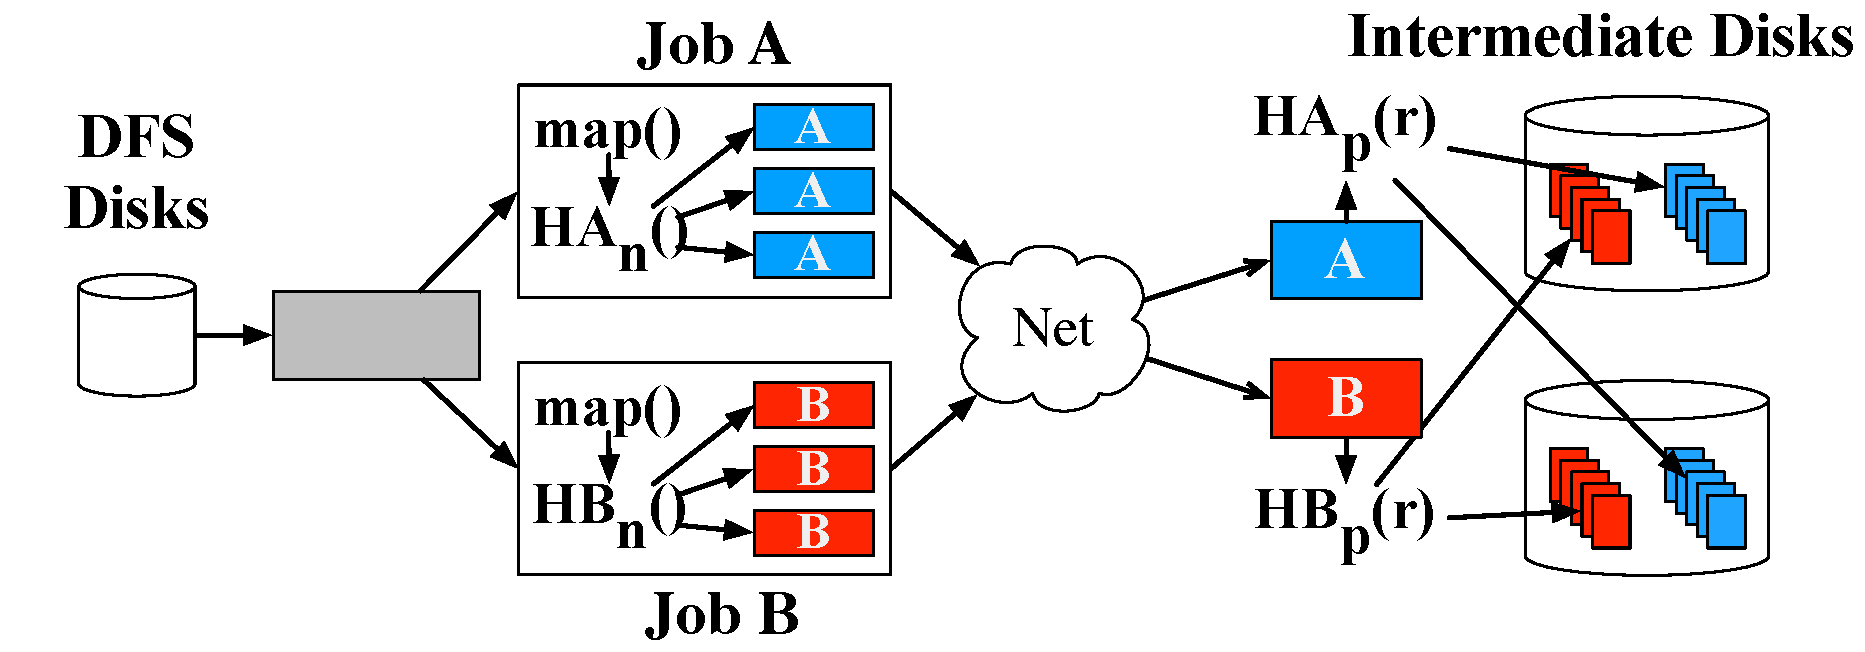
\includegraphics[width=\columnwidth]{fault_tolerance/figures/multi_tenancy}
  \caption{\label{fig:multi_tenancy} An overview of multi-tenancy in
\themis. Input records are mapped by both job A and job B's \map functions,
and intermediate records are routed based on each job's partition function independently.}
\end{figure}

To allow multiple jobs to run simultaneously in \themis with minimal
interference, we have modified \themis to support running multiple jobs
concurrently within a single process. To allow for this concurrent processing,
records read from disk are passed through each job's \map function one function
at a time, but intermediate records are transferred and written in
parallel. Buffers of intermediate records produced by a \map function are
tagged with the unique ID of that \map function's job before being sent to the
appropriate destination node. Once a buffer is received, this job ID is used to
determine to which set of intermediate partitions the buffer's records will be
written. This process is illustrated in Figure~\ref{fig:multi_tenancy}

A unique feature of our deployment prototype is that it does not co-schedule
\map and \reduce function computation. Instead, it organizes jobs into
\emph{batches}, and runs phases one and two for all jobs in a batch
simultaneously before processing the next batch. If phase zero needs to be run
to compute partition functions for any of these jobs, it is run on each job in
the batch individually before phase one starts.


\subsection{Job Dispatch}
\label{sec:control_plane}

The execution of batches of jobs is controlled by a \emph{cluster
  coordinator}. The cluster coordinator accepts descriptions of batches from
clients and coordinates their execution across the cluster's machines. Each
machine in the cluster runs a \emph{node coordinator} that is responsible for
running a \themis process on its machine and reporting an error if it crashes.

Messages are exchanged between the user, the cluster coordinator and the node
coordinators through the manipulation of message queues. Additionally, the
coordinators maintain metadata about both themselves and the jobs they run. In
our current implementation, the role of message queues and metadata store are
both filled by a Redis~\cite{redis} database. Redis was chosen primarily for
convenience; a scalable key-value store like Hyperdex~\cite{hyperdex} or
Cassandra~\cite{cassandra} and message queue like Kafka~\cite{kafka} or
Kestrel~\cite{kestrel} could be substituted.

To run a batch, the user pushes a description of the jobs in the batch to the
cluster coordinator's job queue. Upon dequeuing a batch, the cluster
coordinator assigns a unique job ID to each job in the batch. It then determines
the set of input files that each job will process, and divvies those files out
among nodes. We describe this process in more detail in
Section~\ref{sec:input_file_gathering}.


\subsection{Input Files and Distributed Storage}
\label{sec:input_file_gathering}

\begin{figure}
  \centering
  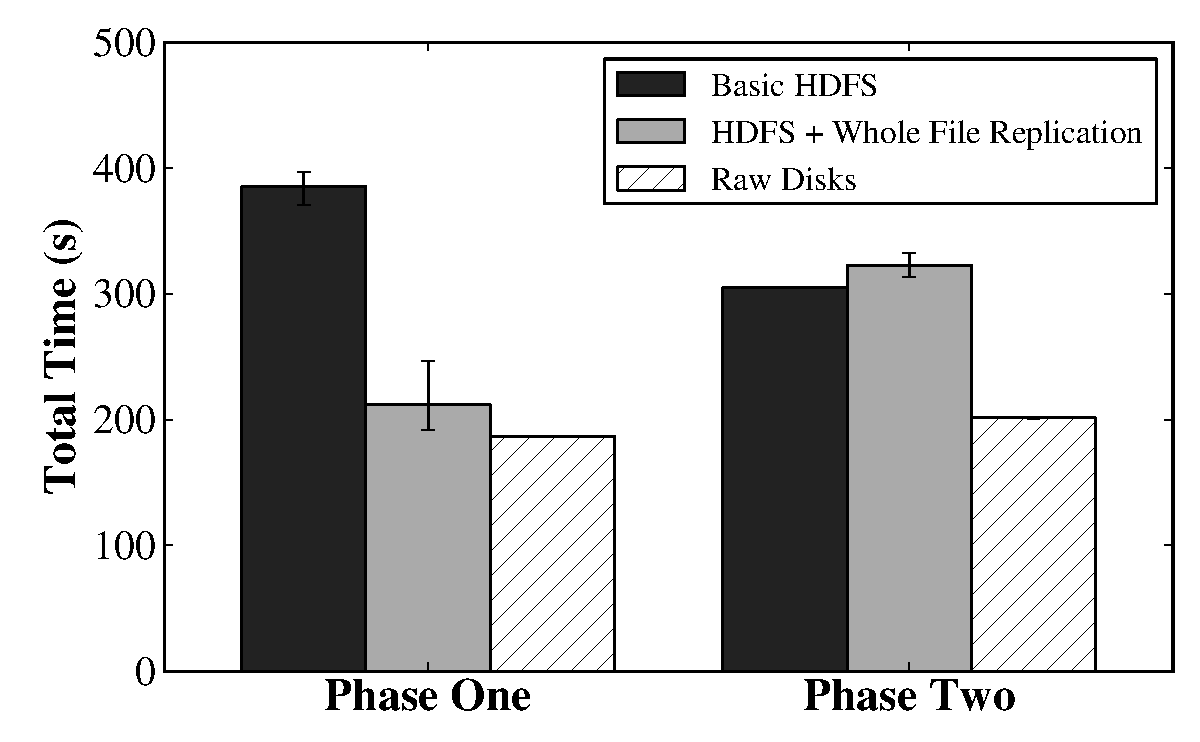
\includegraphics[width=\columnwidth]{fault_tolerance/graphs/hdfs_no_proxy_penalty}
  \caption{\label{fig:hdfs_no_proxy_penalty} Comparing the performance of
    unmodified HDFS, HDFS with whole file replication for the primary replica,
    and reading and writing from raw disks.}
\end{figure}

The specification of each \themis job includes an input directory; all files in
the input directory are processed. \themis can read input files from raw disks
or from HDFS~\cite{hdfs} using the WebHDFS REST API. We use HDFS exclusively in
this work.

Each file is uniquely identified by its URL, which is of the form\\
\texttt{<protocol>://<host>:<port>/<path from root>}. Each file is also given a
file ID that must be unique within the job. In our implementation, a
file's ID is the upper 64 bits of the MD5 hash of its URL.

Our main concern when moving from raw disks to distributed storage was
maximizing the amount of bandwidth we could achieve from the storage system.
In order to achieve sufficient bandwidth, we found that we needed to change the
way HDFS allocates blocks for files. In particular, we modified HDFS so that it
performs \emph{whole-file replication} of the file's primary replica by placing
every block on a specific disk in the cluster based on the file's name. For
example, a file named \texttt{/1.2.3.4/3/<path>} would be stored on the third
DFS disk on node \texttt{1.2.3.4}. To allow \themis to remain oblivious to this
scheme, we implemented a proxy that performs a basic round-robin allocation of
primary file replicas to cluster disks and transparently maps between regular
and placement-aware paths. The proxy only interposes itself in communication
between \themis and HDFS when a file is first opened, and imposes no additional
overhead thereafter.

Figure~\ref{fig:hdfs_no_proxy_penalty} compares the performance of an 800GB, 8
node sort with and without these modifications; as a reminder, phase one of
\themis reads sequentially from HDFS, while phase two writes sequentially to
it. The substantial performance improvement for reads is the result of the
elimination of read contention on each node's DFS disks when many files are
being read simultaneously. However, the increased rigidity of block allocation
imposed by the proxy makes the performance of writes slightly worse than
unmodified HDFS.

We found that HDFS' block placement APIs were not sufficient for providing
whole-file replication for all of a file's replicas. Hence, blocks for all
other replicas are allocated according to HDFS' default policy, and access to
non-primary replicas occurs at the speed of unmodified HDFS. The cluster
coordinator will assign files to nodes that contain their primary replica
whenever possible.


\subsection{Responding to Failures}
\label{sec:fault_response}

As node coordinators run, they refresh a keep-alive key in Redis every few
seconds; if a node fails to refresh its keep-alive key, the cluster coordinator
presumes that the node has failed. A node notifies the cluster coordinator
directly if it finds that it can no longer write to one of its intermediate
disks.

\themis attempts to insulate the rest of the cluster from a failure whenever
one occurs so that the healthy portion of the cluster can complete as much work
as possible. To avoid the attendant complexity and fragility of coordinating
failure notification across nodes, \themis simply discards any data meant for a
failed portion of the cluster. When a node fails, all existing TCP sockets to
that node will break. Nodes respond to broken sockets by discarding all data
meant for that socket for the remainder of the batch. Similarly, when a disk
fails, all data that would have been written to the failed disk for the rest of
the batch is discarded. Subsequent batches will not use failed disks or nodes
until an operator has explicitly marked them as having recovered.

Currently, the user is responsible for issuing a recovery job to recover a
failed job. Scheduling recovery jobs to maximize the likelihood of scan sharing
is beyond the scope of this work; we examine some related efforts relevant to
this problem in Chapter~\ref{chapter:related_work}.


\section{Per-Record Replay Proportionality}
\label{sec:recovery_cost}

\begin{figure}
  \centering
  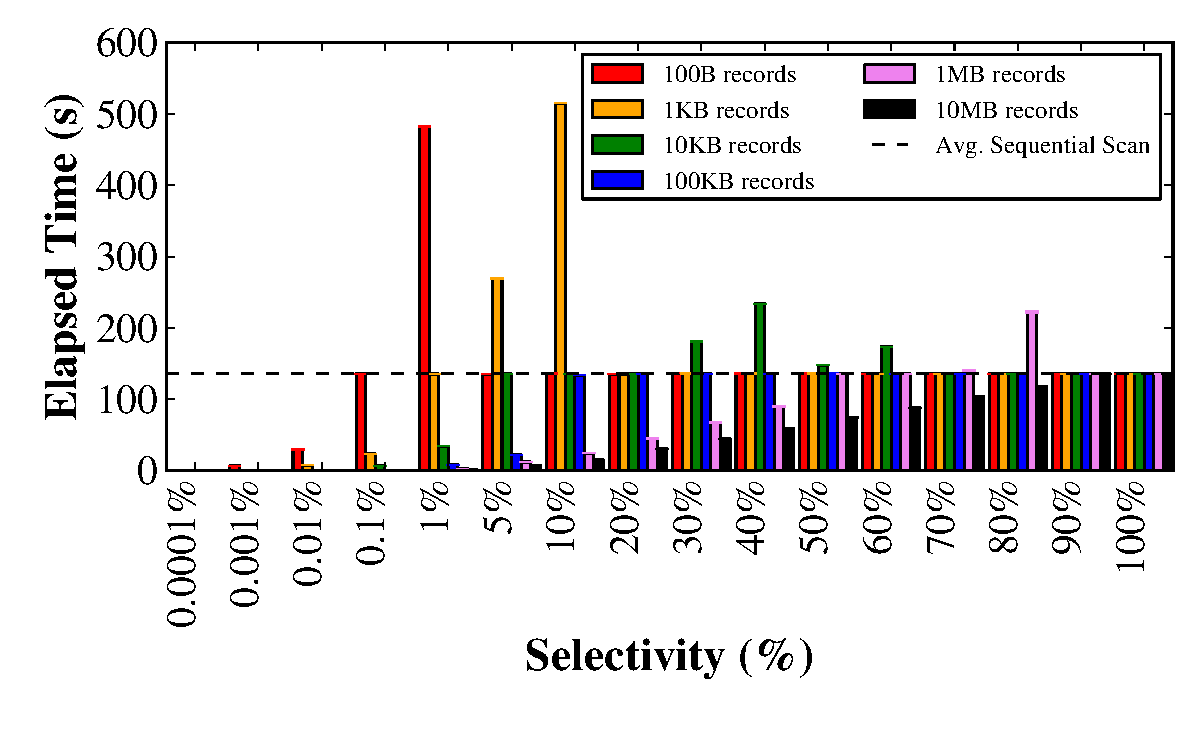
\includegraphics[width=\columnwidth]{fault_tolerance/graphs/scan_vs_seek}
  \caption{\label{fig:seek-vs-scan} Time to sequentially scan a 13.5 GB file
    vs. selectively reading a percentage of records.}
\end{figure}

\begin{figure*}
  \centering
  \begin{subfigure}[b]{\textwidth}
    \centering
    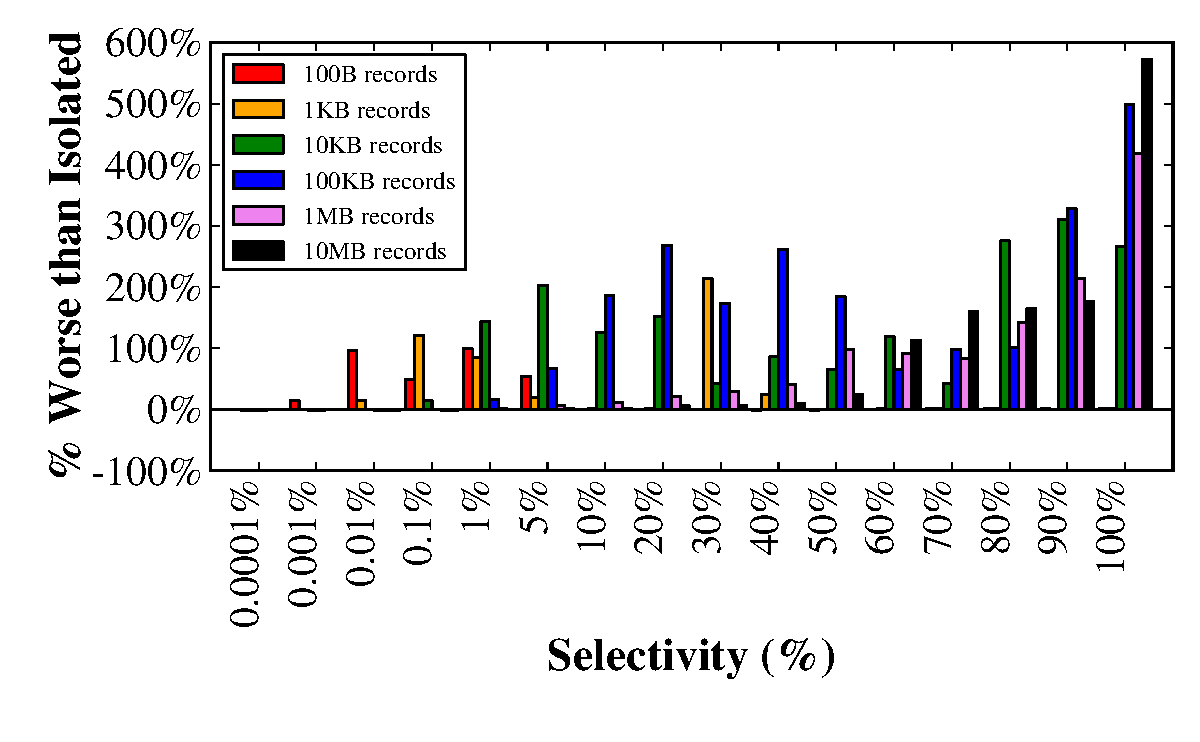
\includegraphics[width=\textwidth]{fault_tolerance/graphs/simultaneous_scan_same_file}
    \caption{\label{fig:simultaneous_same_file_scan} The effect of
      simultaneity on sequential scans.}
  \end{subfigure}
  \begin{subfigure}[b]{\textwidth}
    \centering
    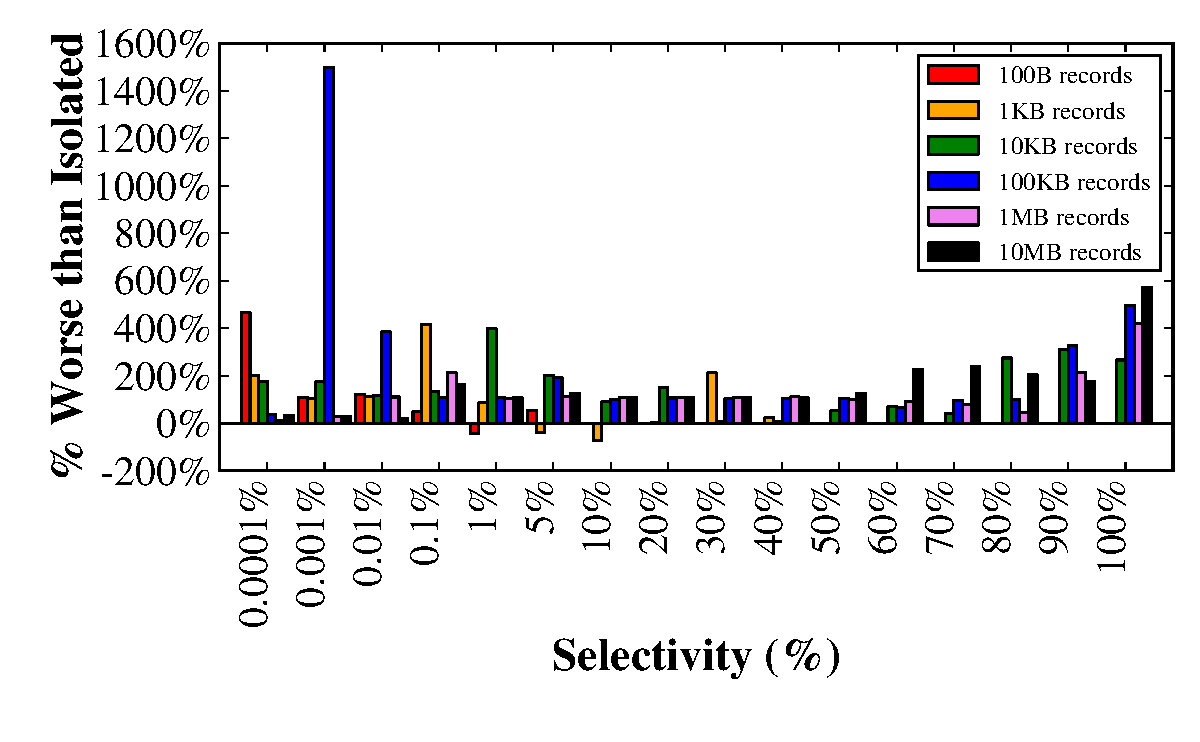
\includegraphics[width=\textwidth]{fault_tolerance/graphs/simultaneous_seek_same_file}
    \caption{\label{fig:simultaneous_same_file_seek} The effect of
      simultaneity on selective reads.}
  \end{subfigure}
  \caption{\label{fig:simultaneous_same_file} The negative impact of
    both scanning through and selectively reading from the same file simultaneously.}
\end{figure*}

\begin{figure*}
  \centering
  \begin{subfigure}[b]{\textwidth}
    \centering
    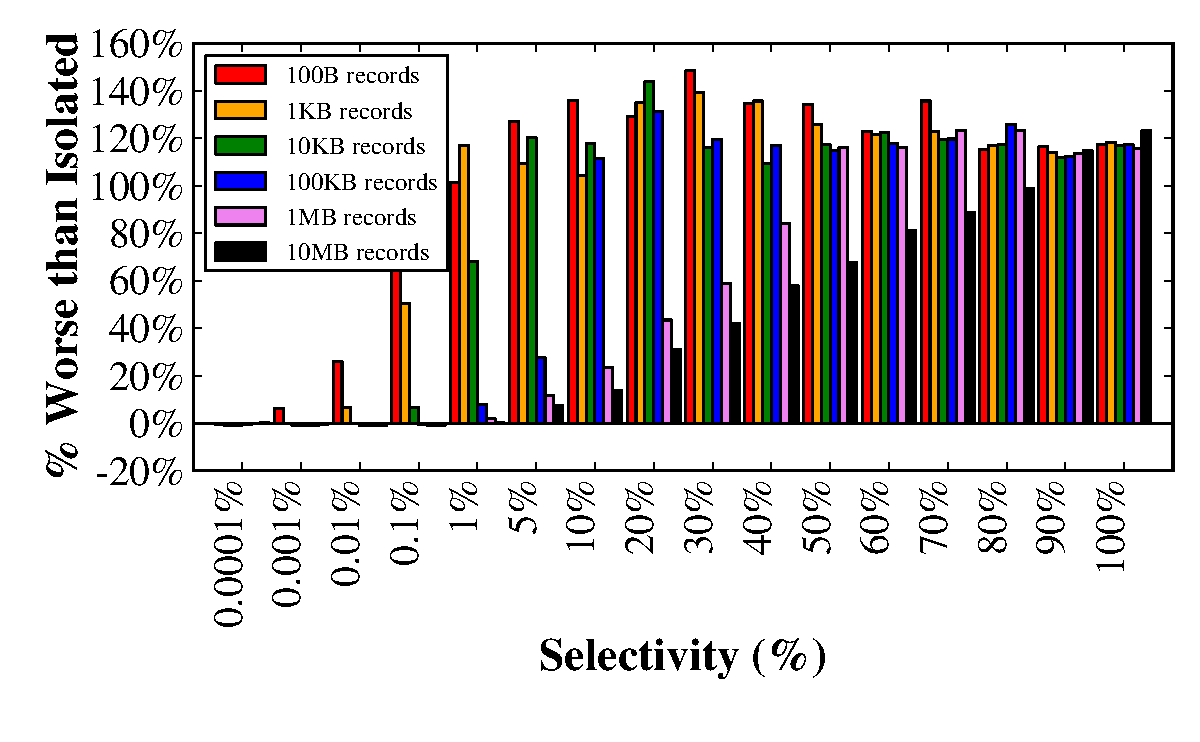
\includegraphics[width=\textwidth]{fault_tolerance/graphs/simultaneous_scan_different_files}
    \caption{\label{fig:simultaneous_different_files_scan} The effect of
      simultaneity on sequential scans.}
  \end{subfigure}
  \begin{subfigure}[b]{\textwidth}
    \centering
    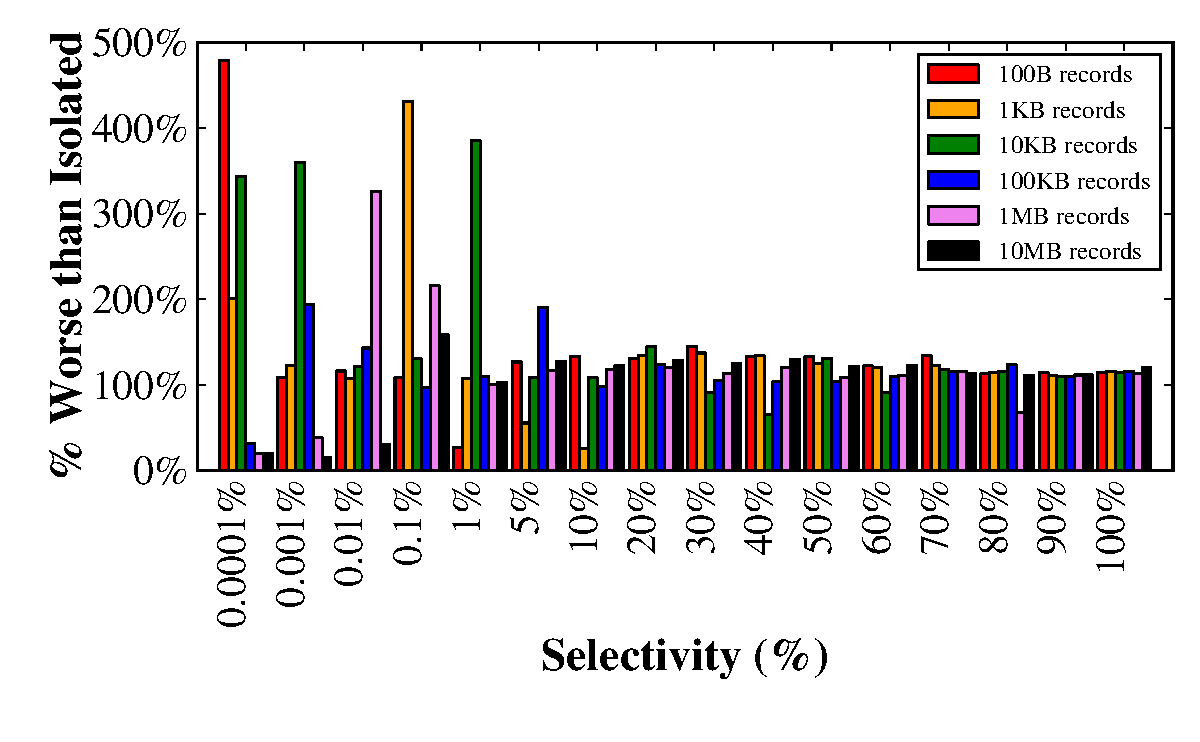
\includegraphics[width=\textwidth]{fault_tolerance/graphs/simultaneous_seek_different_files}
    \caption{\label{fig:simultaneous_different_files_seek} The effect of
      simultaneity on selective reads.}
  \end{subfigure}
  \caption{\label{fig:simultaneous_different_files} The negative impact of
    running a scan on one file while selectively reading records from a
    second file.}
\end{figure*}

When examining our options for adding fault tolerance to \themis, we were
particularly motivated by the idea of being able to recover by only reading and
re-mapping records whose intermediate data contributed to failed intermediate
partitions. We recognized that the overhead of storing this information would
potentially be quite high; in general, it requires storing information about
the lineage and intermediate partition of every intermediate
record. Nonetheless, we wanted to gain an understanding of the regimes in which
this overhead might be a reasonable tradeoff for a decreased recovery time. In
this section, we examine the potential benefits and disadvantages of this
approach using a microbenchmark.

To evaluate the potential time savings from selectively reading the subset of
input records needed to perform recovery, we created a 13.5 GB file on one of
our cluster's disks and compared the time taken to completely scan through the
file with the time taken to read a certain percentage of the file's
records. The percentage of records selectively read roughly corresponds to the
``selectivity'' of the recovery being simulated. For example, if 1\% of records
are being read, this corresponds to the amount of reading necessary to recover
from a lost of 1\% of the cluster's intermediate partitions.

As a simplifying assumption, we assumed that the records are evenly spaced
throughout the file. We completely purged the operating system's file buffer
cache and disabled any caching on our disk controllers so that each experiment
started from a cold cache.

As Figure~\ref{fig:seek-vs-scan} shows, when the selectivity of recovery is
quite small, selective reads can achieve large speedups over a sequential
scan. However, selectively reading records is far from proportional. For
example, for a file with 1KB records, the cost of sequentially scanning the
file is the same as the cost of selectively reading 1\% of its records; this
means that the loss of more than 1\% of the cluster's intermediate partitions
can be recovered from just as quickly by scanning input files as it can by
selectively reading them for I/O-bound jobs.

We suspect that this non-proportionality is due to a combination of the
overhead of seeking between records, the overhead of the relatively many
\texttt{read()} syscalls needed to retrieve those records, and the behavior of
the operating system's buffer cache. Note that for certain record sizes and
selectivities, selective reading performs dramatically worse than sequential
scanning; this is due mainly to poor interaction between the application and
the buffer cache.

In addition to its non-proportionality, selective reads have a negative impact
on the performance of other concurrent operations to the same
disk. Figure~\ref{fig:simultaneous_same_file} shows that selectively reading
from a file while scanning through it simultaneously can decrease the speed of
the scan by up to 600\%. We believe that cache interference between the two
writing processes, as well as the mechanical act of disrupting the sequentiality
of disk access with seeking, are the source of these overheads.

Figure~\ref{fig:simultaneous_different_files} shows the impact of running a
scan and a selective read over two different files on the same disk
simultaneously. Here the performance decrease for scans is much less drastic;
we believe the primary source of this performance decrease to be the overhead
imposed on the scan by disk seeks.

These results indicate, somewhat intuitively, that when the selectivity of the
recovery is very small (less than 0.01\%), it is highly beneficial to perform
selective reads. However, selective reads are only a proportional form of fault
tolerance if records are relatively large, and they have the potential to
interact poorly with other concurrent sequential scans. In addition, a recovery
with small selectivity is only likely when the cluster is fairly large, which
is a different operating environment from the ``dense'' clusters on which we
focus in this work.

\section{Evaluation}
\label{fault_tolerance:sec:eval}

In Section~\ref{fault_tolerance:sec:methodology}, we describe our experimental methodology. In
Section~\ref{sec:proportionality}, we show that recovery from both disk and
node failure are proportional, in that the time taken to recover is
proportional to the size of the failure. In
Section~\ref{sec:scan_sharing_overhead}, we show that the overhead imposed by
scan sharing a normal job with a recovery job is low.

\subsection{Methodology}
\label{fault_tolerance:sec:methodology}

We evaluated our fault tolerance mechanisms on eight of the machines in the
cluster described in Section~\ref{sec:hardware_architecture}. Each hard drive
is configured with a single XFS partition that is configured with a single
allocation group to avoid file fragmentation across allocations groups and is
mounted with the \texttt{noatime}, \texttt{nobarrier} and \texttt{noquota}
flags set. For this evaluation, all servers were running Linux 2.6.32. Jobs
source and sink data to HDFS, configured with 128MB blocks and whole-file
replication of the primary replica of each file.

\themis is written in C++ and, in this evaluation, is compiled with
\texttt{g++} 4.7.1. The cluster coordinator, node coordinator and HDFS
rewriting proxy are written in Python.

We rely on the sort MapReduce job to evaluate our fault tolerance
mechanisms. Since sort corresponds to no-op \map and \reduce functions, it
provides a natural way of evaluating fault tolerance independently of the job
being performed. At the same time, sort's large intermediate data set size
allowed us to stress-test the system's ability to scale
proportionally. Additionally, we have found it logistically difficult to both
obtain and store freely-available data sets that are sufficiently large that
they do not fit in a single node's memory. The input data set for sort is easy
to generate synthetically, which allows us to scale the evaluation beyond a
single node.

\subsection{Proportionality of Recovery}
\label{sec:proportionality}

In this section, we explore the proportionality of our recovery process in
response to disk and node failures.

\subsubsection{Recovering From Disk Failure}
\label{sec:disk_proportionality}

\begin{figure}
  \centering
  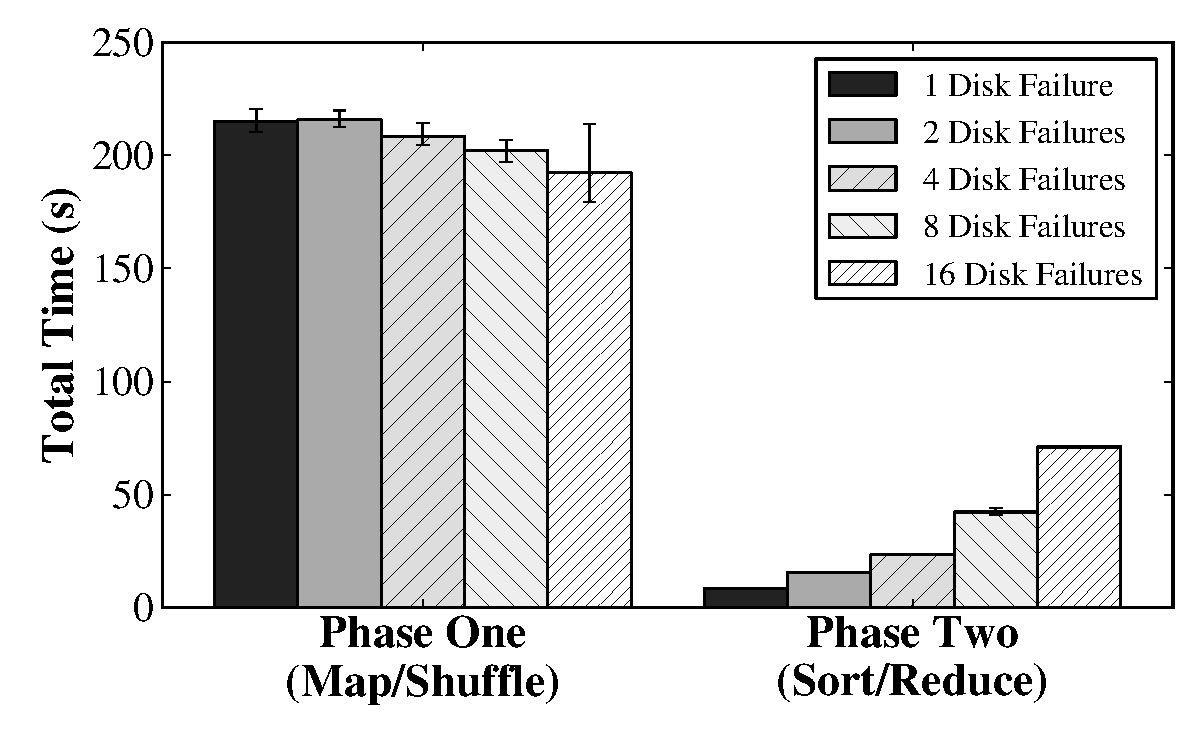
\includegraphics[width=\columnwidth]{fault_tolerance/graphs/disk_recovery_proportionality.pdf}
  \caption{\label{fig:disk_recovery_proportionality} Runtime of recovery from a
    disk failure during an 800GB sort with an increasing number of failed
    disks.}
\end{figure}

To test the proportionality of recovery from a disk failure, we ran an 800GB
sort job across our eight-node testbed and failed an increasing number of disks
during phase one. Disk failures were injected into the system by making the
part of \themis that writes to intermediate disks fail after it had written a
certain number of bytes to the disks we wanted to fail. We then ran a recovery
job to recover the data from those failed
disks. Figure~\ref{fig:disk_recovery_proportionality} shows the elapsed time of
both phases for the recovery job.

The elapsed time of the recovery job's phase two increases sub-linearly as the
number of disk failures increases.  This is because phase two is designed to
process multiple intermediate partitions in parallel and the number of
partitions created during recovery is fairly small, so processing twice as many
partitions doesn't necessarily take twice as much time. The decrease in phase
one's recovery time as the number of disks to recover increases is coincidental
and simply reflects the variability of access time provided by HDFS.

\subsubsection{Recovering From Node Failure}

\begin{figure}
  \centering
  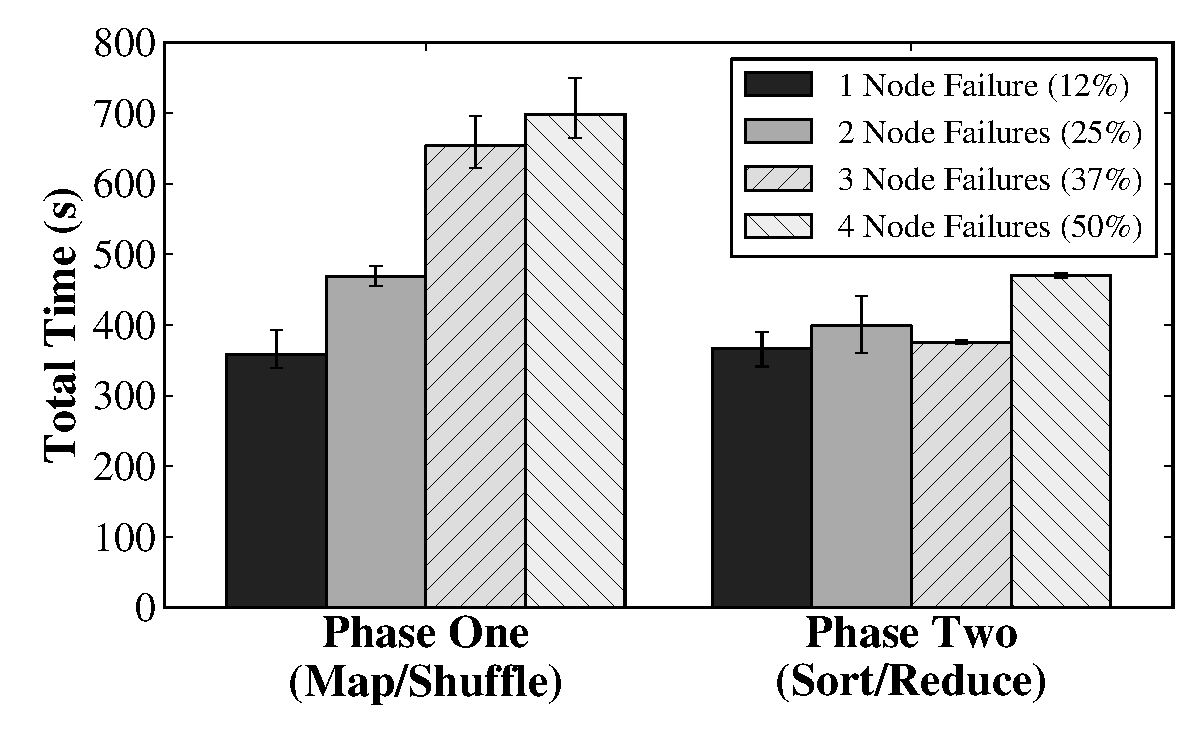
\includegraphics[width=\columnwidth]{fault_tolerance/graphs/node_recovery_proportionality.pdf}
  \caption{\label{fig:node_recovery_proportionality} Runtime of recovery from
    node failures during an 800GB sort.}
\end{figure}

To test the proportionality of recovery from node failure, we ran the same
800GB sort job as in the disk failure tests, but instead of failing individual
disks, we killed all \themis-related processes on a set of nodes approximately
120 seconds after starting the job. Each DFS disk's input consists of ten
evenly-sized files, each approximately 1.6GB
long. Figure~\ref{fig:node_recovery_proportionality} shows the elapsed time of
both phases of the recovery jobs for these failures.

Phase one's recovery time increases drastically as the number of failures
increase. The primary reason for this is that the same amount of recovery must
be done across an increasingly small number of nodes. Recovery time in phase
one is further increased by the fact that nodes are typically not accessing the
whole-file-replicated primary replica of the files they are recovering; as a
result, read performance degrades to that of unmodified HDFS.

Phase two's recovery time increases sub-linearly for the same architectural
reasons that it increases sub-linearly during disk recovery. Due to end-of-file
acknowledgments, only a small number of duplicate records are generated. As a
result, phase two's node recovery is roughly equivalent to scan-sharing phase
two of a normal 800GB sort with a disk recovery for all of the failed nodes'
disks.

\begin{figure}[t]
  \centering
  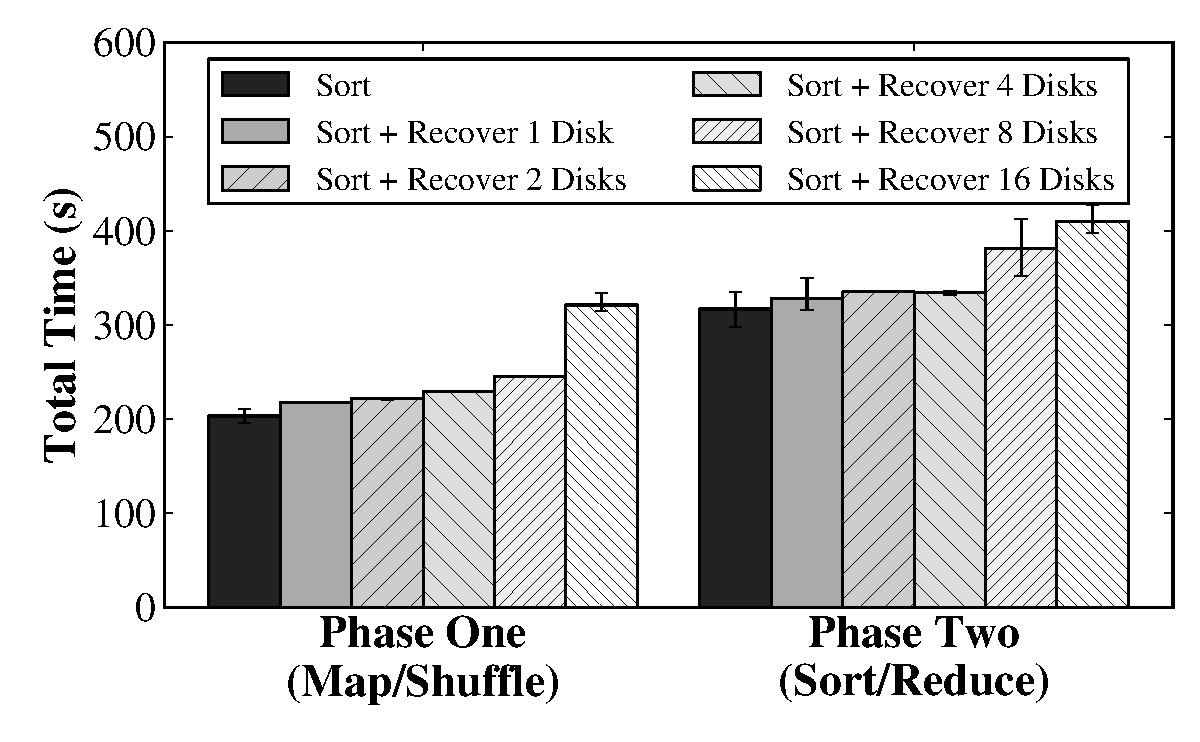
\includegraphics[width=\columnwidth]{fault_tolerance/graphs/scan_share_overhead.pdf}
  \caption{\label{fig:scan_sharing_overhead} Comparing the baseline performance
    of an 800GB sort with the performance of scan-sharing that sort with disk
    failure recovery jobs.}
\end{figure}

\subsection{Scan Sharing Overhead}
\label{sec:scan_sharing_overhead}

To evaluate the overhead imposed on a normal job by scan-sharing it with a
recovery job, we ran an 800GB sort job scan-shared with the recovery jobs
described in Section~\ref{sec:disk_proportionality}. In
Figure~\ref{fig:scan_sharing_overhead}, we see that phase one's runtime remains
fairly flat until we scan-share the sort job recovery of eight disks. At this
point, the system is writing so much intermediate data to the remaining disks
that it transitions from being bound by the speed at which it can read from
HDFS to being bound by the speed at which it can write to its intermediate
disks. At the same time, the amount of intermediate data produced by the
recovery job becomes large enough to visibly impact phase two.

\section{Conclusions}

MapReduce's traditional approach to fault tolerance is proportional, but it
imposes the overhead of additional rounds of I/O in common-case operation,
which negatively impacts the system's overall performance. In this work, we
have shown that, through leveraging the multi-tenancy typical of a MapReduce
cluster and composing previously-known fault tolerance techniques, it is
possible to provide proportional fault tolerance without imposing additional
rounds of I/O in failure-free operation.

\section{Acknowledgments}

This work was sponsored in part by NSF Grants CSR-1116079 and MRI CNS-0923523,
and through donations by Cisco Systems and a NetApp Faculty Fellowship.

Chapter~\ref{chapter:fault_tolerance} contains material as it appears in the
Proceedings of the ACM Symposium on Cloud Computing (SOCC) 2012. Rasmussen,
Alexander; Porter, George; Vahdat, Amin. The dissertation author was the
primary investigator and author of this paper.

Chapter~\ref{chapter:fault_tolerance} contains material submitted for
publication as ``I/O-Efficient Fault Tolerance for MapReduce''. Rasmussen,
Alexander; Porter, George; Vahdat, Amin. The dissertation author was the
primary investigator and author of this paper.



\chapter{Conclusions and Future Directions}
\label{chapter:conclusions}

Existing large-scale data processing systems scale out quite well, but do not
scale up; put another way, they do not utilize their clusters' resources to
nearly the extent that they should. In this dissertation, we have presented
two systems that illustrate the substantial gain in per-node efficiency that
can be realized if a minimal amount of efficiently-performed I/O is considered
as a first-class architectural concern.

In this chapter, we summarize the systems presented in this dissertation, and
discuss Themis's present limitations and some possible future research
directions.

\section{Summary}

With TritonSort, we have shown that a particular representative problem in this
space, large-scale sorting, can be performed at close to the maximum throughput
of the cluster through careful management of system resources to ensure
cross-resource balance. TritonSort's architecture is based on two central,
intuitive principles:

\begin{itemize}
  \item \textbf{When possible, write in large, sequential chunks.} The
    reasoning behind this principle applies mainly to magnetic hard drives, due
    to these devices' physical characteristics. TritonSort's user-level, global
    disk management subsystem performs fine-grained, dynamic buffering in front
    of a node's disks to ensure that writes are large and sequential even when
    the performance of a given disk is variable.
  \item \textbf{Read and write as little as possible.} Since secondary storage
    is likely to remain the bottleneck for large-scale data processing well
    into the future, it is critical that data processing systems read and write
    to secondary storage as little as possible. TritonSort's two phase external
    sort pipelines records aggressively; it reads and writes each record
    exactly twice, the theoretical lower bound for external sorting.
\end{itemize}

With Themis, we showed that TritonSort's two central principles could be
applied to a wider class of data-intensive problems. However, in order to
achieve similar performance benefits for general-purpose problems, we had to
significantly overhaul the way that we managed memory and partition
intermediate data adaptively. The resulting sampling and user-level memory
management systems allow for fine-grained, policy-driven control of memory
access in a way that allows jobs running in Themis to make progress in the face
of significant amounts of skew without creating stragglers. Themis executes a
wide range of MapReduce jobs with significantly higher per-node efficiency than
existing systems.

The aggressive pipelining adopted by both TritonSort and Themis comes at a
cost; the loss of any intermediate data requires that it be recomputed, since
it was only materialized in one place. We have shown that, in many scenarios,
the penalty imposed by complete re-computation on failure is significantly less
than the performance penalty of intermediate materialization. Further, we have
presented a modification to Themis that allows for proportional recovery from
faults. The central principle of this recovery mechanism is that by taking
advantage of the nature of multi-tenancy in modern MapReduce clusters and
relaxing the assumption that each intermediate record is created exactly once,
one can dramatically decrease the overhead of job re-execution.

We believe that this work holds a number of lessons for efficient
data-intensive system design and scale-out architectures in general, and will
help inform the construction of more efficient systems that will bridge the gap
between scalability and per-node efficiency.

\section{Limitations and Future Work}

Themis's high level of performance is predicated on its ability to tightly
control access to its host machine's I/O and memory. As a consequence, it is
unclear how Themis would perform when sharing a cluster of machines with other
applications. It is possible that some of Themis's features (such as its
unified control over disk I/O) might be incorporated into a lower-level service
that all processes could share, but we have not explored this approach.

At present, phase one of Themis's execution is limited by the speed of the
slowest node, and is thus negatively affected by stragglers. Since Themis does
not split its jobs into tasks, it is harder for it to support traditional
methods of straggler mitigation such as speculative execution. Investigating
alternate means of straggler mitigation is the subject of ongoing work.

A potential concern with the ``scan-and-discard'' method of fault tolerance
that we have not addressed in this work is the CPU overhead involved in
needlessly mapping input records whose intermediate data is not being
recovered. Modifying our approach to account for this overhead is the subject
of future work.

One clear avenue of future study is augmenting replicated storage systems like
HDFS so that they achieve performance close to that of raw disk. Our primary
whole-file replication approach, while fairly effective when the primary
replica is available, is admittedly fragile, and more adaptive or
workload-aware solutions could provide performance much closer to that of raw
disks.

Currently, the number of workers in each stage is fixed. To make the system
easier to configure, it would be valuable to dynamically determine the number
of workers that a stage needs to not bottleneck previous stages. A stage's
performance on synthetic data in isolation provides a reasonable upper-bound on
its performance, but any synthetic analysis does not take runtime conditions
such as CPU scheduling and cache contention into account. Therefore, some
manner of online learning algorithm will be necessary to determine a good
configuration at runtime.

Solid-state drives, or SSDs, are rapidly decreasing in cost per gigabyte but
have not approached the low price provided by magnetic hard
drives. Nevertheless, it is worth exploring the applicability of our design
principles to solid-state storage like SSDs and PCI-attached flash.

It is also worth exploring the applicability of our user-level memory
and disk management subsystems in a more general-purpose setting. For example,
languages like Pig and Hive that currently compile to a sequence of MapReduce
jobs could be compiled into a single distributed dataflow graph and thus forego
a great deal of often unnecessary intermediate data materialization.


% Stuff at the end of the dissertation goes in the back matter
\backmatter
\bibliographystyle{plain} % Or whatever style you want like plainnat
\bibliography{references}

\end{document}
